\part{Knowledge Discovery}
\label{partIV}

\chapter{Subspace Search in Data Streams}
\glsresetall
\label{chapter:subspacesearch}

This chapter builds on our contributions from Chapter \ref{chapter:MCDE} and \ref{chapter:S-MAB}. Our main results have not been officially published yet, but we present them in the following manuscript:
\begin{itemize}[noitemsep]
	\item \fullcite{DBLP:conf/review/FoucheKB20}
\end{itemize}
\textbf{Keywords:} Subspace Search; Data Stream Monitoring; Outlier Detection

\section{Chapter Overview}

In the real world, data streams are ubiquitous -- think of network traffic or sensor data. Mining patterns, e.g., outliers or clusters, from such data must take place in real time. This is challenging because (1) streams often have high dimensionality, and (2) the data characteristics may change over time. 
Existing approaches tend to focus on only one aspect, either high dimensionality or the specifics of streams. For static data, a common approach to deal with high dimensionality -- known as subspace search -- extracts low-dimensional, `interesting' projections (subspaces), in which patterns are easier to find.

However, searching for subspaces is difficult with static data already, because the number of subspaces increases exponentially with dimensionality. In \cite{DBLP:books/sp/Aggarwal2013}, Aggarwal compared the task of finding a pattern (e.g., an outlier) in high-dimensional spaces to that of searching for a needle in a haystack, while the haystack is one from an exponential number of haystacks. At the same time, \cite{DBLP:journals/ijdsa/TrittenbachB19} showed that to ensure high-quality results, the set of subspaces found must also be diverse, i.e., have low redundancy.

The streaming setting comes as an additional but orthogonal challenge. 
Stream mining algorithms are complex and must satisfy several constraints \cite{doi:10.1198/1061860032544} (see Section~\ref{challenges:datastreams}). While a periodic recomputation of existing, static methods may cope with \hyperlink{C2}{\textbf{C2}} (Single Scan) and \hyperlink{C3}{\textbf{C3}} (Adaptability), this is not efficient (\hyperlink{C1}{\textbf{C1}}) and results may not be available in an anytime fashion (\hyperlink{C4}{\textbf{C4}}). Last but not least, data streams may also be heterogeneous (\hyperlink{C5}{\textbf{C5}}). Considering these challenges, the analogy above becomes more complex: The haystacks (subspaces) of interest are not only hidden but also change over time.%, together with the location of the needle. 

In this chapter, we address those challenges by extending the idea of subspace search to data streams. We propose a new approach, \gls{SGMRD}, to monitor subspaces of interest in high-dimensional data streams. 
In a nutshell, we show that (1) our approach leads to efficient monitoring of relevant subspaces, and (2) such monitoring also improves subsequent Knowledge Discovery tasks, such as outlier detection. We compare our approach to competitive baselines and state-of-the-art methods. We release our source code and benchmark on GitHub\footnote{\url{https://github.com/edouardfouche/SGMRD}}, to ensure reproducibility. 

\section{Problem Formulation}

\subsection{Dimension-Based Subspace Search}

Subspace search in the static setting has already been formalised in the literature. The goal is to find a set of subspaces that fulfils a specific notion of optimality. Such subspaces must at the same time (1) be likely to reveal patterns (the `haystacks' from the analogy above) and (2) be diverse, i.e., have low redundancy with each other. 

To this end, the idea is to deem a set of subspaces optimal if adding or removing a subspace to/from this set makes the search results worse. 
To ensure diversity, the notion of optimality of each subspace must be tied to a specific dimension. This way, the resulting set may consist of the best subspaces w.r.t.\ each dimension, and each dimension is represented in this manner. This is the essence of what we call `dimension-based' search. 

To illustrate this, we show in Figure \ref{fig:GMD_example} an exemplary result from a dimension-based search and from another scheme. Dimension-based results are more diverse compared to other results, which tend to over-represent some dimensions. Previous work \cite{DBLP:journals/ijdsa/TrittenbachB19} showed that the diversity from dimension-based approaches is key to improve the performance of subspace search algorithms. 
\begin{figure}
	\centering
	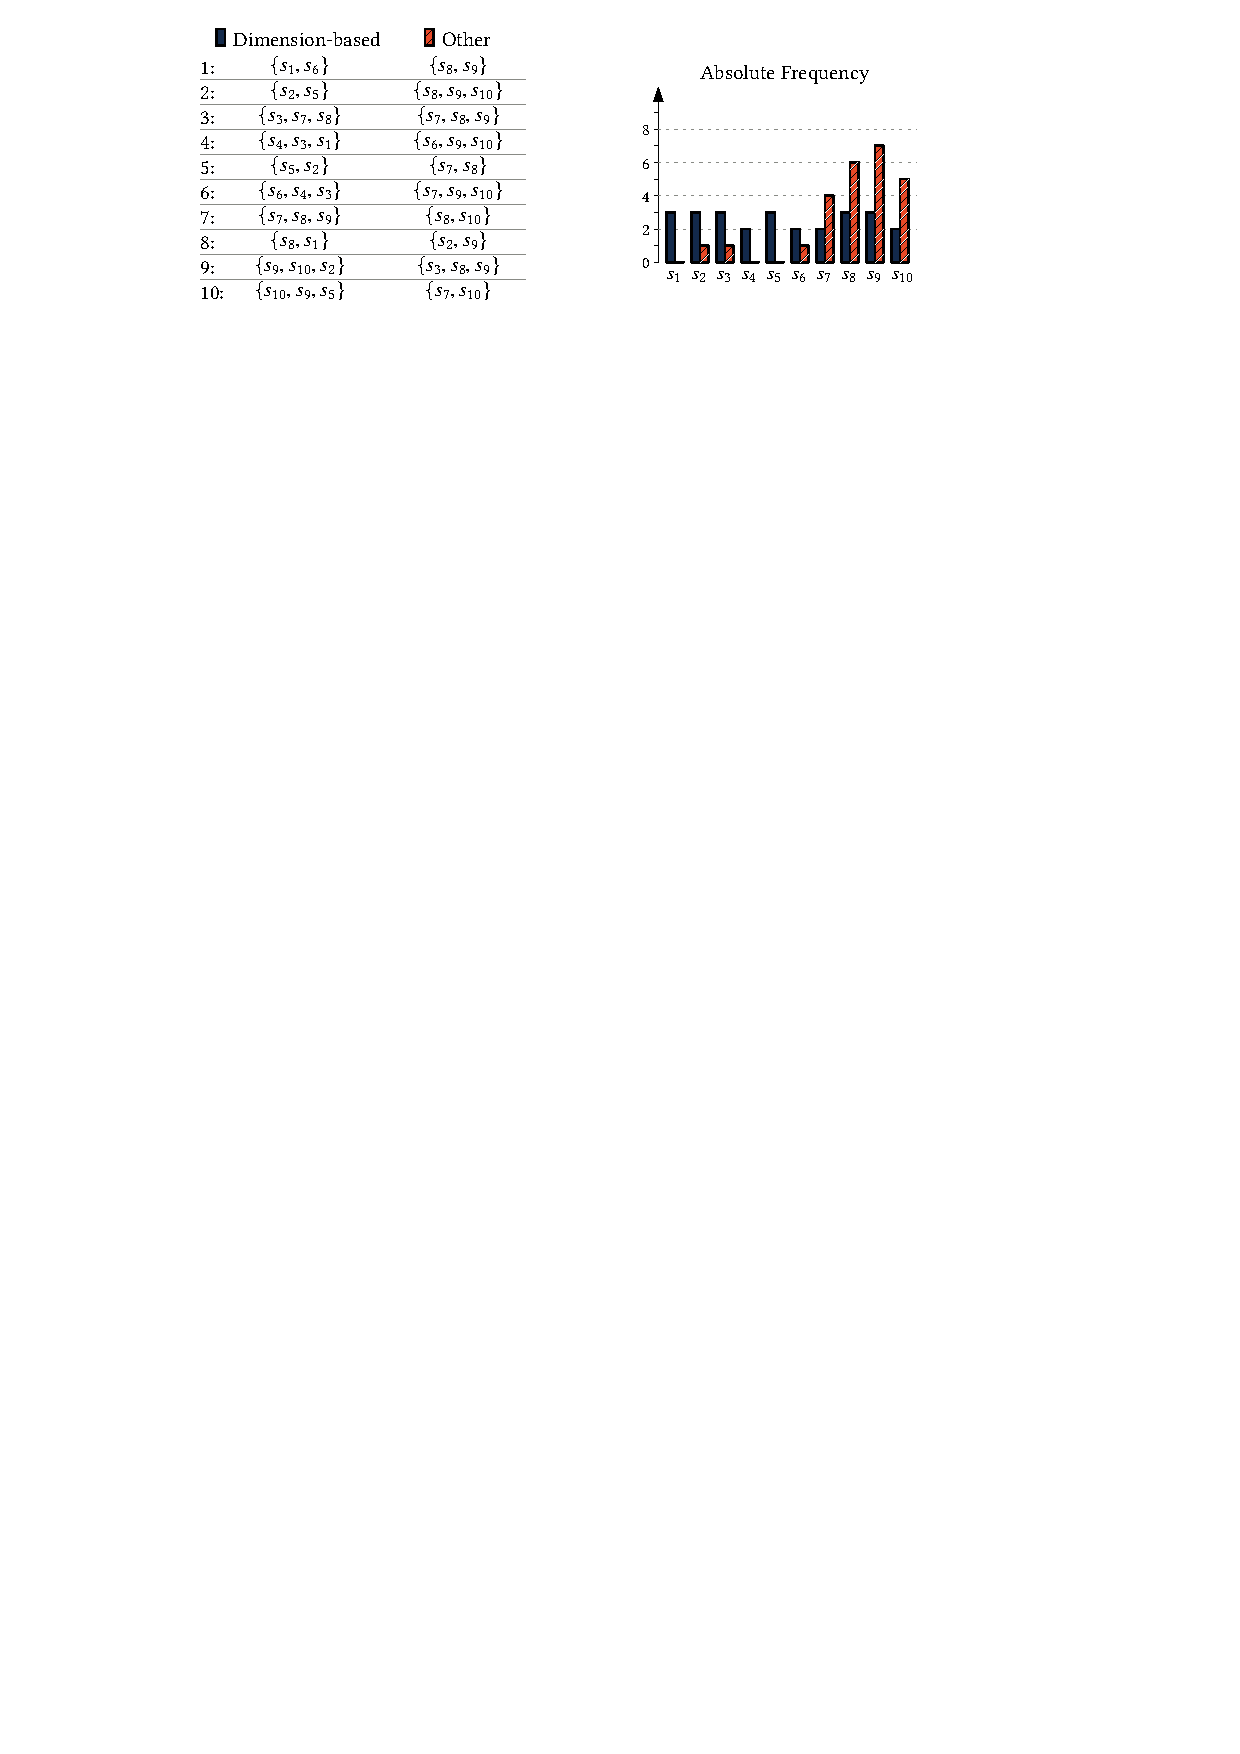
\includegraphics[width=0.9\linewidth]{part4-figures/example_gmd-compressed.pdf}
	\caption{Dimension-based subspace search versus other methods ($d=10$).} 
	\label{fig:GMD_example}
\end{figure} 

Formally, we define a so-called \gls{D-SQF}, to capture how much a dimension $s_i$ helps to reveal patterns in a subspace $S$:  
\begin{definition}[\gls{D-SQF}]
	\label{def:sqf}
	For any $ {\gls{S}} \in \gls{P}( \gls{D})$ and any $ \gls{s_i} \in  \gls{D}$, a \acrfull{D-SQF} is a function of type $\gls{q}:   \gls{P}( \gls{D}) \times  \gls{D}  \mapsto [0,1]$ with $\gls{q}(\gls{S}, \gls{s_i}) = 0, \forall  \gls{s_i} \notin  \gls{S}$.
\end{definition}
$\gls{q}(\gls{S}, \gls{s_i})=1$ means that $\gls{S}$ has the maximum potential to reveal patterns w.r.t.\ $\gls{s_i}$. Put differently, patterns may become more visible as one includes $\gls{s_i}$ in $\gls{S}$. 
In turn, $\gls{q}(\gls{S}, \gls{s_i})=0$ means that $\gls{S}$ cannot reveal any patterns w.r.t.\ $\gls{s_i}$. By definition, $\gls{q}(\gls{S}, \gls{s_i})=0$ if $\gls{s_i}$ is not part of $\gls{S}$ because the subspace cannot reveal any pattern in $\gls{s_i}$. 

Recent studies \cite{DBLP:conf/aaai/WangRNBMX17, DBLP:journals/ijdsa/TrittenbachB19} instantiate such \gls{D-SQF} as a measure of correlation, which one can estimate without any ex-post evaluation, i.e., it is not specific to any Data Mining algorithm. With this, subspace search remains independent of any downstream task. 
%\cite{DBLP:conf/icde/KellerMB12, DBLP:conf/sdm/BohmKMNV13, DBLP:conf/bigdataconf/NguyenMB13, DBLP:conf/sdm/NguyenMV16, DBLP:conf/aaai/WangRNBMX17, DBLP:journals/ijdsa/TrittenbachB19},
We can define a notion of subspace optimality: 
\begin{definition}[Optimal Subspace]
	A subspace $ \gls{S} \in   \gls{P}( \gls{D})$ is optimal w.r.t.\ $ \gls{s_i} \in  \gls{D}$ and a \gls{D-SQF} $\gls{q}$ if and only if 
	\begin{align*}
	\gls{q}( \gls{S},  \gls{s_i}) \geq  \gls{q}(S',  \gls{s_i}) \quad \forall S' \in  \gls{P}( \gls{D}).
	\end{align*}
\end{definition}
Then the optimal subspace set $\gls{SS*}$ is the set of optimal subspaces in $\gls{D}$ for all $\gls{s_i} \in \gls{D}$:
\begin{definition}[Optimal Subspace Set] \label{def:optimalset} A set $\gls{SS*}$ is optimal w.r.t.\ $\gls{D}$ and a Dimension-Subspace Quality Function (\gls{D-SQF}) $ \gls{q}$ if and only if
	\begin{align*}
	\forall \gls{s_i} \in \gls{D},~ \exists \gls{S} \in \gls{SS*} ~s.t.~ \forall S' \in \gls{P}(\gls{D}),~ \gls{q}(\gls{S},\gls{s_i}) \geq \gls{q}(S',\gls{s_i}).
	\end{align*}
\end{definition}
Thus, the optimal set $\gls{SS*}$ contains one subspace $\gls{S}$ for each dimension $ \gls{s_i} \in \gls{D}$, each one maximising the quality $ \gls{q}$ w.r.t.\ $ \gls{s_i}$. 
In other words, we can see $\gls{SS*}$ as a mapping of each dimension $ \gls{s_i} \in \gls{D}$ to an optimal subspace w.r.t.\ that dimension: 
\begin{align*}
\gls{SS*}:  \gls{s_i} \in  \gls{D} \mapsto  \gls{S} \in   \gls{P}(\gls{D}) \quad s.t. \quad \forall S' \in   \gls{P}(\gls{D}) \quad  \gls{q}(\gls{S}, \gls{s_i}) \geq  \gls{q}(S', \gls{s_i}).
\end{align*}

Finding $\gls{SS*}$ is NP-hard \cite{DBLP:phd/dnb/Nguyen15d}. 
This is because one needs to assess the \gls{D-SQF} of a set whose size grows exponentially with the number of dimensions. In fact, even finding a single optimal subspace is NP-hard. Thus, existing techniques do not guarantee the optimality of the results, but instead target at a good approximation of $\gls{SS*}$, while keeping the number of subspaces considered small. 

This idea is suitable in the static setting \cite{DBLP:conf/icde/KellerMB12, DBLP:conf/aaai/WangRNBMX17}. \cite{DBLP:journals/ijdsa/TrittenbachB19} showed that it leads to diverse sets of subspaces with better downstream mining results. 
Here, we propose a generalisation for streams. 

\subsection{Dimension-Based Subspace Search in Data Streams}
\label{sec:adaptation-stream}

The quality of subspaces, estimated via statistical correlation measures, may change over time, manifesting a phenomenon known as `concept drift' \cite{DBLP:conf/ictai/BarddalGE15} (see Section~\ref{challenges:datastreams}). Thus, in streams, the quality function $\gls{q}$ is time-dependent, and so we write  $\gls{SS*}$ and $\gls{qt}$. Then, the problem becomes more complex --- observe the following example:

\begin{example}[Variation of Mutual Information]
	\label{example:mutual_information}
	We obtained measurement data from the Bioliq power plant (cf. Section \ref{sec:bioliqexample}) and computed the evolution  of Mutual Information between a set of 10 sensor pairs for a single day. Figure \ref{fig:MI_evolution} graphs the results. The Mutual Information for pairs $1$ and $2$ remains stable for the whole duration, while it is more volatile for pairs $3$ to $6$. The pairs $7$ to $10$ in turn show some change, but with less variance. 
\end{example}

\begin{figure}
	\centering
	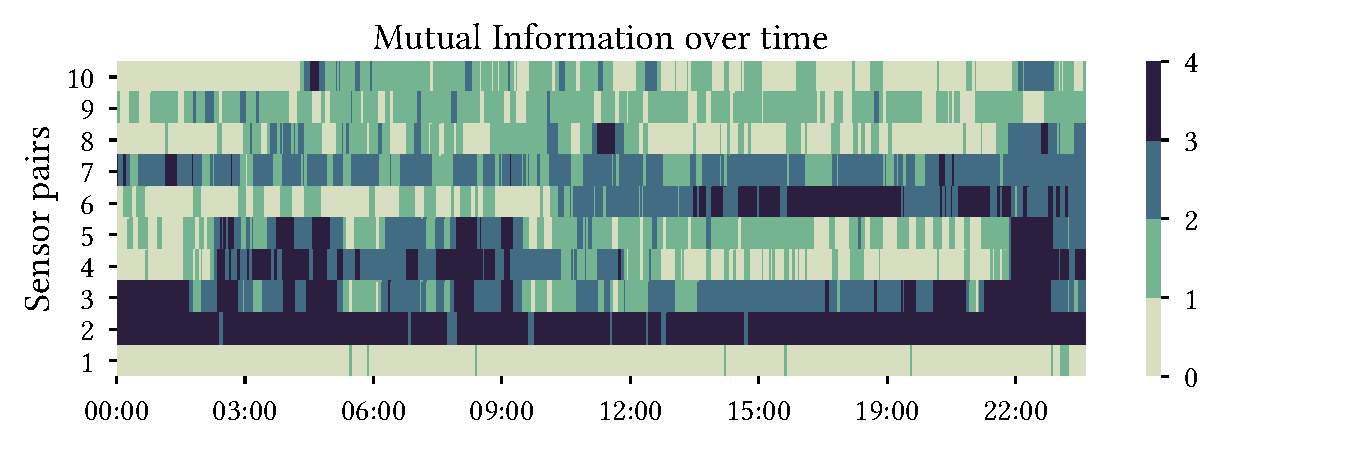
\includegraphics[width=0.9\linewidth, trim=0 0 2cm 0]{part4-figures/evolution_mutual_information_thesis-compressed.pdf}
	\caption{Evolution of Mutual Information between 10 sensor pairs at \acrshort{Bioliq}.} 
	\label{fig:MI_evolution}
\end{figure} 

As the example shows, some subspaces remain optimal for a longer period of time, while others frequently become sub-optimal. 
So the difficulty is that, even if one finds the set of subspaces $\gls{SS*t}$, there is no guarantee that this set is optimal at time $\gls{t}+1$. Next, it is impossible to even test the optimality of $\gls{SS*}$, because one would need to evaluate an exponential number of subspaces.

Let us assume that the cost of evaluating the quality of a subspace is constant across different subspaces and time. This is the case when considering existing correlation estimators. We define a function $\mathcal{E}_t: \gls{P}(\gls{D}) \times \gls{D} \mapsto \{0,1\}$ such that $\mathcal{E}_t(\gls{S}, \gls{s_i}) = 1$ if one computes $\gls{qt}(\gls{S},\gls{s_i})$, otherwise $0$. We can now formulate subspace search in data streams as a multi-objective optimisation problem at time $\gls{t}$ with two conflicting objectives: %EF: See for example https://en.wikipedia.org/wiki/Multi-objective_optimization
\begin{enumerate}[noitemsep] 
	\item Find a set $\gls{SSt}$ which approximates $\gls{SS*t}$ well. 
	I.e., minimise the sum of the differences between the quality of the optimal set and the quality of the approximate set for each dimension. This is the first objective $O_1 = \sum_{i=1}^{|\gls{D}|} \left[\gls{qt}(\gls{SS*t}(\gls{s_i}),\gls{s_i}) - \gls{qt}(\gls{SSt}(\gls{s_i}),\gls{s_i})\right]$.
	\item Reduce the computation of the search, i.e., minimise the number of subspaces for which one computes the quality at time $\gls{t}$. This is objective $O_2 = \sum_{\gls{s_i}}^{\gls{D}} \sum_{\gls{S}}^{ \gls{P}(\gls{D})} \mathcal{E}_{t}(\gls{S}, \gls{s_i})$.
\end{enumerate}
If $O_1 = 0$, then $\gls{SSt} \equiv \gls{SS*t}$. Conversely, if $O_2 = 0$, then choosing $\gls{SSt}$ boils down to random guessing. Thus, objectives $O_1$ and $O_2$ conflict. They capture the trade-off between the quality of the set of subspaces and the computation effort. 

Definition \ref{def:optimalset} implies that the search is independent for each dimension. Thus, to optimise $O_1$, we must find a dimension-based search algorithm, which for any dimension $\gls{s_i} \in \gls{D}$, returns a near-optimal subspace $\gls{S}$ w.r.t.\ the dimension. More formally: 

\begin{definition}[Dimension-based Search Algorithm]
	We define a dimension-based search algorithm as a function $\textsc{Search}_t: \gls{D} \mapsto \gls{P}(\gls{D})$, which for any dimension $\gls{s_i} \in \gls{D}$, returns a subspace $\gls{S}$ minimising  $\gls{qt}(\gls{SS*t}(\gls{s_i}),\gls{s_i}) - \gls{qt}(\gls{S},\gls{s_i})$ at time $\gls{t}$. 
\end{definition}

Such an algorithm is associated with a cost, which depends on the number of subspaces evaluated. I.e., each run of $\textsc{Search}_t$ negatively impacts objective $O_2$. Thus, an additional challenge is to find an update policy $\pi: \gls{t} \mapsto \gls{P}(\gls{D})$ to decide at any time, for which dimension(s) one should repeat the search. We define it as follows: 

\begin{definition}[Update Policy]
	An update policy is a function $\pi: \gls{t} \mapsto \gls{P}(\gls{D})$ which returns $\forall \gls{t}$ a set $\gls{I(t)} \in \gls{P}(\gls{D})$, so that one repeats the $\textsc{Search}_t$ algorithm for $\gls{s_i} \in \gls{I(t)}$.    
\end{definition}

Overall, to achieve subspace search in data streams, we must come up with an adequate instantiation of the following elements:  

\begin{itemize}[noitemsep] 
	\item A quality measure $\gls{qt}: \gls{P}(\gls{D}) \times \gls{D}  \mapsto [0,1]$.
	\item A dimension-based search algorithm $\textsc{Search}_t: \gls{D} \mapsto \gls{P}(\gls{D})$. 
	\item An update policy $\pi: \gls{t} \mapsto \gls{P}(\gls{D})$.
\end{itemize}

Our approach, \acrfull{SGMRD}, addresses the challenges described previously by instantiating and combining each of these elements in a general framework. % in an effective way. In what follows, we describe the specifics of SGMRD. 

\section{Subspace Search in Data Streams}

\subsection{Our Approach: \acrshort{SGMRD}}

Figure~\ref{fig:SGMRD_workflow} shows an overview of our framework, which consists of two steps: 
\begin{enumerate}[noitemsep]
	\item \textbf{Initialisation}. We find an initial set of subspaces $\mathbb{S}_0$, using the first $\gls{w}$ observations in the stream. 
	To do so, we run the algorithm $\textsc{Search}_t$ for each dimension. 
	The outcome of this step is a set of subspaces $\gls{S}_1, \dots, \gls{S}_d$, one for each dimension. 
	\item \textbf{Maintenance}. For any new observation in the stream, we monitor the quality of subspaces $\gls{qt}(\gls{S}, \gls{s_i})$ for $\gls{S} \in \gls{SSt}$, and decide, by learning a policy $\pi$, for which dimension(s) we repeat the search, i.e., algorithm $\textsc{Search}_t$. 
\end{enumerate}

Our approach is general to some extent, as one could consider various instantiations of each building block (Search, Monitor and Update). With SGMRD, we instantiate the search function $\textsc{Search}_t$ as a greedy hill-climbing heuristic,  $\gls{qt}$ as an efficient dependency estimator, MCDE (Chapter \ref{chapter:MCDE}), and the policy $\pi$ as a Multi-Armed Bandit (MAB) algorithm with variable number of plays, S-MAB (Chapter \ref{chapter:S-MAB}). We describe the specifics of each block and explain our design decisions in the following sections. 

\begin{figure*}
	\centering
	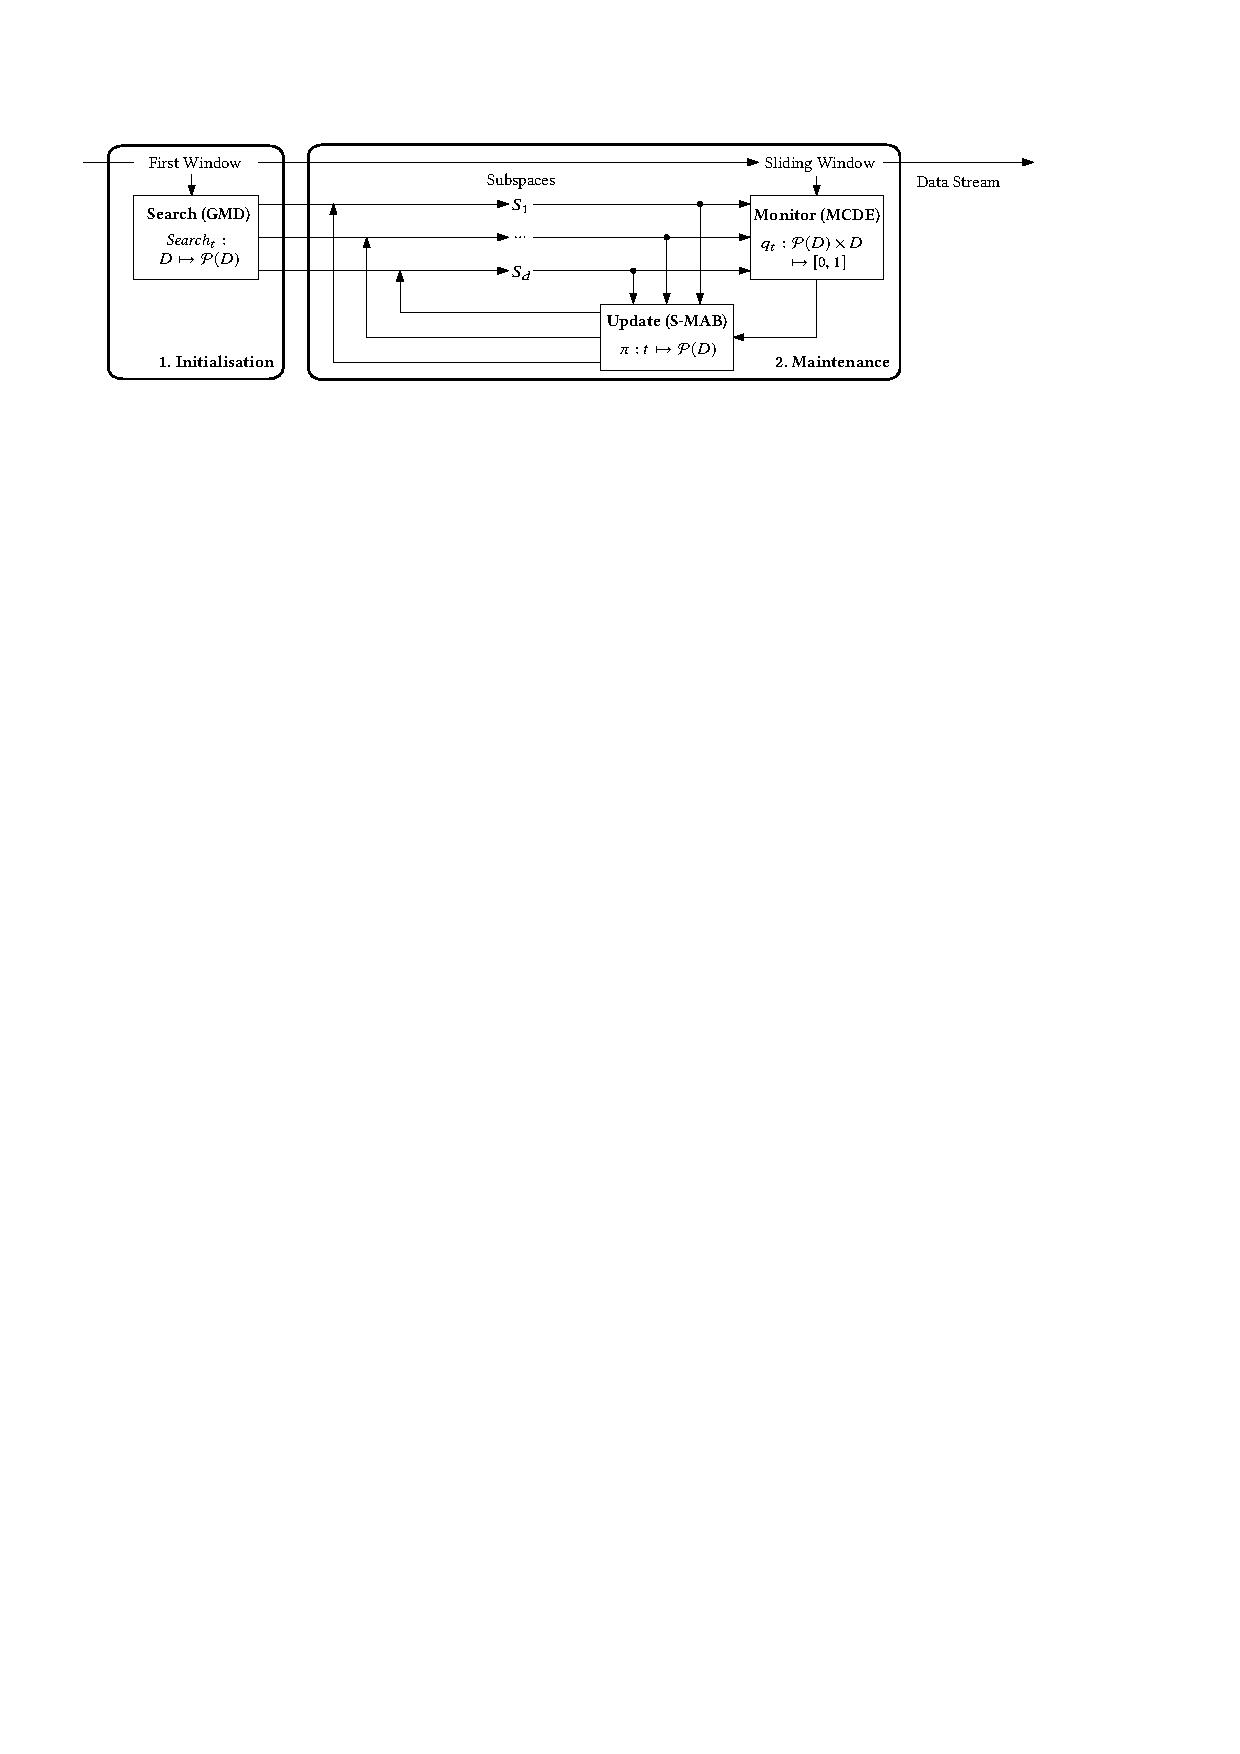
\includegraphics[width=\linewidth]{part4-figures/SGMRD_workflow_small_2-compressed.pdf}
	\caption{\acrshort{SGMRD}: A High-Level Overview.} 
	\label{fig:SGMRD_workflow}
\end{figure*} 

\subsubsection{Search}

{SGMRD}'s initialisation searches for an initial set of subspaces using the first observation window. Since finding the optimal set (cf.\ Definition~\ref{def:optimalset}) is not feasible, we instantiate $\textsc{Search}_t$ as a greedy hill-climbing heuristic. Our heuristic constructs subspaces in a bottom-up manner. 
Algorithm~\ref{alg:greedysearch} is our pseudo-code, and Figure \ref{fig:SGMRD_gmd} illustrates our idea.% with a toy example.% with only four dimensions.  

\begin{figure}
	\centering
	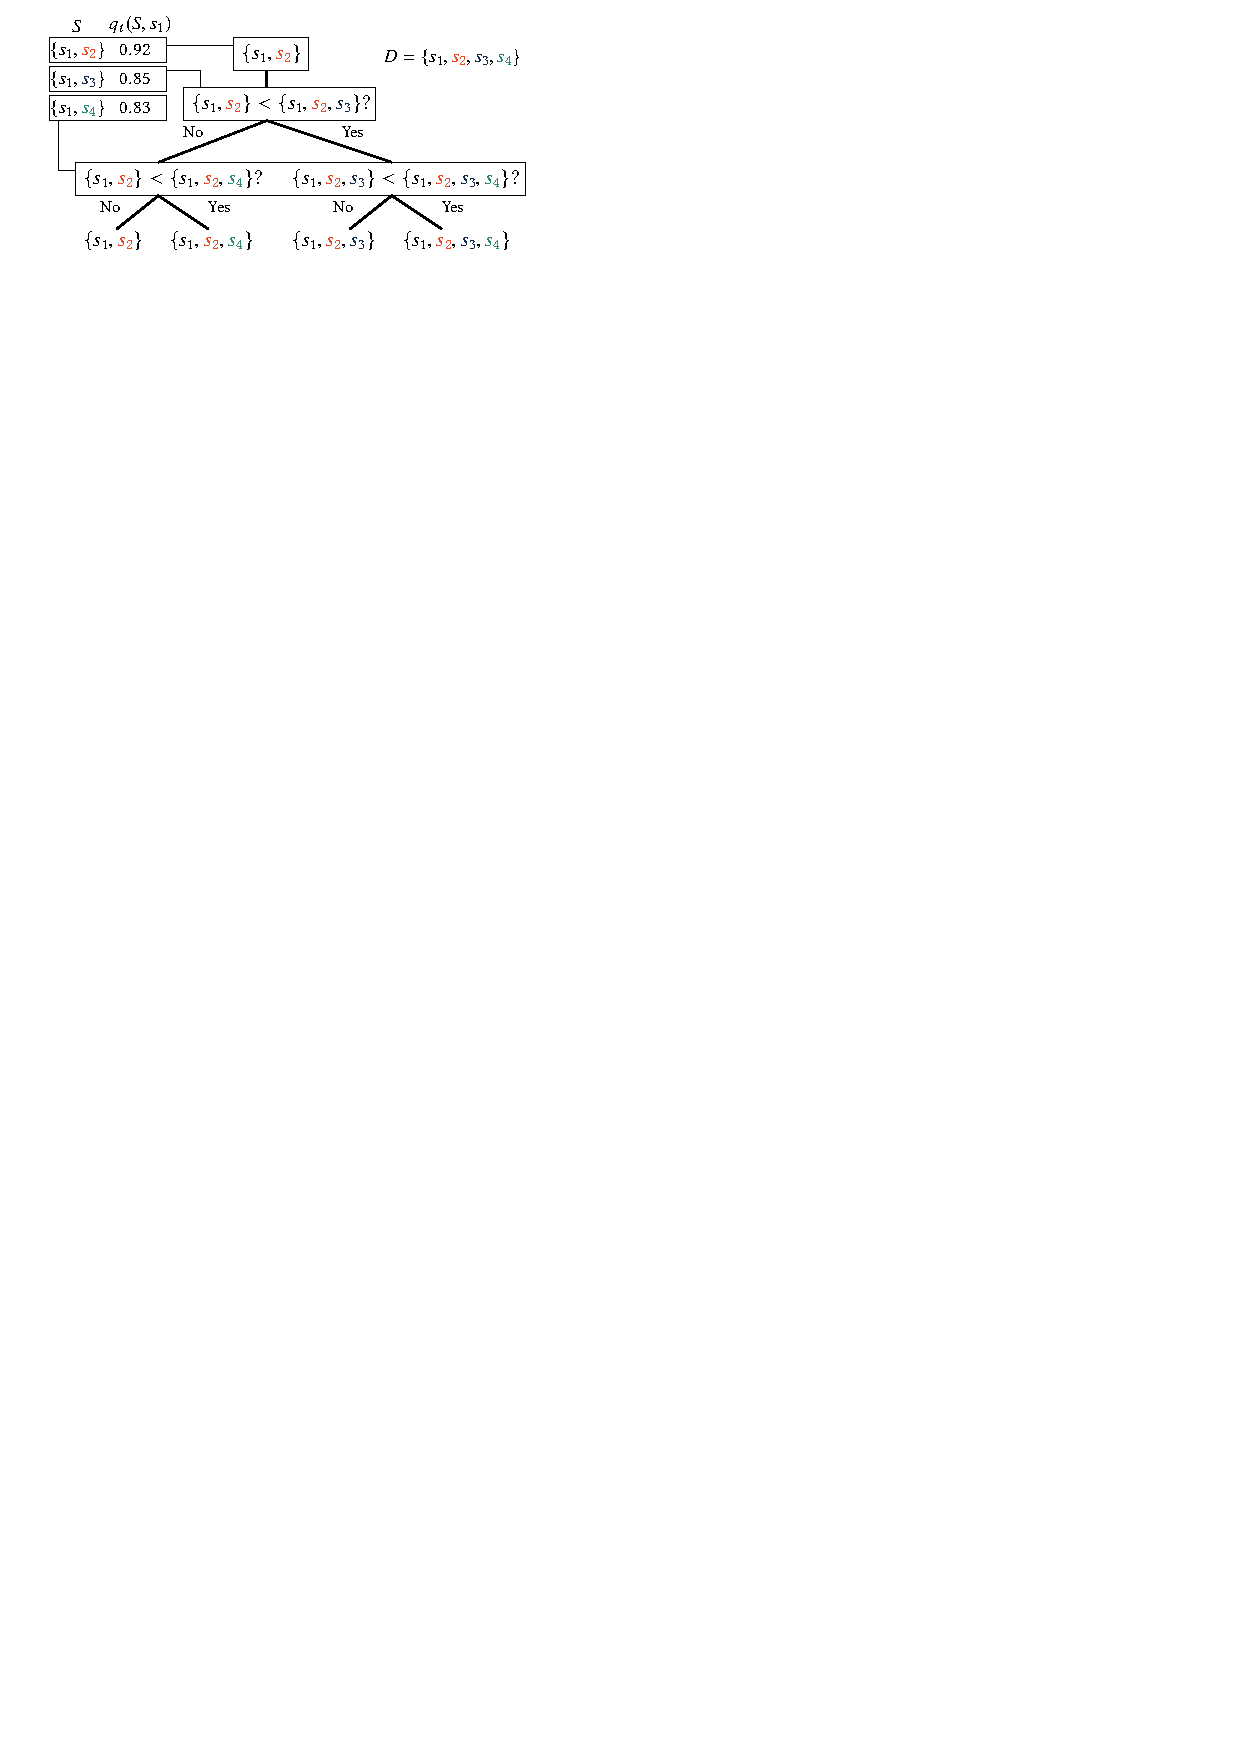
\includegraphics[width=0.7\linewidth]{part4-figures/SGMRD_gmd-compressed.pdf}
	\caption{Example of search w.r.t.\ $s_1$ with four dimensions.} 
	\label{fig:SGMRD_gmd}
\end{figure} 

In a first step (Line \ref{alg:greedysearch:line1}), we select the 2-dimensional subspace maximising the quality w.r.t.\ $\gls{s_i}$. In our example, $\gls{s_i} = s_1$, and the subspace with the highest quality is $\{s_1, s_2\}$. Then, we iteratively test whether adding the dimension associated with the next best 2-dimensional subspace containing $\gls{s_i}$ (Line \ref{alg:greedysearch:line4}) increases the quality of the current subspace (Line \ref{alg:greedysearch:line5}). If this is the case, we add it into the current subspace (Line \ref{alg:greedysearch:line6}), otherwise, we discard it. In our example, the heuristic first considers adding $s_3$, then $s_4$. 

The advantage of only considering 2-dimensional subspaces is that it keeps the runtime of the search linear w.r.t.\ the number of dimensions. More precisely, we can see that the heuristic computes the quality of exactly $(|\gls{D}|-1) + (|\gls{D}|-2) = 2|\gls{D}| -3$ subspaces. Thus, the runtime of Algorithm \ref{alg:greedysearch} is in $O(|\gls{D}|)$. The search is independent for each dimension. At initialisation, we run it for each dimension, so the initialisation is in $O(|\gls{D}|^2)$.

\begin{algorithm}
	\footnotesize
	\caption{$\textsc{Search}_t$($\gls{s_i}$)}\label{alg:greedysearch} 
	\begin{algorithmic}[1]
		\Require A dimension/attribute $\gls{s_i} \in \gls{D}$ 		
		\State $\gls{SSS}^{\mathit{max}} \gets \gls{s_i} \cup \left (\argmax_{s_j \in \gls{S}} \gls{qt}(\gls{s_i} \cup s_j, \gls{s_i}) \right ) $ \label{alg:greedysearch:line1}
		\State $\gls{S} \gets \gls{S} \setminus \gls{SSS}^{\mathit{max}}$
		\While{ $\gls{S}$ is not empty}
		\State $\gls{SSS}^{\mathit{cand}} \gets \argmax_{s_j \in \gls{S}} \gls{qt}(\gls{s_i} \cup s_j, \gls{s_i}) $ \label{alg:greedysearch:line4}
		\If{$\gls{qt}(\gls{SSS}^{\mathit{max}} \cup \gls{SSS}^{\mathit{cand}}, \gls{s_i}) > \gls{qt}( \gls{SSS}^{\mathit{max}}, \gls{s_i})$} \label{alg:greedysearch:line5}
		\State $\gls{SSS}^{\mathit{max}} \gets \gls{SSS}^{\mathit{max}} \cup \gls{SSS}^{\mathit{cand}}$ \label{alg:greedysearch:line6}
		\EndIf
		\State $\gls{S} \gets \gls{S} \setminus \gls{SSS}^{\mathit{cand}}$
		\EndWhile
		\State \textbf{return} subspace $\gls{SSS}^{\mathit{max}} \subseteq \gls{D}$
	\end{algorithmic}
\end{algorithm}

\subsubsection{Monitor}

So far, we did not discuss any concrete instantiation of the quality $\gls{qt}$. In practice, one has only a sample of observations, and thus, the quality can only be \textit{estimated} from a limited number of points. In what follows, we describe a new method to estimate the quality. Considering the constraints from the streaming setting and the nature of the required quality function, our method must fulfil the following technical requirements:

\textbf{Efficiency.} Since the search includes estimating the quality of numerous subspaces, the quality-estimation procedure must be efficient, to cope with the streaming constraints.  

\textbf{Multivariate.} Since subspaces can have an arbitrary number of dimensions, the quality measure must be multivariate. Traditional dependency estimators are bivariate  \cite{10.2307/2289859}.

\textbf{Asymmetric.} Since the quality values are specific to each dimension, the measure is not symmetric. The quality of subspace $\{s_1, s_2\}$ does not need to be the same w.r.t.\ $s_1$ or $s_2$.

We define the quality as a measure of non-independence in subspace $S$ w.r.t.\ $s_i$. Recall that Definition \ref{IA1} implies that the marginal distributions of each variable $\gls{X}_i \in \gls{X}$ must be equal to their conditional distribution w.r.t.\ $\gls{X} \setminus \gls{X}_i$. We can estimate the quality as a degree of non-independence w.r.t.\ a dimension $\gls{X}_i$, and quantify it as the discrepancy between the empirical marginal distribution $\hat{p}_{X_i}$ and the conditional distribution  $\hat{p}_{X_i|(X \setminus X_i)}$. For the ease of discussion, let us consider $\gls{qt}(\{s_1, s_2\}, s_1)$. Then,
\begin{align}
\gls{qt}(\{s_1, s_2\},s_1) \propto disc\left(\hat{p}_{s_1}, \hat{p}_{s_1|s_2}\right),
\end{align}
where $disc$ is the discrepancy between both distributions. 

To estimate this discrepancy, we propose a bootstrap method. Iteratively, we take a random condition w.r.t.\ the dimensions $S \setminus s_1$ (i.e., restricting the other dimensions to a random interval) and perform a statistical test between the sets of observations within and outside of this random condition w.r.t.\ $s_1$. This is the idea behind our main contribution from Chapter \ref{chapter:MCDE}, \gls{MCDE}. 

In the end, the quality is as follows:  
\begin{align}
\gls{q}(\gls{S}, \gls{s_i}) =
\sum_{m=1}^{M} \left [ \mathcal{T} \left(B\left(c_{i}  \right), B\left(\overline{c}_i\right)\right)\right ]
\end{align}
where $c_i$ is chosen randomly over $M$ independent iterations, but the condition $c_i$ is chosen such that $\gls{s_i}$ is the reference dimension (see also Equation \ref{def:contrast-approx}). The underlying statistical test $\mathcal{T}$ depends on the type of attribute $\gls{s_i}$. For example, if the attribute is of numerical type, we use the two-sample Kolmogorov-Smirnov test (see Section \ref{sec:instantiationMCDE}). 

Thus, our quality function inherits the benefits of \gls{MCDE}. The incremental index structure gives way to an efficient (\hyperlink{C1}{\textbf{C1}}) estimation of subspace quality on streams (see Section~\ref{adaptation-stream}). Our index operates on a sliding window, so it only requires a single scan (\hyperlink{C2}{\textbf{C2}}) and supports efficient insert/deletion operations. Furthermore, the anytime flexibility of \gls{MCDE} helps to control the trade-off between the accuracy of the search and execution time (\hyperlink{C4}{\textbf{C4}}). Finally, \gls{MCDE} handles heterogeneous streams (\hyperlink{C5}{\textbf{C5}}). 

To monitor the quality estimates of each subspace in $\mathbb{S}_t$ over time, we smooth out the statistical fluctuations of the estimation process via exponential smoothing with parameter $\gamma$ (as in Equation \ref{eq:exp-decay}). Previous experiments from Chapter \ref{chapter:MCDE} showed that $M=100$ with $\gamma = 0.9$ leads to good estimation quality and performance w.r.t.\ downstream tasks. The outcome is a smoothed quality function $Q_t: \gls{D}\mapsto [0,1]$:
\begin{align}
\label{eg:monitoring}
Q_{t+1}(\gls{s_i}) = \gamma \cdot \gls{qt}(\gls{SSt}(\gls{s_i}), \gls{s_i}) + (1- \gamma) \cdot \gls{q}_{\gls{t}+1}(\gls{SSt}(\gls{s_i}), \gls{s_i}).
\end{align}

\subsubsection{Update}
\label{sec:update}

The initialisation is expensive, because one needs to run the search (Algorithm \ref{alg:greedysearch}) for each dimension. While running the search for every dimensions optimises the quality of the subspace set (Objective $O_1$), it curbs efficiency (Objective $O_2$). However, as in Example \ref{example:mutual_information}, the dependence between dimensions can unexpectedly change over time. Thus, without any assumption, it is not possible to exploit our knowledge from step $\gls{t}-1$. We mitigate the computational cost over time by only repeating the search for a few dimensions. 

The challenge is to find a policy $\pi: \gls{t} \mapsto \gls{P}(\gls{D})$ to decide at any time step $\gls{t}$ for which $\gls{L}$ dimensions to repeat the search, where $\gls{L} < |\gls{D}|$ is a budget per time step. The budget $\gls{L}$ can either be set by the user, or it is based on the available computational time available between two subsequent observations. Basically, it is a trade-off between $O_1$ and $O_2$.

To solve this challenge, we cast the decisions of the policy $\pi$ as a MAB problem with multiple plays  \cite{DBLP:conf/alt/UchiyaNK10}. Multi-Armed Bandit (MAB) models are useful tools to capture the trade-offs of sequential decision making problems. 
We model each dimension $\gls{s_i} \in \gls{D}$ as an `arm'. 
In each round $\gls{t}=\{1,\dots,\gls{T}\}$, the policy $\pi$ selects $\gls{L} < |\gls{D}|$ arms $\gls{I(t)} \subset \gls{D}$ and runs the search for each $\gls{s_i} \in \gls{I(t)}$. Then, there are two possible outcomes for each $\gls{s_i}$:  
\begin{enumerate}[noitemsep]
	\item \textbf{Success}: $\textsc{Search}_t(\gls{s_i})$ yields a better subspace than $\mathbb{S}_{t-1}(\gls{s_i})$, 
	so we update $\gls{SSt}(\gls{s_i})$. The policy receives a reward of $1$. 
	\item \textbf{Failure}: $\textsc{Search}_t(\gls{s_i})$ does not yield a better subspace, so we set $\gls{SSt}(\gls{s_i}) \gets \mathbb{S}_{{{t}}-1}(\gls{s_i})$. The reward is $0$. 
\end{enumerate}

The \acrshort{S-MAB} model \cite{DBLP:conf/kdd/FoucheKB19} (Chapter~\ref{chapter:S-MAB}) provides an adequate framework to optimise the gains from the policy $\pi$ in such setting. Let each dimension be an arm, i.e., $\gls{K} = |\gls{D}|$. We associate arm $i \in [\gls{K}]$ with a Bernoulli distribution $\mathcal{B}_i$ with mean $\gls{mu_i}$. At each round $\gls{t} = 1, \dots, \gls{T}$, a policy selects a set of $\gls{L}_{\gls{t}}$ arms $\gls{I(t)} \subset [\gls{K}]$ and repeat the search for these arms/dimensions. The policy receives a reward vector $\gls{X(t)}$. The reward $\gls{X_i(t)} = 1$ if the search is successful, $0$ otherwise. Selecting an arm $i \in [\gls{K}]$ leads to a cost in $O(|\gls{D}|)$, normalised to $1$. The policy aims to maximise the sum of the rewards, but such that it is greater than the sum of the costs by an efficiency factor $\gls{eta^*} \in [0,1]$. The parameter $\gls{eta^*}$ models the trade-off between objective $O_1$ and $O_2$. If $\gls{eta^*} \approx 0$, then minimising $O_1$ (improving quality) is much more important than $O_2$ (reducing computation). Conversely, whenever $\gls{eta^*} \approx 1$, one must minimise computation as much as possible (see Section \ref{sec:STS}). 

Thus, we use \gls{S-TS} as an update strategy for \gls{SGMRD}. Algorithm~\ref{SGMRD-Update} is the pseudo-code for our strategy. We initialise the statistics for each arm/dimension, $\alpha_i$, $\beta_i$, $N_i$ and $S_i$ to $1$ and the initial number of plays $\gls{L} = |\gls{D}|$. The scaling policy, \gls{KL-S}, requires an additional parameter $\gls{eta^*}$, as discussed earlier (cf. Algorithm~\ref{S-TS}). 


\begin{algorithm}[ht]
	\footnotesize
	\caption{\textsc{Update}($\gls{SSt}$)}\label{SGMRD-Update} 
	\begin{algorithmic}[1]
		\Require A set of subspaces $\gls{SSt}$, A target efficiency $ \gls{eta^*}$ and number of plays $\gls{L}$ (For \textsc{\gls{KL-S}}, the scaling procedure)
		\For{$i = 1,\dots, \gls{K}$}  
		\State $\theta_i(t) \sim \text{Beta}(\alpha_i(t), \beta_i(t))$ 
		\EndFor 
		\State $ \gls{I(t)} := \argmax_{K' \subset [ \gls{K}], |K'| = \gls{L}} \sum_{i}^{K'}\theta_i(t)$
		\For{$i \in  \gls{I(t)}$}
		\State $S \gets \textsc{Search}_t(\gls{s_i})$  \Comment{Serarching for a new subspace w.r.t $\gls{s_i}$ (Algorithm \ref{alg:greedysearch})}
		\If{$\gls{q}_{\gls{t}+1}(\gls{S}, \gls{s_i}) > Q_{\gls{t}+1}(\gls{SSt}(\gls{s_i}), \gls{s_i})$ and $\gls{S} \neq \gls{SSt}(\gls{s_i})$} 
		\State $\mathbb{S}_{{\gls{t}}+1}(\gls{s_i}) \gets \gls{S}$
		\State $\gls{X_i(t)} \gets 1$
		\Else 
		\State $\mathbb{S}_{{\gls{t}}+1}(\gls{s_i}) \gets \gls{SSt}(\gls{s_i})$
		\State $\gls{X_i(t)} \gets 0$
		\EndIf
		\State $\alpha_i(t+1) = \alpha_i(t) +  \gls{X_i(t)}$  \Comment{Update parameters}
		\State $\beta_i(t+1) = \beta_i(t) + (1- \gls{X_i(t)})$ 
		\State $\gls{L} \gets \textsc{\gls{KL-S}}(\gls{L})$ \Comment{Scaling policy (Algorithm~\ref{S-TS})}
		\EndFor
		\State \textbf{return} $\mathbb{S}_{{\gls{t}}+1}$
	\end{algorithmic}
	
\end{algorithm}

\subsubsection{\gls{SGMRD}}

Algorithm \ref{alg:sgmrd} summarises our approach as pseudo-code. \gls{SGMRD} finds an initial set of subspaces using the first window (Line \ref{line:initialsearch}). 
Then SGMRD monitors and updates the set of subspaces (Line \ref{line:monitor} to \ref{line:update}) for each new observation $\vec{\gls{x}}_{{\gls{t}}+1}$. The parameter $v$ controls the frequency of the update steps. 

\begin{algorithm}
		\footnotesize
	\caption{\textsc{\gls{SGMRD}}($(\gls{D}$, $\gls{B}$), $\gls{w}$, $v, \gamma$)}\label{alg:sgmrd} 
	\begin{algorithmic}[1]
		\Require A data stream ($\gls{D},\gls{B}$), a window size $\mathit{\gls{w}} > 0$, the frequency of updates $v > 0$, decay $\gamma \in (0,1)$
		
		\State $\gls{t} \gets \gls{w}$ \Comment{\textbf{1. Initialisation}}
		\State $\gls{SSt} \gets \{\gls{s_i} : \textsc{Search}_t(\gls{s_i}), \forall \gls{s_i} \in \gls{D}\}$ \label{line:initialsearch} \Comment{Initial search. Algorithm \ref{alg:greedysearch}} 
		\While{$\gls{B}$ has a new observation $\vec{\gls{x}}_{{\gls{t}}+1}$}   \Comment{\textbf{2. Maintenance}}
		\State $\gls{t} \gets \gls{t} + 1$
		\For{$\gls{s_i} \in \gls{D}$} \label{line:monitor} \Comment{Monitoring}
		\State $Q_{t}({s_i}) = \gamma \cdot q_{t-1}(\mathbb{S}_{t-1}(\gls{s_i}), \gls{s_i}) + (1- \gamma) \cdot {q}_{{t}}(\mathbb{S}_t(\gls{s_i}), \gls{s_i})$  
		\EndFor
		\State \textbf{if} $\gls{t} - \gls{w} \equiv 0 \pmod{v}$ \textbf{then} $\gls{SSt} \gets \textsc{Update}(\mathbb{S}_{{\gls{t}}-1})$ \textbf{else} $\gls{SSt} \gets \mathbb{S}_{{\gls{t}}-1}$ \label{line:update} \Comment{Updating. Algorithm \ref{SGMRD-Update}}
		\EndWhile	
		\State \textbf{return at anytime} the set of subspaces $\gls{SSt}$ 
	\end{algorithmic}
\end{algorithm}

Overall, our method is efficient (\hyperlink{C1}{\textbf{C1}}), as our quality estimates can be computed in linear time. %, with adaptive accuracy by letting the number of iterations $M$ vary. 
It also requires a single scan of the data (\hyperlink{C2}{\textbf{C2}}), as we monitor subspaces over a sliding window. By design, \gls{SGMRD} adapts (\hyperlink{C3}{\textbf{C3}}) to the environment by updating the subspace search results with parsimonious resource consumption, and our experiments will confirm this. Finally, results are available at any point in time (\hyperlink{C4}{\textbf{C4}}). 

\subsection{Downstream Knowledge Discovery}
\label{sec:downstream}

High-quality subspaces can be useful for virtually any downstream Data Mining task. For example, previous work \cite{DBLP:conf/icde/KellerMB12,  DBLP:conf/sdm/NguyenMV16, DBLP:conf/aaai/WangRNBMX17, DBLP:journals/ijdsa/TrittenbachB19} leverages subspaces to build ensemble-like outlier detectors. Other Data Mining tasks are possible as well, such as clustering \cite{ DBLP:conf/cikm/ParkL07, DBLP:conf/icdm/ZhangLW07, DBLP:journals/datamine/AgrawalGGR05, DBLP:conf/icde/Aggarwal09a, DBLP:conf/ideas/KontakiPM06}. Our approach, \gls{SGMRD}, yields a set of subspaces $\gls{SSt}$ at any time. While our approach is not tied to any specific Data Mining task, we use outlier detection as an exemplary task in our evaluation. 

The articles just cited apply an outlier detector to each subspace in $\gls{SSt}$, and the final score is a combination of the individual scores. 
The outcome is a ranking of objects by decreasing `outlierness'. 
In our experiments, we use the \gls{LOF} detector
because it is a common baseline in the outlier detection literature \cite{DBLP:conf/icde/KellerMB12}. 
%There exist numerous variants of this algorithm, but selecting the best variant is out of our scope.

The best combination of the individual scores depends on the concrete application.
Literature has discussed this extensively  \cite{DBLP:journals/sigkdd/AggarwalS15, DBLP:journals/datamine/VinhCRBLRP16}. 
Several studies \cite{lazarevic2005feature, DBLP:conf/cidm/PokrajacLL07} argue that the average of the scores with \gls{LOF} yields the best results overall in the static case, so we stick to this choice. The final outlier score of $\vec{\gls{x}}_{\gls{t}}$ is the average of the scores from each subspace across every window containing $\vec{\gls{x}}_{\gls{t}}$: 
\begin{align}
\textit{score}^{~}(\vec{\gls{x}}_{\gls{t}}) = \frac{1}{\gls{w} \cdot |\gls{D}|} \sum_{i=0}^{\gls{w}} \sum_{\gls{s_i}}^{\mathbb{S}_{{\gls{t}}-i}} score_{W_{{\gls{t}}-i}}^{\mathbb{S}_{{\gls{t}}-i}(\gls{s_i})}(\vec{\gls{x}}_{\gls{t}})  
\end{align}
Again, one may also reduce the computation effort of outlier detection by evaluating the scores only once every $v$ time steps, as with \gls{SGMRD}. 

\section{Experiment Setup}

We evaluate the performance of our approach w.r.t.\ two aspects: (1)~the quality of subspace monitoring, i.e., how efficiently and effectively can \gls{SGMRD} maintain a set of high-quality subspaces over time, and (2)~the benefits w.r.t.\ outlier detection, as an exemplary downstream Data Mining task. To facilitate reproducibility, we release our source code with documentation on GitHub\footnote{\url{https://github.com/edouardfouche/SGMRD}}. 

\subsection{Evaluation Measures}

\subsubsection{Subspace Monitoring}

Evaluating the quality of subspace monitoring is difficult because finding $\gls{SS*t}$ is computationally infeasible for non-trivial data. Thus, based on the definition of objective $O_1$ (cf. Section \ref{sec:adaptation-stream}), we measure the regret and the average quality:
\begin{align}
R_{\gls{T}} = \frac{1}{|\gls{D}|} \sum_{\gls{t}=0}^{{\gls{T}}} \sum_{{i}=1}^{\gls{D}} \left[{Q}_{{t}}^*(\gls{s_i}) - Q_{\gls{t}}(\gls{s_i}) \right], && \overline{Q}_{\gls{t}} = \frac{1}{|\gls{D}|}  \sum_{{i}=1}^{|\gls{D}|} Q_{{t}}(s_i),
\end{align}
where $Q_{\gls{t}}(\gls{s_i})$ is the quality w.r.t.\ $\gls{s_i}$ as defined in Equation~\ref{eg:monitoring}, and ${Q}_{\gls{t}}^*(\gls{s_i})$ is the quality obtained when one always updates the corresponding subspace, i.e., it the same as repeating the initialisation. $R_{{T}}$ is the regret, defined as the sum of the differences between ${Q}_{{t}}^*(s_i)$ and $Q_{{t}}(s_i)$ up to $T$. $\overline{Q}_{{t}}$ is the average quality at time $t$, and $\overline{Q}_{{T}}$ is the average quality up to $T$. 

To characterise the behaviour of our update strategy, we also look at the relative update frequency $F_{{T}}({s_i})$ for each dimension ${s_i} \in {D}$ and the rate of successful updates $U_{{T}}$:
\begin{align}
F_{\gls{T}}(\gls{s_i}) = \sum_{\gls{t}=0}^{{\gls{T}}} \frac{\mathbf{1}\left[\gls{s_i} \in \gls{I(t)}\right]}{\gls{T}}, && U_{\gls{T}} = \sum_{\gls{t}=0}^{{\gls{T}}} \sum_{{i=1}}^{|\gls{D}|} \frac{ \mathbf{1}\left[A_t(\gls{s_i}) \wedge B_t(\gls{s_i})\right]}{|\gls{D}|\cdot {\gls{T}}}, \label{eq:U_T}
\end{align}
where $\gls{s_i} \in \gls{I(t)}$ means that \gls{SGMRD} has selected dimension $\gls{s_i}$ at time $\gls{t}$, and $A_t(\gls{s_i})$ and $B_t(\gls{s_i})$ are the conditions capturing whether the search was successful (i.e., the new subspace is different and of higher quality than the previous one): 
\begin{align}
A_t(\gls{s_i}) &= \mathbb{S}_{{\gls{t}}-1}(\gls{s_i}) \neq \mathbb{S}_t(\gls{s_i}), \\ B_t(\gls{s_i}) &= Q_t(\mathbb{S}_{{\gls{t}}-1}(\gls{s_i}), \gls{s_i}) < \gls{qt}(\mathbb{S}_t(\gls{s_i}), \gls{s_i}).
\end{align}
%We also report the execution times. 

\subsubsection{Outlier Detection}

By definition, outliers are rare, so the detection of outliers is an imbalanced classification problem. We report the area under the \gls{ROC} curve (\acrshort{AUC}) and the \gls{AP}, which are popular measures for evaluating outlier detection algorithms. 
Outlier detectors typically ranks the observation by decreasing `outlierness' score. In most applications, end users only check the top X\% items. 
So we report the Recall (R) and Precision (P) within the top X\% instances, with $\text{X} \in \{1,2,5\}$. 

\subsection{Data Sets}

We use an assortment of data sets for our evaluation. We use a data set from our real-world use case, \acrshort{Bioliq} (cf. Section \ref{sec:bioliqexample}), and two real-world data sets frequently used in the literature, \textsc{KDDCup99} and \textsc{Activity}. To cope with the lack of publicly available data sets for outlier detection in the streaming setting, we also generate three synthetic benchmark data sets: \textsc{Synth10}, \textsc{Synth20} and \textsc{Synth50}. 
We describe each data set in detail hereafter; Table \ref{tab:databenchmark} summarises their main characteristics. Our data sets only contain continuous attributes, so we use \acrshort{KSP} for our quality measure (cf. Section \ref{sec:instantiatingKSP}). 

\begin{table}[ht]
	\caption{Characteristics of the Benchmark Data Sets (\gls{SGMRD}).}
	\label{tab:databenchmark}
	\footnotesize
	\centering
	\renewcommand{\arraystretch}{1.2}
	\begin{tabularx}{0.9\columnwidth}{l|XXXX}
		Benchmark      & Type  & \# Instances & \# Dimensions & \% Outliers \\ \toprule
		\textsc{Bioliq} & Real & \num{10000}      & 100       & NA                      \\ 
		\textsc{KDDCup99} & Real & \num{25000}      & 38       & 7.12                    \\ 
		\textsc{Activity} & Real & 22253      & 51       & 10                     \\ \midrule
		\textsc{Synth10} & Synthetic & \num{10000}      & 10       & 0.86                 \\ 
		\textsc{Synth20} & Synthetic& \num{10000}      & 20       & 0.88               \\ 
		\textsc{Synth50} & Synthetic & \num{10000}      & 50       & 0.81                 \\ \bottomrule
	\end{tabularx}
\end{table}

\subsubsection{Real-World Data Sets}

\begin{itemize}[noitemsep]
	\item \textsc{Bioliq:} This data set contains \num{10000} measurements (one per second) from a selection of 100 sensors, such as temperature or pressure, in various components of the \acrshort{Bioliq} plant. We use this data set to evaluate how well our method can search for subspaces in data streams. 
	However, there is no ground truth, so we cannot use this data set for our downstream Knowledge Discovery application. 
	\item \textsc{Activity:} This data set, initially proposed in \cite{DBLP:conf/iswc/ReissS12}, describes different subjects performing various activities (e.g., walking, running), monitored via body-mounted sensors. Analogously to \cite{DBLP:journals/kais/SatheA18}, we took the \textit{walking data} of a single subject and replaced 10\% of the data with \textit{nordic walking} data, which we marked as outliers. 
	The rest of the elements are inliers. We obtained the original data set from \cite{Dua:2019}. 
	\item \textsc{KDDCup99:} This data set was part of the KDD Cup Challenge 1999. It is a network intrusion data set. Analogously to \cite{DBLP:journals/kais/SatheA18}, we excluded DDoS (Denial-of-Service) attacks and marked all other attacks as outliers. 
	We take a contiguous subset of \num{25000} data points. 
	We obtained this data set from \cite{Dua:2019}. 
\end{itemize}
	
Unfortunately, there exist only a few  publicly-available data sets with outlier ground truth, in particular in the streaming setting. Thus, we create three additional data sets, inspired by the static benchmarks in \cite{DBLP:conf/icde/KellerMB12, DBLP:journals/ijdsa/TrittenbachB19}. Our data sets simulate \textit{concept drift} \cite{DBLP:conf/ictai/BarddalGE15} via random variations of the data distribution over time. In the next section, we describe how we generate our synthetic benchmark.  

\subsubsection{Synthetic Benchmark Generation}

In addition, we create three data sets simulating \textit{concept drift} \cite{DBLP:conf/ictai/BarddalGE15} via random variations of the data distribution over time. We generate $n+1$ distributions $\Gamma_0, \Gamma_1, \dots, \Gamma_{n}$, and sample from each distribution $\Gamma_i$ a number $e$ of observations, while letting the distribution $\Gamma_i$ gradually drift towards the distribution $\Gamma_{i+1}$ as we sample from it. 

We initialise $\Gamma_0 \equiv \mathcal{U}[0,1]$ over the full space $D$. Then we select a set of distinct subspaces (i.e., the subspaces do not have any dimension in common) from $ \gls{P}(\gls{D})$ for each other distribution, so that $50\%$ of the subspaces change from one distribution to the next one. 
For each subspace and, with a small probability $p \in (0,1)$, we sample the next point from $\mathcal{U}[\delta, 1]$ for each dimension with $\delta \in (0,1)$ chosen randomly. We call this point an `outlier'. With probability $1-p$, we sample the next point uniformly from the rest of the unit hypercube -- this is an `inlier'. Figure \ref{fig:SGMRD_generation} illustrates this principle with two dimensions. For the dimensions not part of any subspace, every observations 
are i.i.d.\ in $\mathcal{U}[0,1]$.

Outliers placed this way are said to be `non-trivial' \cite{DBLP:conf/icde/KellerMB12}, since they do not appear as outliers in any other subspace --- they are `hidden' in the data. 
Our goal is to evaluate to what extent different approaches can detect such outliers. 

We generate three benchmark data sets with $n=10$ distributions and $e=1000$ observations. We set $p < 0.01$, since outliers are rare by definition. \textsc{Synth10}, \textsc{Synth20}, \textsc{Synth50} have $10$, $20$ and $50$ dimensions respectively, with subspaces up to $5$ dimensions. 

Note that we release the code for our data generator and our real-world benchmark data sets via our GitHub repository as well.  

\begin{figure*}
	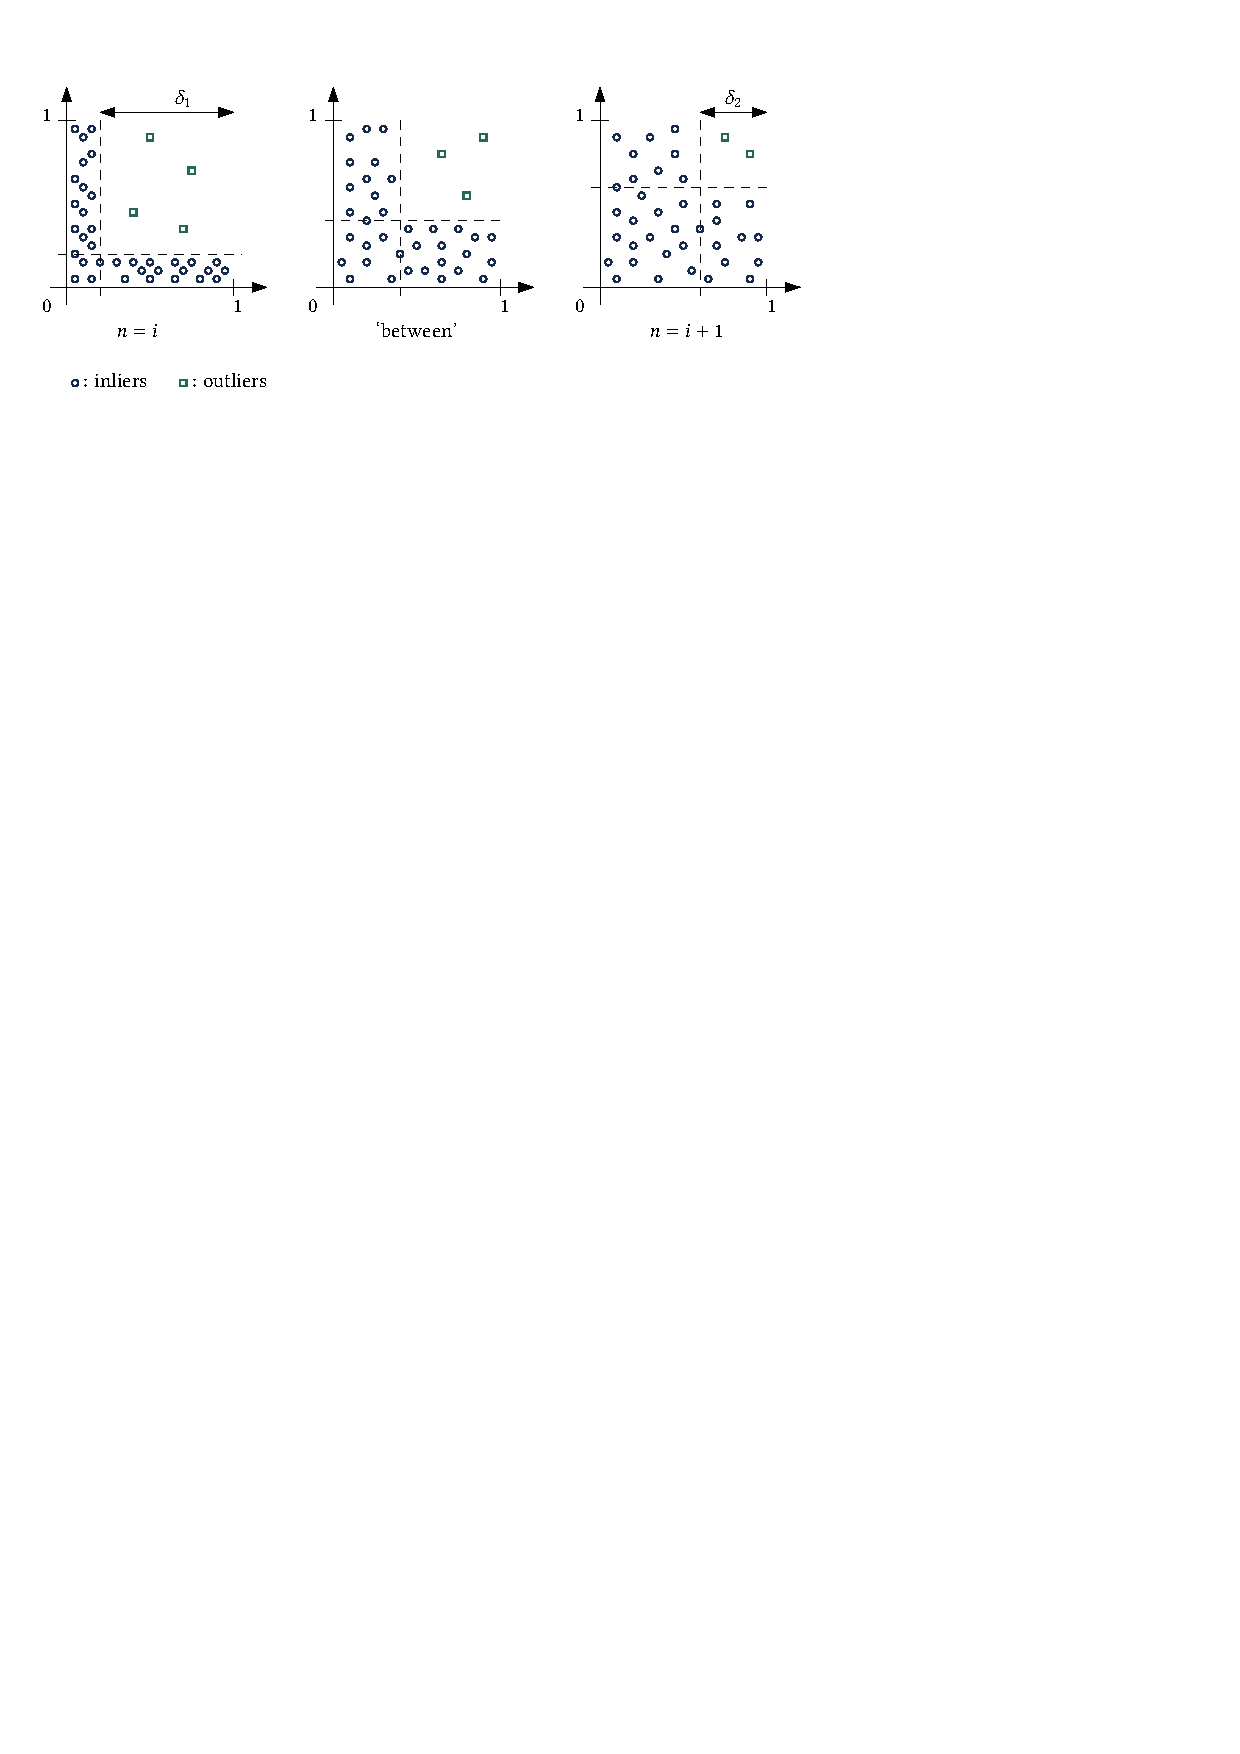
\includegraphics[width=\linewidth]{part4-figures/outliergeneration3-compressed.pdf}
	\caption{\acrshort{SGMRD}: Synthetic Benchmark Generation (Example).}
	\label{fig:SGMRD_generation}
\end{figure*} 

\subsection{Baselines and Competitors}

\subsubsection{Subspace Monitoring} 

Our goal is to assess how effectively \gls{SGMRD} can handle the trade-off between computational cost and monitoring quality. We compare \gls{SGMRD} to several alternative update strategies and against several baselines.
\begin{itemize}[noitemsep]
	\item \textsc{\gls{SGMRD}-S-TS} uses \acrfull{S-TS} as an update strategy. We let the efficiency parameter $\gls{eta^*}$ vary from $0.1$ to $0.9$.
	%\item \textsc{\gls{SGMRD}-STS-ADWIN} uses \acrfull{S-TS-ADWIN} as update strategy. We let the efficiency parameter $\gls{eta^*}$ vary from $0.1$ to $0.9$. We set the parameter of \acrshort{ADWIN}, $\delta = 0.1$, as recommended by the authors \cite{DBLP:conf/sdm/BifetG07}. 
	\item \textsc{\gls{SGMRD}-\acrshort{TS}} uses \gls{TS} as update strategy. This approach is similar to \textsc{\gls{SGMRD}-S-TS}, but the number of updates does not change over time.  
	\item \textsc{{SGMRD}-RD} uses a random (RD) update strategy. We update a single subspace per time step, chosen randomly from the current set of subspaces. 
	\item \textsc{{SGMRD}-GD} uses a greedy (GD) update strategy. We update a single subspace per time step and choose the subspace with the lowest quality in the current set. 
	\item \textsc{Batch} repeats the initialisation of \gls{SGMRD} periodically for every batch of data with size ${w}=1000$. 
	\item \textsc{Init} runs the initialisation and then keeps the same set of subspaces for the rest of the experiment (no update). 
	\item \textsc{Gold} repeats the initialisation of \gls{SGMRD} at every step. This baseline represents the highest level of quality that one can reach with this instantiation of \gls{SGMRD}, but it also is the most expensive configuration. 
	In fact, we can only afford to run it on the \textsc{Bioliq} data set.  
\end{itemize}

\subsubsection{Outlier Detection} 

We compare the results obtained with \textsc{\gls{SGMRD}-\gls{TS}} against the following outlier detectors: 
\begin{itemize}[noitemsep]
	\item \textsc{\acrshort{RS-Stream}} is an adaptation of the \textsc{\acrshort{RS-Hash}} \cite{DBLP:conf/icdm/SatheA16} outlier detector to the streaming setting, presented in \cite{DBLP:journals/kais/SatheA18}. It estimates the outlierness of each observation via randomised hashing over random projections. We reproduce the approach and use the default parameters recommended by the authors. 
	\item \textsc{\gls{LOF}} \cite{DBLP:conf/sigmod/BreunigKNS00} is a well-known outlier detector. We run it periodically and average the scores over a sliding window in the full space. We use the implementation from ELKI
	\cite{DBLP:journals/pvldb/SchubertKEZSZ15}, which profits from efficient index structures.% such as the R$^*$-tree. 
	\item \textsc{xStream} \cite{10.1145/3219819.3220107} is an ensemble outlier detector. \textsc{xStream} estimates densities via randomised ensemble binning  from a set of random projections. \textsc{xStream} declares the points lying in low density areas as outliers. We use the implementation from the authors  %\footnote{\url{https://github.com/cmuxstream/cmuxstream-core}} 
	with the recommended parameters. 
	\item \textsc{Stream\acrshort{HiCS}} \cite{becker2016concept} is an adaptation of \cite{DBLP:conf/icde/KellerMB12}. Based on a change detector, \textsc{Stream\acrshort{HiCS}} repeats the computation from \cite{DBLP:conf/icde/KellerMB12} on a data synopsis (so-called micro-clusters). We use the reference implementation  %\footnote{\url{https://github.com/vincentbecker/StreamHiCS}} 
	with default parameters. 
\end{itemize}

We average the scores obtained from each detector over a sliding window of size $w=1000$ for every $v=100$ time steps (cf.\ Section \ref{sec:downstream}). 
For approaches based on \gls{LOF}, such as ours, we repeat the computation with parameter $k \in \{1,2,5,10,20,50,100\}$ and report the best result in terms of  \acrshort{AUC}. 
The performance may vary widely w.r.t.\ this parameter; this is a well-known caveat of \gls{LOF} \cite{DBLP:journals/datamine/CamposZSCMSAH16}. 
We average every result from $10$ independent runs. 
Each approach runs single-threaded on a server with 20 cores at 2.2GHz and 64GB RAM. 
We implement our algorithms in Scala.% and we use Java Open-JDK 8.

\section{Results}

\subsection{Subspace Monitoring}

We first evaluate the quality of monitoring from \gls{SGMRD}. We set $\gls{w}=1000$, $v=2$ and $\gls{L}=1$, i.e., for each update strategy, \gls{SGMRD} only keeps the latest $1000$ observations, and, for any new two observations, 
\gls{SGMRD} attempts to replace one of the current subspaces. 

As we can see in Figure \ref{fig:SGMRD_SubspaceMonitoring_Quality}, both \textsc{\gls{SGMRD}-\gls{TS}} and \textsc{\gls{SGMRD}-RD} can keep the quality $\overline{Q}_{\gls{t}}$ close to that of \textsc{Gold}, our strongest and most expensive baseline. 
In the beginning, \textsc{\gls{SGMRD}-\gls{TS}} seems to perform slightly worse than \textsc{\gls{SGMRD}-RD}, but after some time (once \textsc{\gls{SGMRD}-\gls{TS}} has learned its update strategy), it tends to dominate \textsc{\gls{SGMRD}-RD}. 
We can see that \textsc{Batch} occasionally leads to the same quality as \textsc{Gold}, but the quality drops quickly between the update steps. 
\textsc{\gls{SGMRD}-GD} is not much better than \textsc{Init} (no monitoring). 

Figure \ref{fig:SGMRD_SubspaceMonitoring_Pseudoregret} confirms our observations: While the regret of \textsc{\gls{SGMRD}-\gls{TS}} is slightly worse than the one of \textsc{\gls{SGMRD}-RD} at the beginning, it becomes better afterwards. 
The other approaches lead to much higher regret. 
For larger step size $v$, we see that \textsc{\gls{SGMRD}-\gls{TS}} is superior to \textsc{\gls{SGMRD}-RD}. %For $v=1$, \textsc{SGMRD-RD} is slightly better. 
For smaller $v$, the environment does not change much between observations, and it is more difficult to learn which subspaces to update more frequently. 

\begin{figure}
	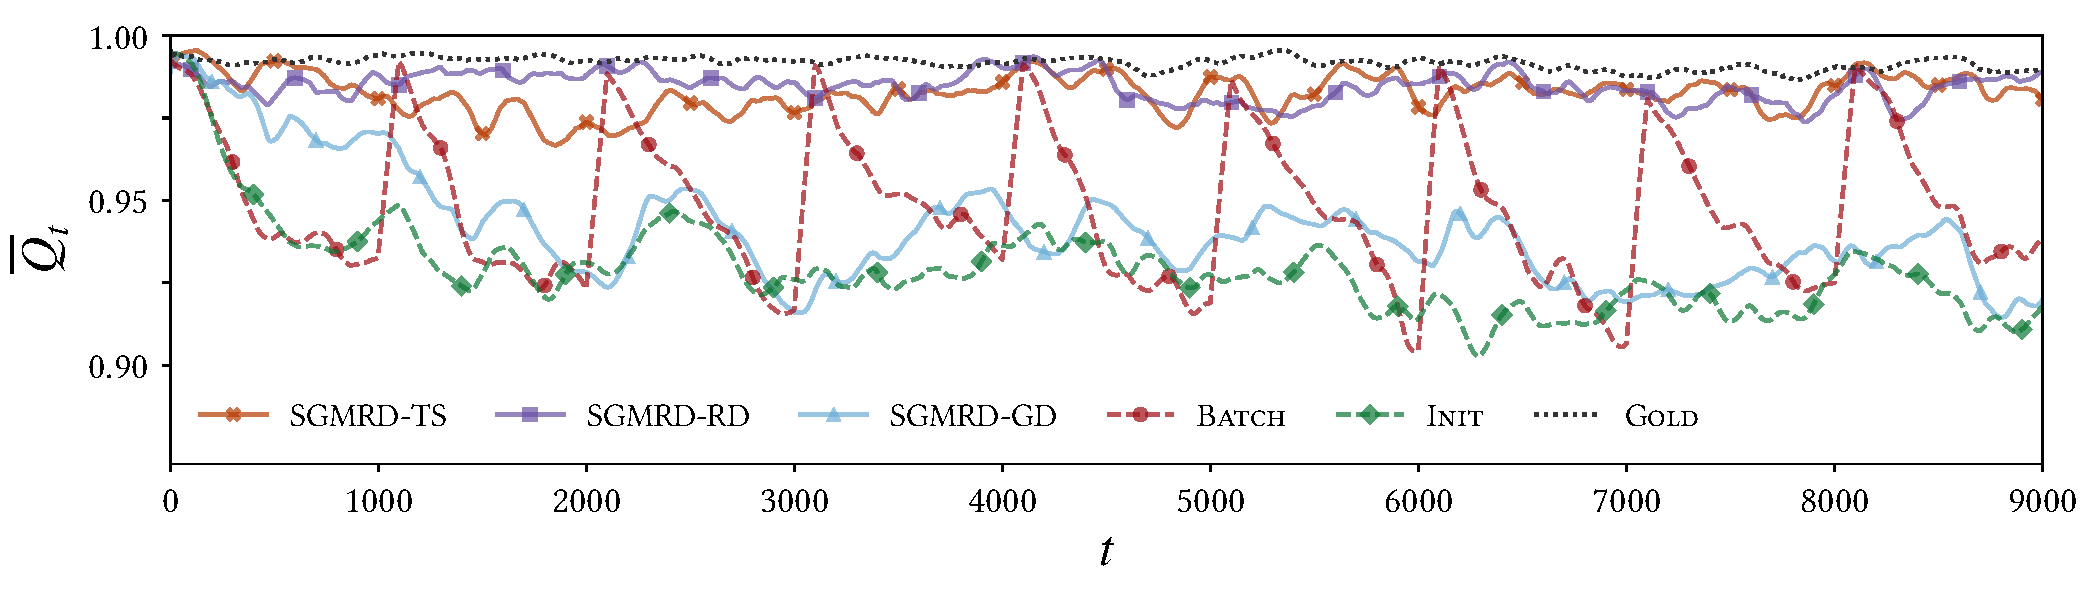
\includegraphics[width=\linewidth]{part4-figures/pyro_avgcontrast_step2_S_b_2-compressed.pdf}
	\caption{Average Quality at time $t$ (\textsc{Bioliq}, ${L}=1$, $v = 2$).} 
	\label{fig:SGMRD_SubspaceMonitoring_Quality}
\end{figure}

\begin{figure}
	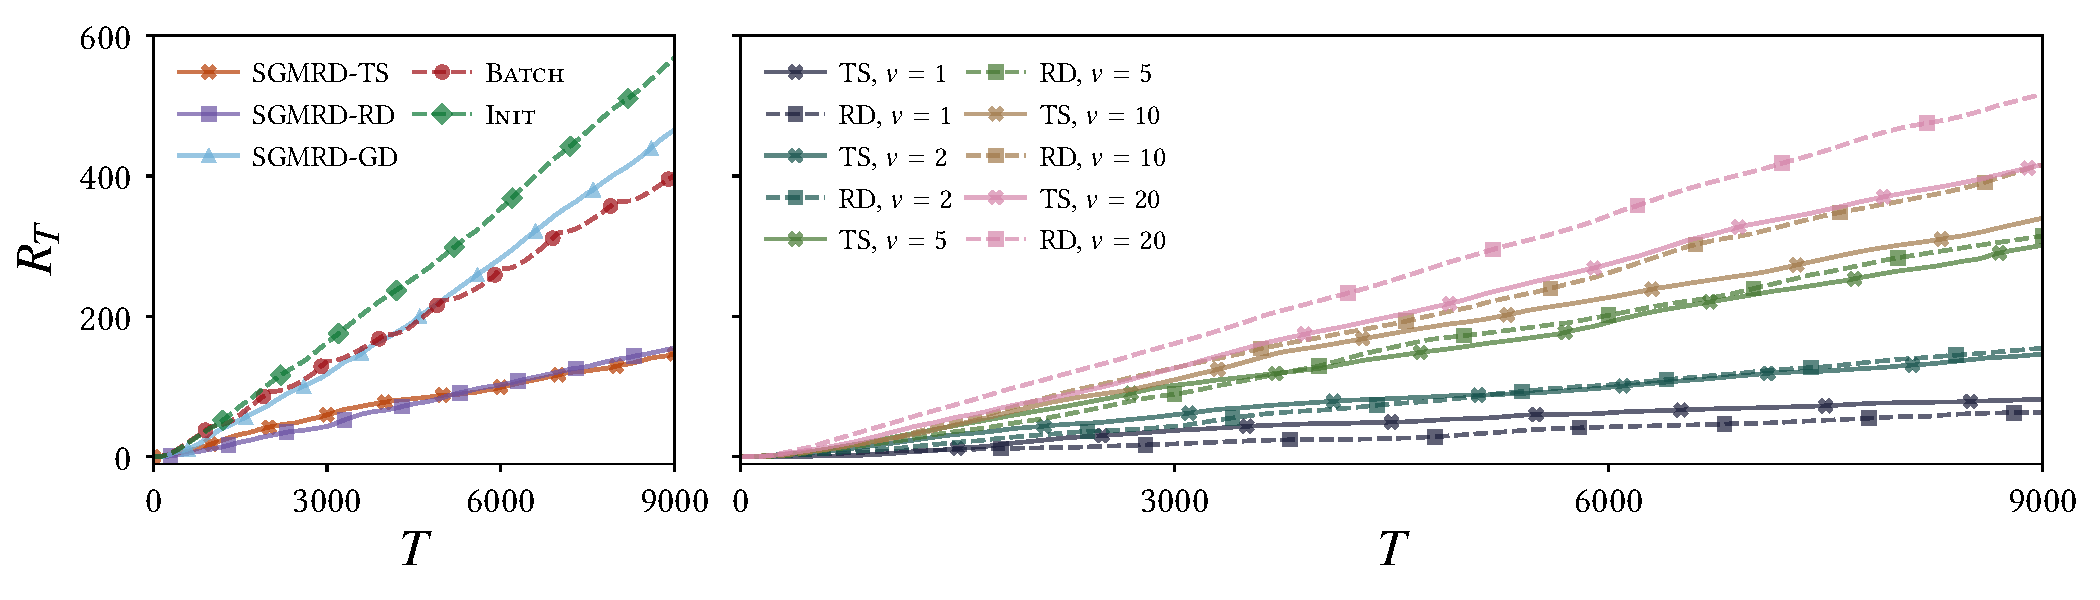
\includegraphics[width=\linewidth]{part4-figures/pyro_pseudoregret_step2_S_b_2-compressed.pdf}
	\caption{Regret up to $T$ (\textsc{Bioliq}, ${L}=1$, left: $v = 2$).} 
	\label{fig:SGMRD_SubspaceMonitoring_Pseudoregret}
\end{figure}

In Figure \ref{fig:SGMRD_UpdateFrequency}, the update frequencies show how the strategies differ. 
As expected, Random (RD) updates each subspace uniformly. Greedy (GD) tends to focus only on a few subspaces; most subspaces are never replaced, although they may become suboptimal as well. \acrshort{TS} focuses more on some subspaces, the ones requiring more frequent updates.

\begin{figure}
	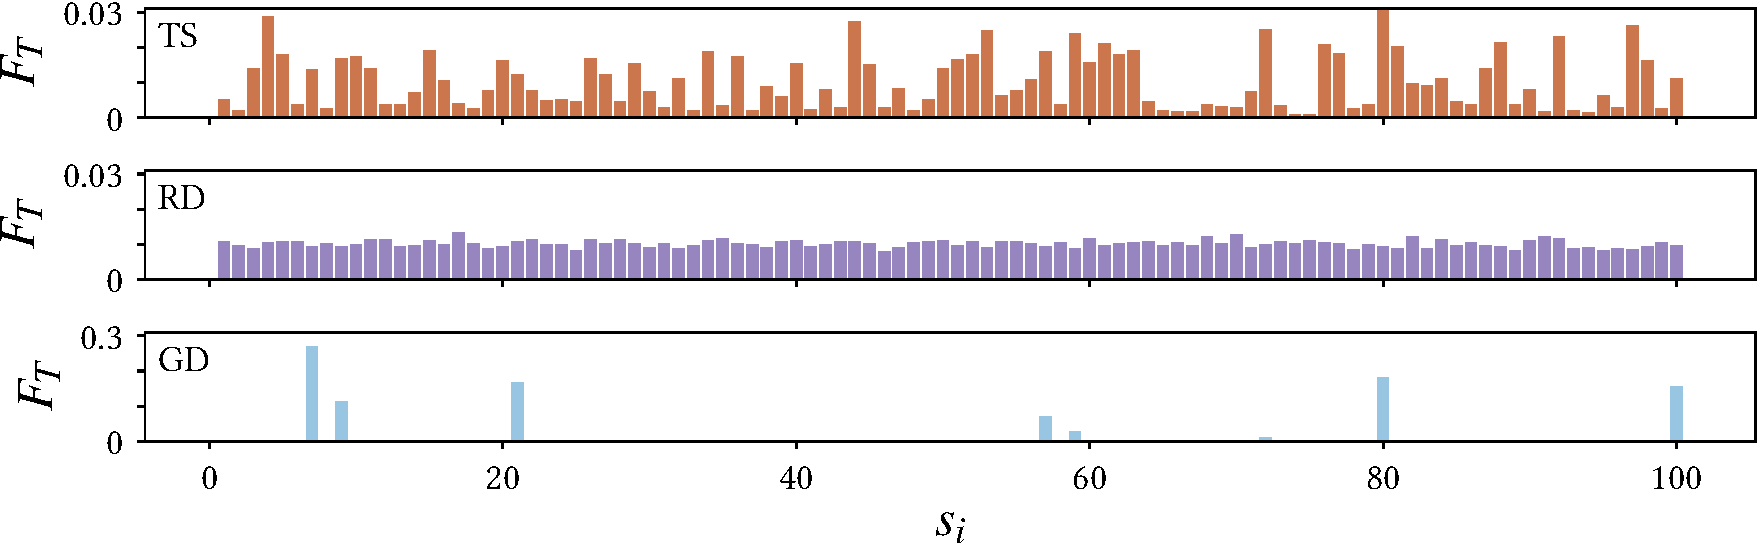
\includegraphics[width=\linewidth]{part4-figures/bioliq1_SGMRD_freq-crop-compressed.pdf}
	\caption{Frequency of update (\textsc{Bioliq}, $v = 2$, $L=1$).} 
	\label{fig:SGMRD_UpdateFrequency}
\end{figure} 

\begin{figure}
	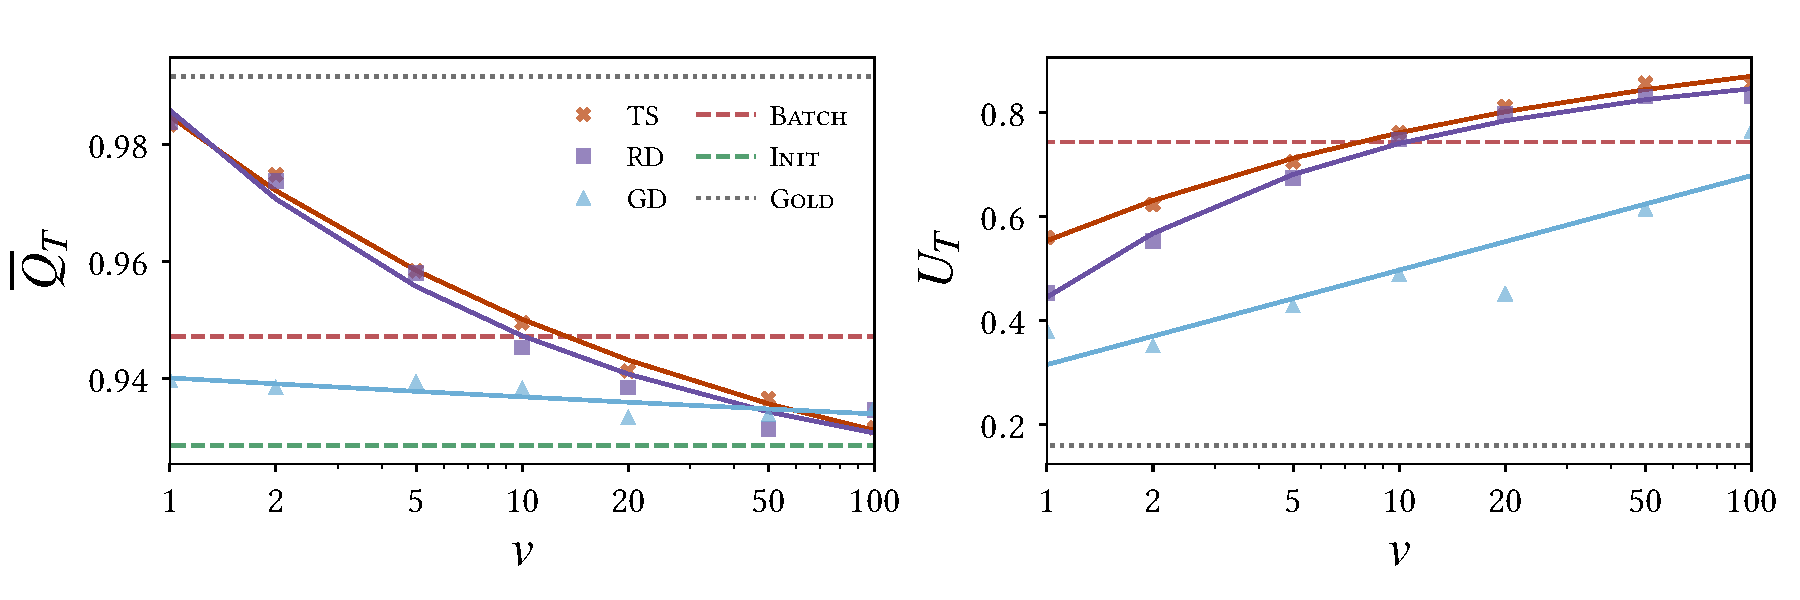
\includegraphics[width=\linewidth]{part4-figures/pyro_quality_success_step_3_S_b_2-compressed.pdf}
	\caption{Quality / Success Rate w.r.t.\ step size $v$ (\textsc{Bioliq}, $\gls{L}=1$).}
	\label{fig:SGMRD_QualityUpdateWRTstep}
\end{figure} 

\begin{figure}
	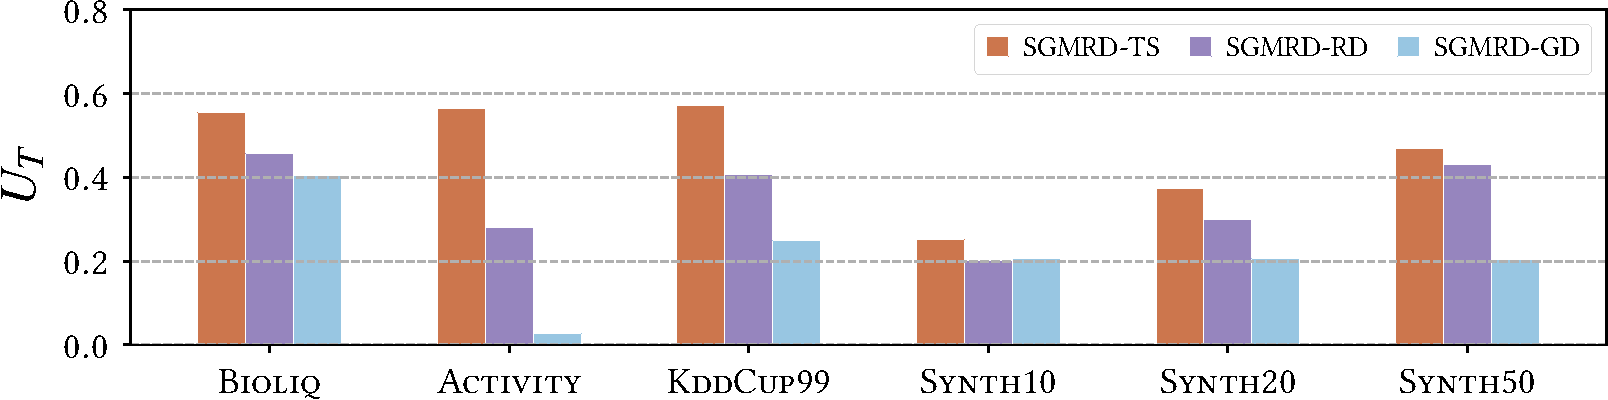
\includegraphics[width=\linewidth]{part4-figures/successratio-crop-compressed.pdf}
	\caption{Success Rate ($v = 1$, $\gls{L}=1$).} 
	\label{fig:SGMRD_SuccessRatio}
\end{figure} 

Figure \ref{fig:SGMRD_QualityUpdateWRTstep} shows that the average quality $\overline{Q}_{{T}}$ tends to decrease as we increase the update step $v$. However, the rate of successful updates $U_{{T}}$ (Equation \ref{eq:U_T}) increases. As $v$ increases, it is more likely for any subspace to become suboptimal. 
For \textsc{Batch}, $U_{{T}}$ is high, but the quality $\overline{Q}_{{T}}$ is low. 
We observe the opposite for \textsc{Gold}. %: The quality is very high, but rate of success very low. 
\gls{SGMRD} is a trade-off between these two extremes, and the strategy based on \acrfull{TS} appears superior to others, both w.r.t.\ $\overline{Q}_{{T}}$ and $U_{{T}}$. Figure \ref{fig:SGMRD_SuccessRatio} shows that our observations are not only valid for the \textsc{Bioliq} data set, but also for other benchmarks. \textsc{\gls{SGMRD}-\gls{TS}} consistently achieves a higher rate of successful updates than other approaches.  

\begin{figure}
	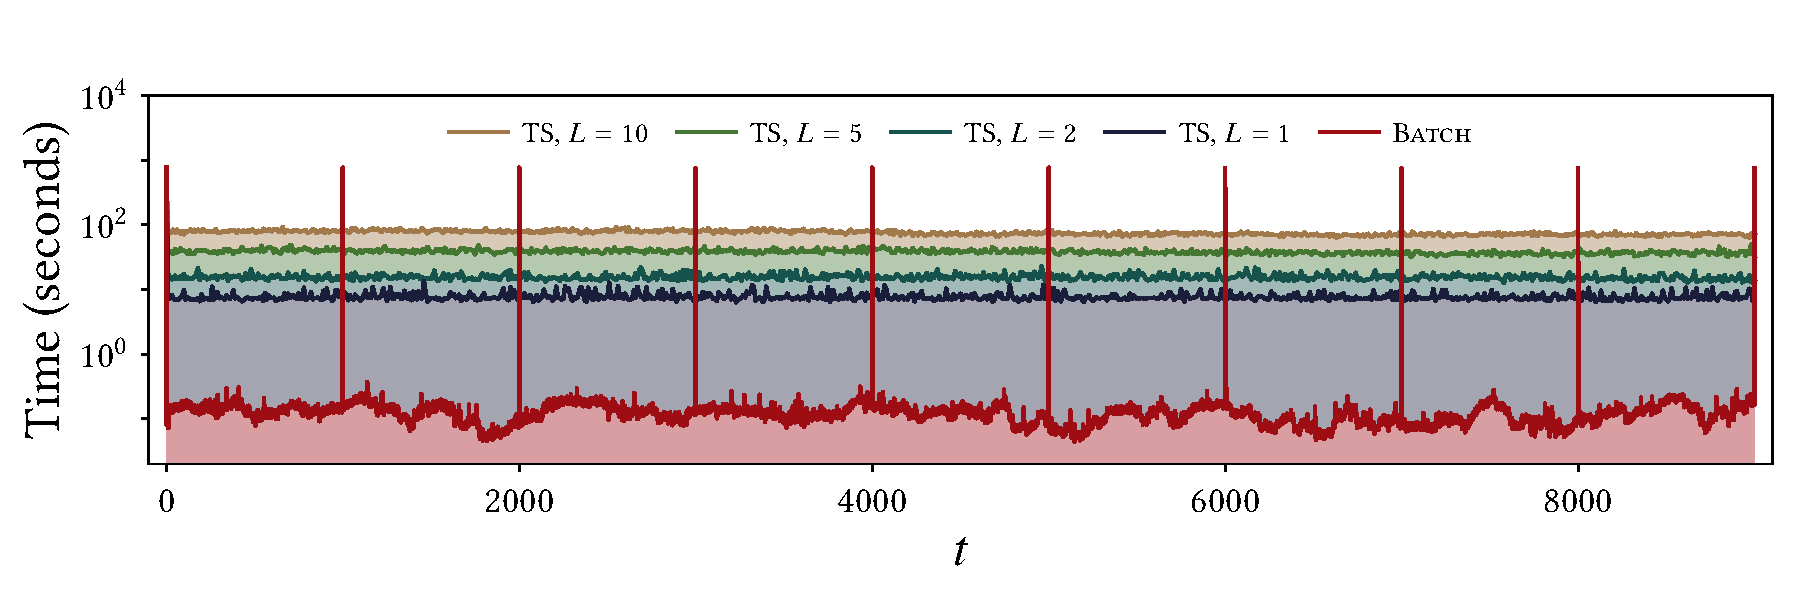
\includegraphics[width=\linewidth]{part4-figures/stream_runtime_S_b_2-compressed.pdf}
	\caption{Stream Processing Time (\textsc{Bioliq}, $v = 1$).}
	\label{fig:SGMRD_StreamProcessing}
\end{figure}

\begin{figure}
	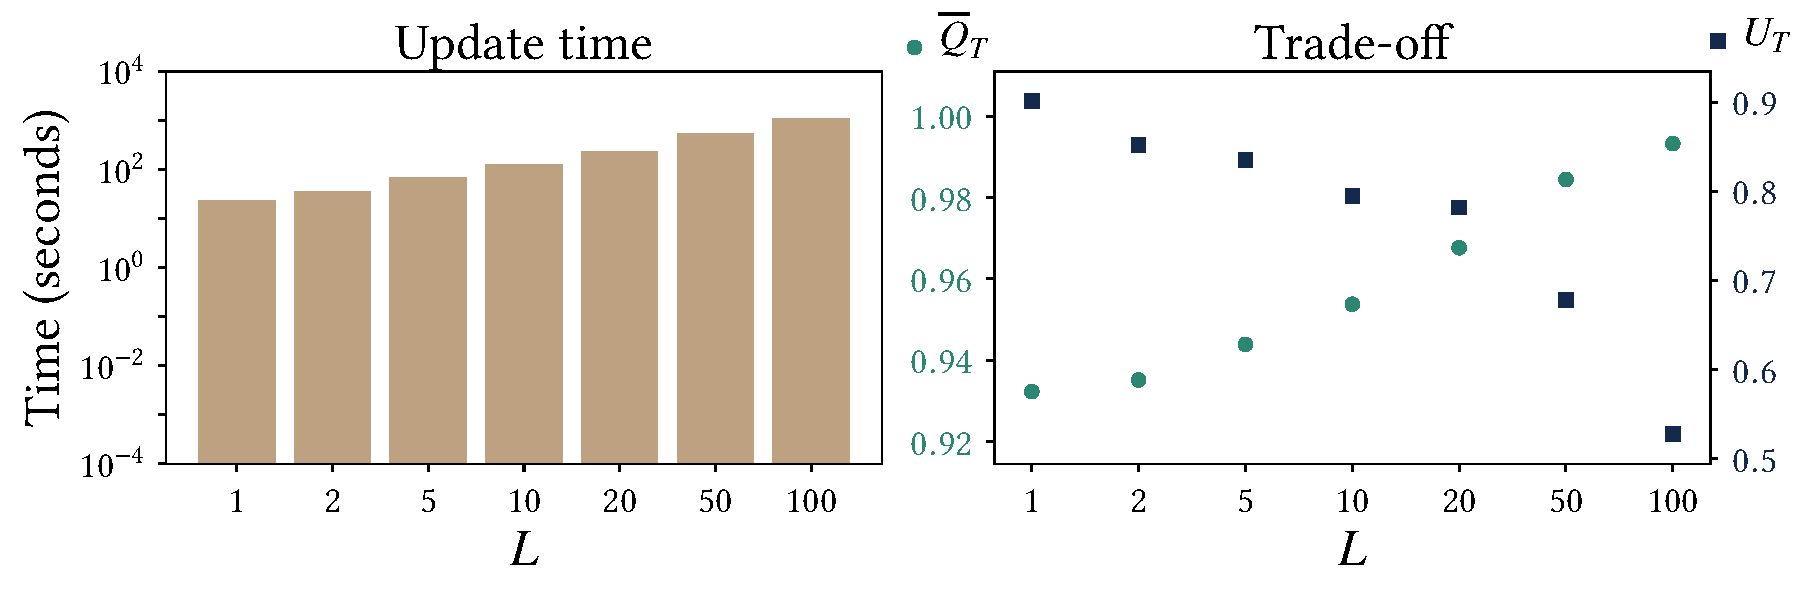
\includegraphics[width=\linewidth]{part4-figures/runtime_tradeoff_2-compressed.pdf}
	\caption{Quality/efficiency (\textsc{Bioliq}, \textsc{\gls{SGMRD}-\acrshort{TS}}, $v = 100$).} 
	\label{fig:SGMRD_Runtime}
\end{figure} 

Figure \ref{fig:SGMRD_StreamProcessing} highlights an important drawback of previous methods: The computation for batch-wise techniques is concentrated in a few discrete time steps. For stream mining, it is better to distribute computation uniformly over time. Computation-intensive episodes can lead to long response times of the system, and this contradicts the efficiency sought (\hyperlink{C1}{\textbf{C1}}) and anytime behaviour (\hyperlink{C4}{\textbf{C4}}). 
Besides this, the system becomes unable to adapt to the environment (\hyperlink{C3}{\textbf{C3}}) between the different episodes. 

Next, we set $v=100$ and let $\gls{L}$ vary to observe the trade-off between quality of the subspaces and the efficiency of the search in \textsc{\gls{SGMRD}-\gls{TS}} (see Figure \ref{fig:SGMRD_Runtime}). 
As $\gls{L}$ increases, %the cost associated with the index remains constant, but 
the cost of updating subspaces increases linearly. 
Similarly, the quality $Q_{\gls{T}}$ increases while the rate of successful updates $U_{\gls{T}}$ decreases.

\gls{S-MAB} algorithms are convenient tools for controlling this trade-off. Figure \ref{fig:SGMRD_Scaling} shows the number of plays/updates $\gls{L}_{\gls{t}}$ over time for \textsc{\gls{SGMRD}-S-TS}.  
As we can see, $\gls{L}_{\gls{t}}$ converges to an optimal amount of updates according to the efficiency criterion $\gls{eta^*}$ for \textsc{\gls{SGMRD}-S-TS}. 
Our scaling policy (\textsc{\gls{KL-S}}, Algorithm~\ref{S-TS}) scales up the number of updates/plays until we are confident that doing so violates the efficiency constraint. 
Note that, in non-static environments, we can further adapt the number of updates using \gls{ADWIN}, e.g., as in Section~\ref{non-static-adaptation}. 

\begin{figure}
	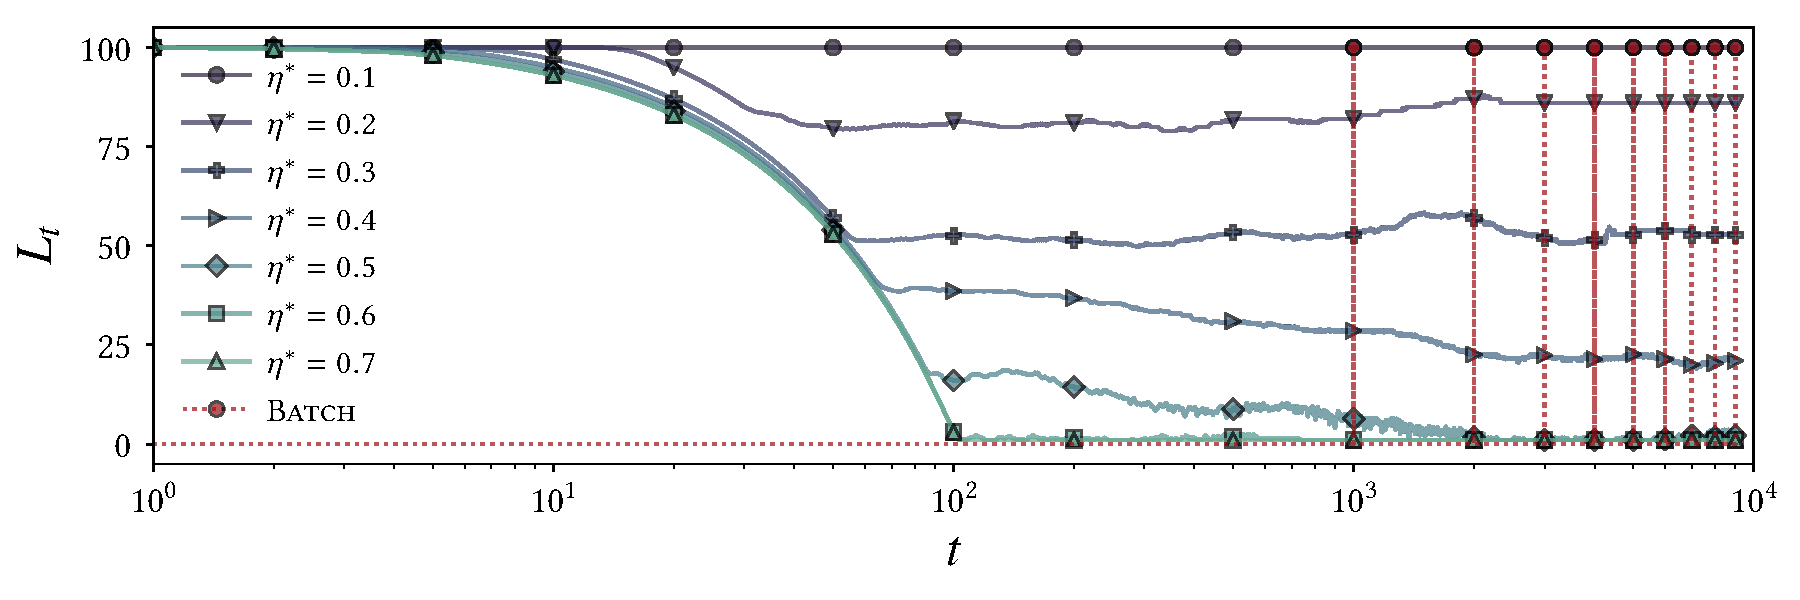
\includegraphics[width=\linewidth]{part4-figures/pyro_Lt_3_2-compressed.pdf}
	\caption{\gls{SGMRD}-\gls{S-TS}  (\textsc{Bioliq}, $v = 1$).} 
	\label{fig:SGMRD_Scaling}
\end{figure} 

\begin{table}
	\sisetup{detect-weight,mode=text}
	\renewrobustcmd{\bfseries}{\fontseries{b}\selectfont}
	\renewrobustcmd{\boldmath}{}
	\centering
	\caption{Comparison with Scaling Bandits (\textsc{Bioliq}, $v=1$).}
	\label{result:sgmrd_scaling}
	\addtolength{\tabcolsep}{-2.5pt}
	\centering
	\footnotesize
	\renewcommand{\arraystretch}{0.68}
	\begin{tabularx}{\textwidth}{@{}lXXXX|lXXXX@{}}
		\toprule
		\textbf{Baseline} & \textbf{$L_{\gls{T}}$} & \textbf{$\overline{Q}_{\gls{T}}$} & \textbf{$U_{\gls{T}}$} & \textbf{$R_{\gls{T}}/T$} & \textbf{\gls{SGMRD}-\gls{S-TS}} & \textbf{$L_{\gls{T}}$} & \textbf{$\overline{Q}_{\gls{T}}$} & \textbf{$U_{\gls{T}}$}  & \textbf{$R_{\gls{T}}/T$}  \\ \midrule
		\textbf{\gls{TS}}    & 1     & 95.43       & 0.61    &  3.74   & $\eta^*=0.1$         & 100.00 	  & 99.45 	    & 0.16  &  0.09   \\
		\textbf{RD}    & 1           & 95.20       & 0.54    &  3.97   & $\eta^*=0.2$         & 74.13 	  & 99.19 	    & 0.20  &  0.08   \\
		\textbf{GD}    & 1           & 93.72       & 0.43    &  5.45   & $\eta^*=0.3$         & 54.48 	  & 99.22 	    & 0.29  &  0.06    \\
		\textbf{Batch} & --          & 95.16       & 0.81    &  4.01   & $\eta^*=0.4$         & 36.78 	  & 99.33 	    & 0.37  &  0.78    \\
		\textbf{Init}  & --          & 92.50       & --       &  6.67   & $\eta^*=0.5$         & 5.73 	  & 98.79 	    & 0.46  &  2.46     \\
		\textbf{Gold}   & 100         & 99.16       & 0.16    &   & $\eta^*=0.6$         & 1.68 	  & 97.62 	    & 0.53  &  2.81   \\
		&          &          &         					  &   & $\eta^*=0.7$         & 1.58       & 97.68 	    & 0.53  &  2.26   \\
		&          &          &         					  &	  & $\eta^*=0.8$         & 1.57 	  & 97.75 	    & 0.55  &  2.32    \\
		&          &          &         					  &   & $\eta^*=0.9$         & 1.56 	  & 97.31 	    & 0.55  &  2.59    \\ \bottomrule
	\end{tabularx}
\end{table}

As we can see in Table \ref{result:sgmrd_scaling}, \textsc{\gls{SGMRD}-\gls{TS}} has the highest quality after \textsc{Gold}, the best success rate $U_{\gls{T}}$ after \textsc{Batch} and the smallest average regret among the baselines. It is interesting to see that the Scaling Bandits consistently lead to higher quality and smaller regret. Also, \textsc{\gls{SGMRD}-\gls{S-TS}} adjusts the number of plays so that $U_{\gls{T}}$ approximately matches $\gls{eta^*}$. Naturally, this only works up to a certain point, depending on the distribution of rewards in the environment. %Also, our algorithm must update at least one subspace at each step, with here $v=1$. 

In conclusion, the experiments show that \gls{SGMRD} is a useful tool to monitor high-quality subspaces over time, and it is highly versatile. Based on the available hardware, users can set the number of plays per round, as with \textsc{\gls{SGMRD}-\gls{TS}}, to obtain the highest quality from this budget. If the computation is no bottleneck, then users can set an efficiency threshold, which leads to an adequate use of resources for subspaces monitoring.     

In the next section, we show that \textsc{\gls{SGMRD}-\gls{TS}} helps to detect outliers and compare the results with state-of-the-art outlier detectors for data streams.  

\subsection{Outlier Detection}

\begin{table}[]
	\sisetup{detect-weight,mode=text}
	\renewrobustcmd{\bfseries}{\fontseries{b}\selectfont}
	\renewrobustcmd{\boldmath}{}
	\centering
	\caption{Outlier Detection Performance.}
	\label{result:sgmrd_outlierdetection}
	\footnotesize
	\renewcommand{\arraystretch}{0.68}
	\begin{tabularx}{\textwidth}{@{}XXllllllll@{}}
		\toprule
		Benchmark & Approach       & AUC            & AP             & P1\%           & P2\%           & P5\%           & R1\%           & R2\%           & R5\%           \\ \midrule
		\textsc{Activity}  & \textsc{\textbf{\gls{SGMRD}}} & \textbf{97.32} & \textbf{85.39} & \textbf{94.59} & \textbf{94.83} & \textbf{94.24} & \textbf{9.44}  & \textbf{18.97} & \textbf{47.10} \\
		& \textsc{\gls{LOF}}      & 93.93          & 61.80          & 74.32          & 64.72          & 64.03          & 7.42           & 12.94          & 32.00          \\
		& \textsc{Stream\gls{HiCS}}     & 88.52          & 47.38          & 70.72          & 54.61          & 51.89          & 7.06           & 10.92          & 25.93          \\
		& \textsc{\gls{RS-Stream}}      & 95.95          & 68.23          & 71.62          & 72.58          & 75.00          & 7.15           & 14.52          & 37.48          \\
		& \textsc{xStream}        & 77.71          & 20.41          & 3.60           & 10.14          & 16.31          & 0.36           & 2.02           & 8.13           \\ \midrule
		\textsc{KddCup99}  & \textbf{\gls{SGMRD}} & \textbf{69.98} & \textbf{10.29} & \textbf{0.00}  & \textbf{0.20}  & \textbf{0.56}  & \textbf{0.00}  & \textbf{0.06}  & \textbf{0.39}  \\
		& \textsc{LOF}      & 65.07          & 9.57           & 0.00           & 0.00           & 0.08           & 0.00           & 0.00           & 0.06           \\
		& \textsc{Stream\gls{HiCS}}     & 57.11          & 7.89           & 0.00           & 0.00           & 0.08           & 0.00           & 0.00           & 0.06           \\
		& \textsc{\gls{RS-Stream}}      & 43.21          & 5.73           & 0.00           & 0.00           & 0.08           & 0.00           & 0.00           & 0.06           \\
		& \textsc{xStream}        & 52.70          & 8.23           & 0.00           & 0.20           & 0.08           & 0.00           & 0.06           & 0.06           \\ \midrule
		\textsc{Synth10}   & \textbf{\gls{SGMRD}} & \textbf{92.70} & \textbf{59.93} & \textbf{50.00} & \textbf{26.00} & \textbf{12.00} & \textbf{58.14} & \textbf{60.47} & \textbf{69.77} \\
		& \textsc{\gls{LOF}}      & 88.77          & 31.44          & 33.00          & 18.50          & 10.40          & 38.37          & 43.02          & 60.47          \\
		& \textsc{Stream\gls{HiCS}}     & 88.81          & 31.16          & 33.00          & 19.00          & 10.40          & 38.37          & 44.19          & 60.47          \\
		& \textsc{\gls{RS-Stream}}      & 71.23          & 1.87           & 0.00           & 0.00           & 2.80           & 0.00           & 0.00           & 16.28          \\
		& \textsc{xStream}        & 68.51          & 2.58           & 5.00           & 3.00           & 4.00           & 5.81           & 6.98           & 23.26          \\ \midrule
		\textsc{Synth20}   & \textbf{\gls{SGMRD}} & \textbf{85.05} & \textbf{41.19} & \textbf{36.00} & \textbf{19.50} & \textbf{9.20}  & \textbf{40.91} & \textbf{44.32} & \textbf{52.27} \\
		& \textsc{\gls{LOF}}      & 72.55          & 5.57           & 8.00           & 6.00           & 4.40           & 9.09           & 13.64          & 25.00          \\
		& \textsc{Stream\gls{HiCS}}     & 71.71          & 5.37           & 8.00           & 6.00           & 4.00           & 9.09           & 13.64          & 22.73          \\
		& \textsc{\gls{RS-Stream}}      & 48.39          & 0.80           & 0.00           & 0.00           & 0.00           & 0.00           & 0.00           & 0.00           \\
		& \textsc{xStream}        & 63.64          & 1.58           & 1.00           & 1.50           & 2.20           & 1.14           & 3.41           & 12.50          \\ \midrule
		\textsc{Synth50}   & \textbf{\gls{SGMRD}} & \textbf{75.87} & \textbf{31.27} & \textbf{27.00} & \textbf{16.00} & \textbf{7.60}  & \textbf{33.33} & \textbf{39.51} & \textbf{46.91} \\
		& \textsc{\gls{LOF}}      & 61.38          & 1.08           & 0.00           & 0.50           & 0.60           & 0.00           & 1.23           & 3.70           \\
		& \textsc{Stream\gls{HiCS}}     & 63.90          & 12.00          & 11.00          & 6.00           & 3.40           & 13.58          & 14.81          & 20.99          \\
		& \textsc{\gls{RS-Stream}}      & 46.52          & 0.73           & 0.00           & 0.00           & 0.00           & 0.00           & 0.00           & 0.00           \\
		& \textsc{xStream}        & 48.43          & 0.90           & 1.00           & 0.50           & 1.40           & 1.23           & 1.23           & 8.64           \\ \bottomrule
	\end{tabularx}
\end{table} 

\begin{figure}
	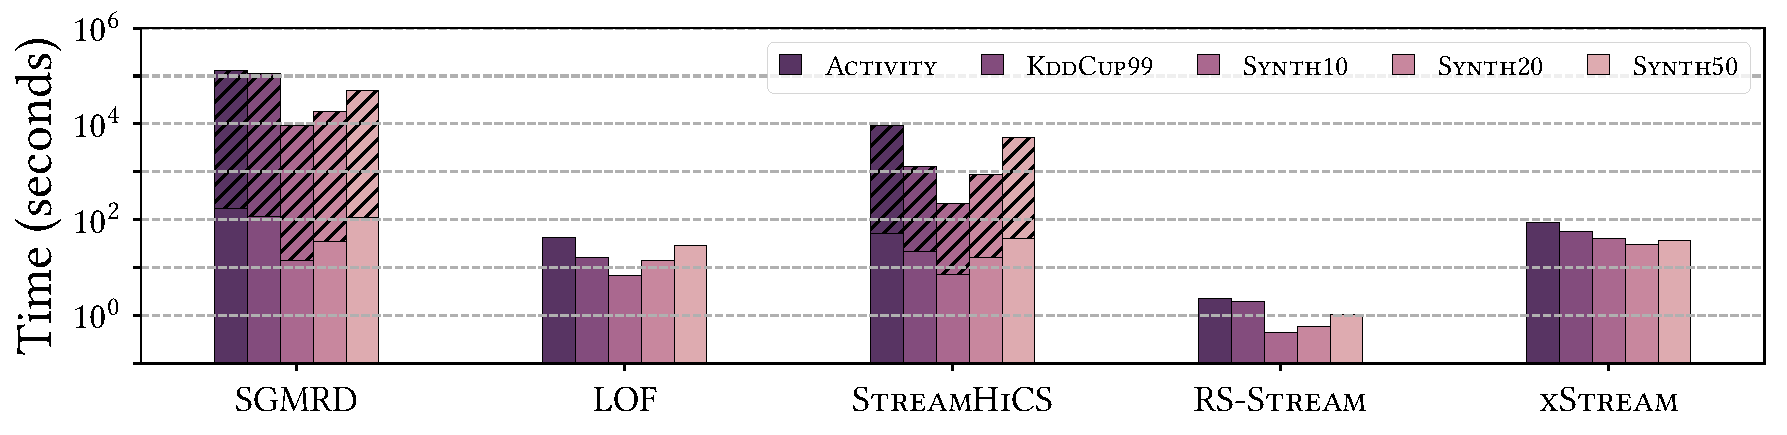
\includegraphics[width=\linewidth]{part4-figures/runtime-2-2-compressed.pdf}
	\caption{Outlier Detection Time (hatched area: search time).} 
	\label{fig:SGMRD_OutlierDetectionRuntime}
\end{figure} 

We leverage the subspaces obtained from \textsc{\gls{SGMRD}-\gls{TS}} to detect outliers, as in Section \ref{sec:downstream}. We set $\gls{w}=1000$, $v=1$ and $\gls{L}=1$. Table \ref{result:sgmrd_outlierdetection} shows the results. \textsc{\gls{SGMRD}} clearly leads to the best results w.r.t.\ each benchmark. It is interesting to see that \gls{LOF} turns out to be our most competitive baseline and often outperforms our competitors. 

In Figure \ref{fig:SGMRD_OutlierDetectionRuntime}, we can see that our competitors, in particular \textsc{\acrshort{RS-Stream}} and \textsc{xStream}, are much faster than \textsc{\gls{SGMRD}}, but they often are not much better than random guessing. 
Most of the computation required by \textsc{\gls{SGMRD}} and \textsc{Stream\acrshort{HiCS}} is due to the search. 
Nonetheless, one may reduce the required computation with \textsc{\gls{SGMRD}}, e.g., increase $v$, without decreasing detection quality by much. 

%While our experiments show the potential of \textsc{SGMRD} for outlier detection, we may expect similar benefits for any other knowledge discovery tasks in data streams. 

\section{Discussion}

Finding interesting subspaces is fundamental to any step of the \gls{KDD} process. We have proposed a new method, \gls{SGMRD}, to bring subspace search to streams. Our approach leverages our previous contributions: on the one hand, we use \gls{MCDE} (Chapter \ref{chapter:MCDE}) to estimate the quality of subspaces. We can monitor the resulting estimates efficiently, thanks to our incremental index structure. On the other hand, \gls{SGMRD} learns an update strategy to determine the subspaces to update at each time step. We use bandit theory and \gls{S-MAB} algorithms (Chapter \ref{chapter:S-MAB}) to address the trade-off between the quality of monitoring and the required computation. 

Our experiments not only show that \gls{SGMRD} leads to efficient monitoring of subspaces, but also to state-of-the-art results w.r.t.\ downstream Knowledge Discovery tasks, such as outlier detection. One may expect similar benefits for other mining tasks on streams. 

An administrator can control monitoring via two parameters: the number of plays per round $L$ and the step size $v$. While \gls{SGMRD} can leverage \gls{S-MAB} to decide the appropriate number of updates per steps $L$ automatically, finding the most adequate step size $v$ for a specific problem is not trivial. 
In future work, it would be interesting to extend the \gls{S-MAB} framework, such that the underlying bandit algorithm can not only decide which arms and how many arms to play, but also whether to play at all.  

Next, we focus on a more specific Knowledge Discovery task: mining text outliers. This task is more challenging than typical outlier detection tasks, so we first address it in the static setting. Nonetheless, it is easy to see how \gls{SGMRD} could help to transfer the problem to the streaming setting, as we discuss in our future work (Chapter \ref{chapter:futurework}). 

\chapter{Mining Text Outliers} 
\glsresetall
\label{chapter:textoutlier}

The results from this chapter have been published as follows: 
\begin{itemize}[noitemsep]
	\item \fullcite{DBLP:conf/ssdbm/FoucheMGZBH20}
\end{itemize}
\textbf{Keywords:} Text Mining; Anomaly Detection; Data Cleaning; Nearest-Neighbour Search

\section{Chapter Overview}

Nowadays, it is common to classify collections of documents into (human-generated, domain-specific) directory structures, such as email or document folders. But documents may be classified wrongly, for a multitude of reasons. Then they are outlying w.r.t.\ the folder they end up in. Orthogonally to this, and more specifically, two kinds of errors can occur: (O) Out-of-distribution: the document does not belong to any existing folder in the directory; and (M) Misclassification: the document belongs to another folder. It is this specific combination of issues that we address in this article, i.e., we mine text outliers from massive document directories, considering both error types (see also the motivations in Section~\ref{sec:textoutlierprelim}). We make the following contributions:  

\textbf{We explore the problem of text outlier detection in document directories}. The task is challenging because text can be outlying in numerous ways, and directories are domain-specific. At the same time, text outliers fall into two categories: Types~O/M. 
To our knowledge, we are first to propose an integrated outlier detection framework for text documents that builds on this conceptual distinction. 

\textbf{We propose a new proximity-based approach to detect text outliers}, which we name \gls{kj-NN}. Our approach leverages similarities of documents and phrases, based on state-of-the-art embedding methods \cite{meng2019spherical}, to detect both Type~O/M outliers. By extracting semantically relevant labels and the documents similar to each outlier, it also supports interpretability. 

\textbf{We introduce a `self-supervision' mechanism} to make our approach more robust. Our idea is to weigh each decision by the relevance of neighbouring documents. A document is said to be relevant w.r.t.\ a given class when its semantics, characterised by its closest phrases in the embedding space, is representative of its class. 

\textbf{We conduct extensive experiments} to compare our method to competitors and provide example outputs. The experiments show that our approach improves the current state of the art by a large margin while delivering interpretable results.

\textbf{We release our source code on GitHub}\footnote{\url{https://github.com/edouardfouche/MiningTextOutliers}}, together with our benchmark data, 
to ensure the reproducibility of our experiments. 
\enlargethispage{\baselineskip} % allow one more line (exceptionally) https://tex.stackexchange.com/questions/32112/squeeze-some-more-lines-on-the-current-page

\section{The \acrshort{kj-NN} Algorithm}
\label{sec:framework}

\begin{figure*}
	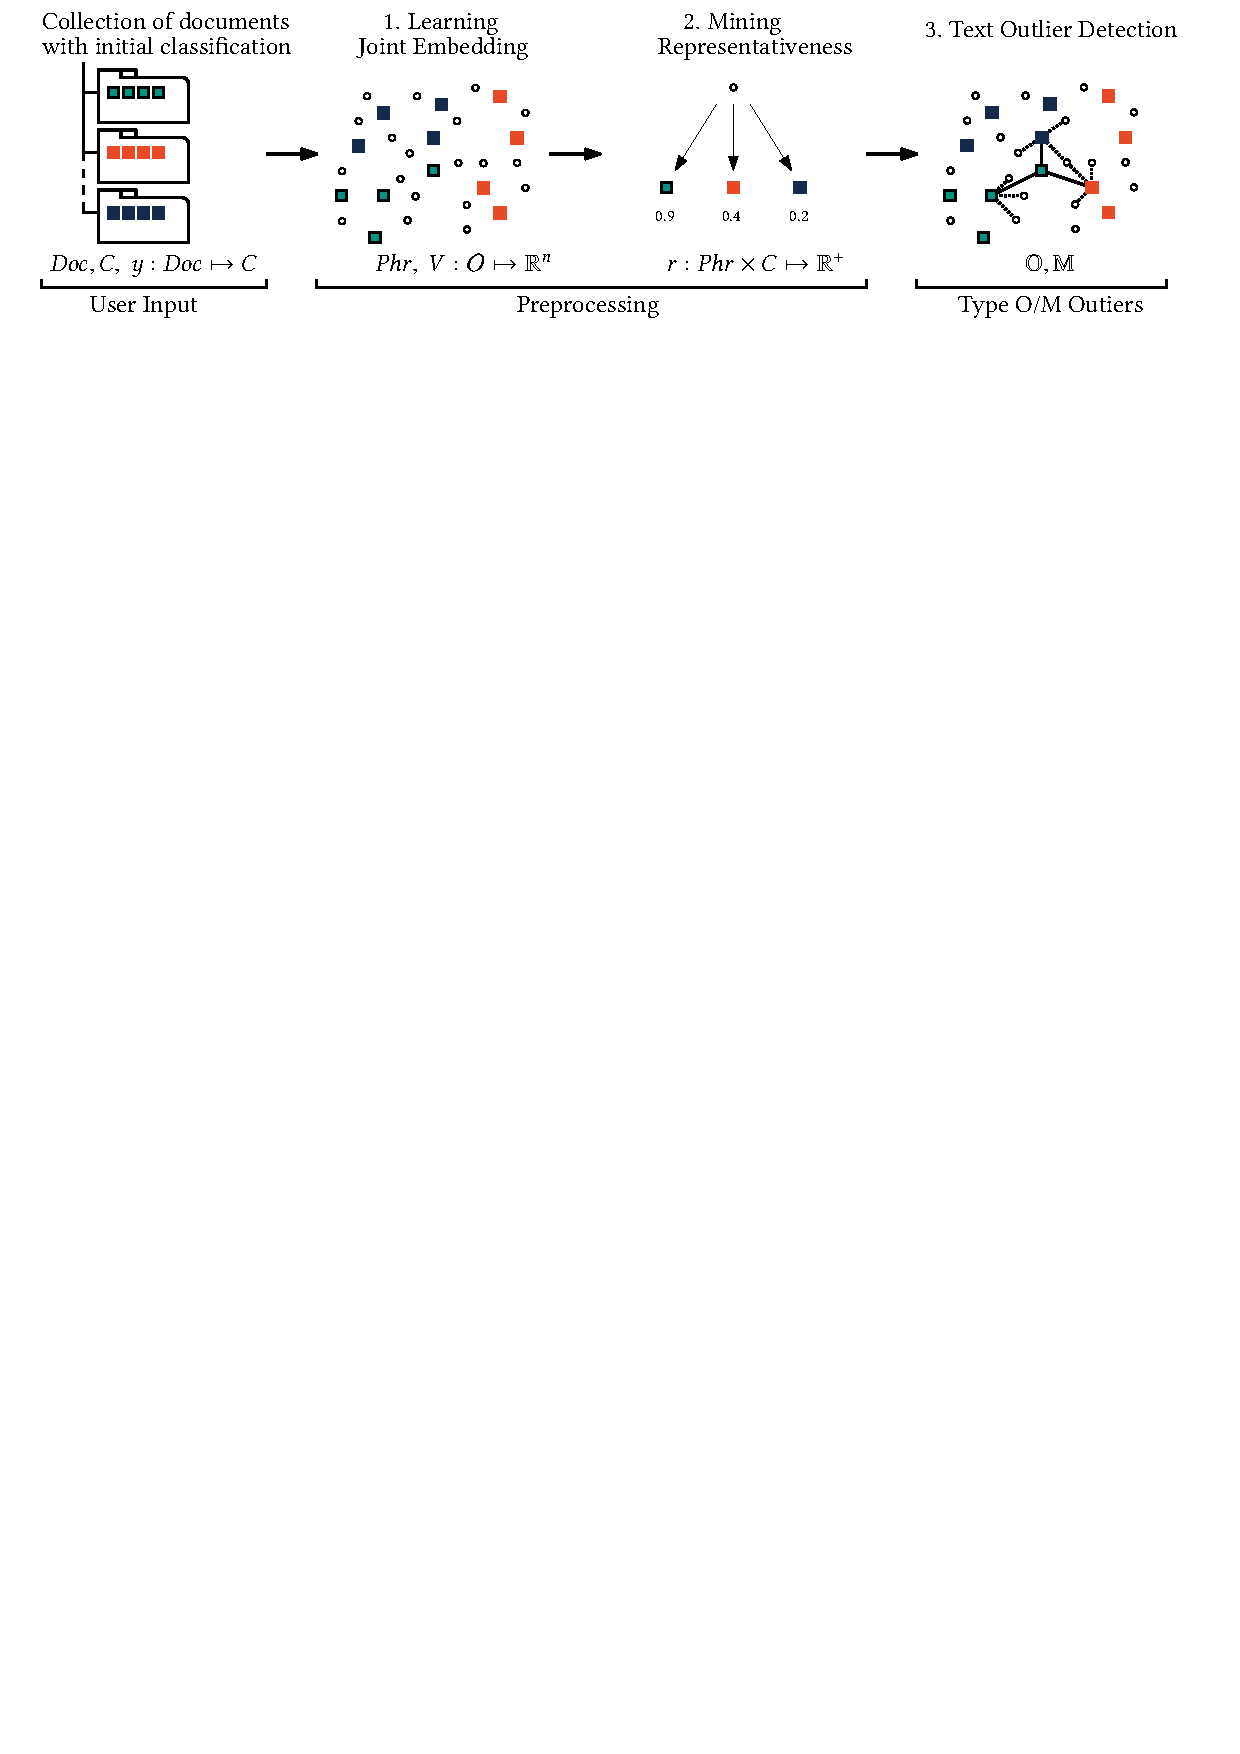
\includegraphics[width=\linewidth]{part4-figures/workflow5-compressed.pdf}
	\caption{Our Framework: A High-Level Overview. In the illustrations, squares are documents and dots are phrases.}
	\label{fig:workflow}
\end{figure*} 

\subsection{Our Framework}
\label{sec:kjNNframework}

Figure \ref{fig:workflow} provides a high-level overview of our framework. We assume as input a collection of documents $\gls{Doc}$, with an initial but imperfect classification $\gls{y}: \gls{Doc} \mapsto \gls{C}$ provided by the user. Squares stand for documents, and the colours represent their initial class. Documents are composed of phrases, represented in turn as dots. We design our framework in three steps: 

\textbf{1. Learning Joint Embedding:} Text outlier detection relies on textual similarity/dissimilarity measures, which can be effectively captured by %text 
embeddings. We segment the phrases $\gls{Phr}$ from every document using AutoPhrase \cite{DBLP:journals/tkde/ShangLJRVH18} and obtain the phrase and document embeddings $\gls{V}: \gls{O} \mapsto \mathbb{R}^n$ in a joint spherical space via \gls{JoSE}. 

The benefits of using \gls{JoSE} are %mainly 
twofold: (1) \gls{JoSE} trains document %embeddings
and phrase embeddings jointly in the same space, where text similarity between phrases and documents can be directly derived. (2) \gls{JoSE} captures directional similarity by training in the spherical space, which characterises textual similarity more effectively than Euclidean embeddings. 

\textbf{2. Mining Representativeness:} We estimate the representativeness of each phrase for each class, based on the initial classification. The representative phrases for a class are indicative of the semantics of documents. 
As in \cite{DBLP:journals/debu/TaoZYWCKVH16}, we define the representativeness as a function of three criteria: 
\begin{itemize}[noitemsep]
    \item \textbf{Integrity:} A phrase with high integrity in a given corpus is meaningful, understandable and of high quality. 
    \item \textbf{Popularity:} A phrase is popular in a given class if it has many occurrences. 
    \item \textbf{Distinctiveness:} A phrase is distinctive if it distinguishes a class from others.
\end{itemize}
For each phrase $\gls{p} \in \gls{Phr}$ and class $\gls{c} \in \gls{C}$, we estimate the integrity $\mathit{int}(\gls{p},\gls{c}) \in [0,1]$, popularity $\mathit{pop}(\gls{p},\gls{c}) \in \mathbb{R}^+$ and the distinctiveness $\mathit{disti}(\gls{p},\gls{c}) \in [0,1]$ as described in \cite{DBLP:series/synthesis/2019Zhang}. The representativeness is the product of those three criteria:
\begin{align}
    \gls{r}(\gls{p},\gls{c}) = \mathit{int}(\gls{p},\gls{c}) \cdot \mathit{pop}(\gls{p},\gls{c}) \cdot \mathit{disti}(\gls{p},\gls{c}).
\end{align}
The idea is that, even if each class may contain ambiguous documents or erroneous labels, these are `rare', so the impact on the estimation of representativeness is low. Our experiments show that our method is robust against %large shares of 
erroneous labels.
%EF: Hm. maybe this calls for experiments.... We could measure Jaccard coefficient between the top-k for each class with various amount of noise. 
%EF: Prof. Han suggested some improvements for this step (bootstraping). Experiment shows that results improve, but it is marginal.

\textbf{3. Text Outlier Detection:} We introduce \gls{kj-NN}, an outlier detector inspired by the well-known k-NN classifier \cite{fix1951discriminatory}. The main novelty is that inferring the class of each element (document) does not only base on the class of its $k$ nearest documents but also on their relevance. 
We estimate the relevance of a document as the average representativeness of its $j$ nearest sub-elements (phrases) for its class. 
If a document $\gls{d}$ is closer to documents which are (i) relevant and (ii) from another single class, then $\gls{d}$ likely is a Type~M outlier. 
On the other hand, if $\gls{d}$ is similarly close to relevant documents of various classes, then $\gls{d}$ likely is a Type~O outlier. This final step yields two ranked lists $\mathbb{O}$ and $\mathbb{M}$ of outliers for Type~O and Type~M, respectively.

In our approach, self-supervision consists of estimating the relevance of the original label, recognising that less relevant labels must have a lower influence on our predictions. 
The rationale is to perceive irrelevant documents as such because they either were misclassified or have ambiguous semantics. 

In the next section, we present the technical details of our outlier detector. We first provide a Bayesian formalisation, then describe the practical implementation of \gls{kj-NN}. 

\subsection{Formalisation}

We define the $k$ nearest documents and the $j$ nearest phrases of $\gls{d} \in Doc$  as follows: 
\begin{align*}
\mathcal{K}(\gls{d}) &= \{x \in \gls{Doc} \setminus \gls{d} : |\{x' \in \gls{Doc} \setminus \gls{d} : \gls{Sim}(x',\gls{d}) > \gls{Sim}(x, \gls{d})\}| < k \},  \\
\mathcal{J}(\gls{d}) &= \{x \in \gls{Phr}: |\{x' \in \gls{Phr}: \gls{Sim}(x',\gls{d}) > \gls{Sim}(x, \gls{d})\}| < j \}.
\end{align*} 

where $\gls{Sim}: \gls{O}^2 \mapsto [0,1]$ is a similarity function between text objects (documents, phrases) defined as in Equation \ref{eq:cosinesimilarity}. 
We call $\mathcal{K}(\gls{d})$ and $\mathcal{J}(\gls{d})$ the $k$- and $j$-neighbourhood of $\gls{d}$. Then one can build a classifier based on local densities. For each document $\gls{d} \in \gls{Doc}$, the $k$-neighbourhood provides an estimate of the density within each class, 
and the $j$-neighbourhood provides a pseudo-posterior probability for each neighbour.

Bayesian inference formulates the posterior probability of class membership of document $\gls{d} \in \gls{Doc}$ as follows: 
\begin{align}
    \Pr\left[\gls{c}|\gls{d}\right] = \frac{\Pr\left[\gls{d}|\gls{c}\right] \Pr\left[\gls{c}\right]}{\Pr\left[\gls{d}\right]}. 
\end{align}
Now think of a sphere of volume $v$ centred at $\gls{d}$ that contains $k$ points. Then we can express the likelihood as
\begin{align}
    \Pr\left[\gls{d} | \gls{c}\right] = \frac{|\mathcal{K}_{\gls{c}}(\gls{d})|}{|D_{\gls{c}}| v},  
\end{align}
where $\mathcal{K}_{\gls{c}}(\gls{d})$ is the set of documents in $\mathcal{K}(\gls{d})$ of class $\gls{c}$, and $D_{\gls{c}}$ is the set of all documents of class $\gls{c}$. Traditionally, the class prior is
\begin{align}
    \Pr\left[\gls{c}\right] = \frac{|D_{\gls{c}}|}{|\gls{Doc}|}.
\end{align}
Since $v$, $|\gls{Doc}|$ and $\Pr\left[\gls{d}\right]$ are independent of $\gls{c}$, we have
\begin{align}
\label{eq:traditional-knn}
    \Pr\left[\gls{c}|\gls{d}\right] \propto |\mathcal{K}_{\gls{c}}(\gls{d})|.
\end{align}
To minimise the misclassification probability, one must assign $\gls{d}$ to the class with the highest density in its neighbourhood.

This only works under the assumption that all labels are correct, which is unrealistic in our setting. 
Our idea is to weight each document $d'$ in $\mathcal{K}_{\gls{c}}(\gls{d})$ by a pseudo-posterior probability $\widehat{\Pr}(\gls{c}|d')$, capturing our belief that they indeed are of class $\gls{c}$: 
\begin{align}
     \Pr\left[\gls{c}|\gls{d}\right] \propto \sum_{d'}^{\mathcal{K}_{\gls{c}}(\gls{d})} \widehat{\Pr}\left[\gls{c}|d'\right],
\end{align}
where we define $\widehat{\Pr}\left[\gls{c}|d'\right]$ to be proportional to the representativeness $\gls{r}(\gls{p},\gls{c})$ of the phrases $\gls{p} \in \mathcal{J}(d')$ for class $\gls{c}$:
\begin{align}
     \widehat{\Pr}\left[\gls{c}|d'\right] \propto \sum_{\gls{p}}^{\mathcal{J}(d')} \gls{r}(\gls{p},\gls{c}).
\end{align}

With this specification of $\widehat{\Pr}\left[\gls{c}|d'\right]$, we exploit additional information from the $j$-neighbourhood as `self-supervision signals'. In contrast, the standard k-NN classification rule assumes that  $\Pr\left[\gls{c}|d'\right] = 1, \forall d' \in \mathcal{K}_{\gls{c}}(\gls{d})$, i.e., the labels of neighbours are accurate. 
Finally, predicting the class of document $\gls{d}$ boils down to
\begin{align}
    \hat{y}(\gls{d}) &= \argmax_{\gls{c} \in \gls{C}} \Pr\left[\gls{c}|\gls{d}\right] =  \argmax_{\gls{c} \in \gls{C}} \sum_{d'}^{\mathcal{K}_{\gls{c}}(\gls{d})} \sum_{\gls{p}}^{\mathcal{J}(d')} \gls{r}(\gls{p},\gls{c}).
\end{align}

Whenever $\hat{y}(\gls{d}) \neq \gls{y}(\gls{d})$, we may declare that a user misclassified document$\gls{d}$, i.e., it is a Type~M outlier. 
However, the reliability of such predictions may vary widely. For example, if each class has a very similar posterior probability, deciding for one or the other might not be meaningful. When a document does not prominently belong to any existing class, we must declare a Type~O outlier. We quantify the reliability of a prediction via the entropy of the posterior probabilities, which measures the uncertainty of the prediction: 
\begin{align}
    I(\gls{d}) &= - \sum_{\gls{c} \in \gls{C}} \Pr\left[\gls{c}|\gls{d}\right] \cdot  \log \Pr\left[\gls{c}|\gls{d}\right].
\end{align}
We obtain the posterior probabilities via normalisation: 
\begin{align}
    \Pr\left[\gls{c}|\gls{d}\right] = \frac{\sum_{d'}^{\mathcal{K}_{\gls{c}}(\gls{d})} \sum_{\gls{p}}^{\mathcal{J}(d')} \gls{r}(\gls{p},\gls{c})}{\sum_{\gls{c}}^{C}  \sum_{d'}^{\mathcal{K}_{\gls{c}}(\gls{d})} \sum_{\gls{p}}^{\mathcal{J}(d')} \gls{r}(\gls{p},\gls{c})}.
\end{align}
We decide whether a prediction is uncertain using a threshold $\Gamma > 0$ that we set to a percentile $p^*$ of the empirical distribution of the entropy for every document in the corpus:
\begin{align} 
\label{eq:gamma}
    \Gamma > 0 \quad s.t. \quad \frac{|\{\gls{d} \in \gls{Doc}~|~I(d) < \Gamma\}|}{|\gls{Doc}|} = p^*.
\end{align}
In other words, our idea is to declare that $p^*$\% of the documents with the most uncertain predictions are Type~O outliers. For the remaining $1-p^*$\% documents, we declare that they are Type~M outliers if $\hat{y}(\gls{d}) \neq \gls{y}(\gls{d})$. 

\subsection{Implementation}
\label{sec: Implementation}

%EF: It seems that \cite{DBLP:journals/tsmc/Dudani76} first proposed the distance-weighted KNN
%EF: \cite{epub1769} showed that it is empirically superior. 
%EF: \cite{gou2012new} provide some improvement (?) and comparison as well 
%EF: \cite{taneja2014enhanced} also some improvement? 
%EF: also: \cite{DBLP:conf/icpr/BicegoL16}
%EF: also \cite{DBLP:journals/eswa/GouMOZRY19}
%EF: and also (minor \cite{yan2013weighted})
A well-known caveat of neighbour-based classifiers is that they tend to be sensitive to the choice of parameter $k$.  
%EF: Another caveat is the high-dimensionality. I am not sure how to handle that in the paper (my idea was to use subspace search, but results are very good already). 
\cite{DBLP:journals/tsmc/Dudani76} first proposed to weigh each neighbour by the distance to the queried point. There exist many weighting schemes \cite{DBLP:conf/icpr/BicegoL16, DBLP:journals/eswa/GouMOZRY19}. % gou2012new, taneja2014enhanced,
While finding the best scheme is out of our scope, the consensus is that weighting improves empirical performance and leads to more flexible parameter choice (see \cite{epub1769}). So we propose the following score:     
\begin{align}
\label{eq:weightkjnn}
    \mathit{score}_{\gls{d},\gls{c}} &=  \sum_{d'}^{\mathcal{K}_{\gls{c}}(\gls{d})}  \gls{Sim}(\gls{d},d') \sum_{\gls{p}}^{\mathcal{J}(d')} \gls{Sim}(d',\gls{p}) \cdot \mathit{\gls{r}}(\gls{p},\gls{c}), 
\end{align}
which uses both the inter-document and the document-phrase similarities for weighting. 
By definition, if $\mathcal{K}_{\gls{c}}(\gls{d}) = \emptyset$, then $\mathit{score}_{\gls{d},\gls{c}} = 0$. 
We compute the entropy as follows: 
\begin{align}
    I(\gls{d}) = - \sum_{\gls{c}}^{\gls{C}} \overline{\mathit{score}}_{\gls{d},\gls{c}} \cdot \log  \overline{\mathit{score}}_{\gls{d},\gls{c}},
\end{align}
where $\overline{\mathit{score}}_{\gls{d},\gls{c}}$ is the normalised score over the classes $\gls{c} \in \gls{C}$:
\begin{align}
     \overline{\mathit{score}}_{\gls{d},\gls{c}} &= \frac{\mathit{score}_{\gls{d},\gls{c}}}{\sum_{\gls{c}}^{\gls{C}} \mathit{score}_{\gls{d},\gls{c}}}.
\end{align}
By convention, $\overline{\mathit{score}}_{\gls{d},\gls{c}} \cdot \log  \overline{\mathit{score}}_{\gls{d},\gls{c}} = 0$ if $\overline{\mathit{score}}_{\gls{d},\gls{c}} = 0$. 
Finally, the outcome is a list of outliers for each type: 
\begin{align*}
    &\mathbb{O} = \left \langle ~\gls{d}_i,~\gls{d}_j,~\dots~, \gls{d}_{|\mathbb{O}|}\right \rangle  \quad s.t. \quad I(\gls{d}_i) > \Gamma ~\wedge~  I(\gls{d}_i) \geq I(\gls{d}_j), \\
    &\mathbb{M} = \left \langle ~\gls{d}_i,~\gls{d}_j,~\dots~, \gls{d}_{|\mathbb{M}|}\right \rangle  \quad s.t. \quad I(\gls{d}_i) \leq \Gamma ~\wedge~   \hat{y}(\gls{d}_i) \neq y(\gls{d}_i)~\dots \\ 
    & \dots ~\wedge~  I(\gls{d}_i) \leq I(\gls{d}_j), \quad \forall~i < j,~(i,j) \in \gls{Doc}^2.
\end{align*}
Here, $\Gamma$ is set by parameter $p^*$ (see Equation \ref{eq:gamma}). The prediction is: 
\begin{align}
     \hat{y}(\gls{d}) &= \argmax_{\gls{c} \in \gls{C}} \mathit{score}_{\gls{d},\gls{c}}.
\end{align}

Note that we sort $\mathbb{O}$ by decreasing uncertainty, while we sort $\mathbb{M}$ by increasing uncertainty. The rationale is that the more uncertain the decision for document $\gls{d}$, the more likely $\gls{d}$ is a Type~O outlier. 
On the other hand, the less uncertain a misclassification, the more likely $\gls{d}$ is a Type~M outlier. 
So we output a ranking of outliers for both. In particular, if users only have a limited amount of time, they may only examine the most `flagrant' outliers. 

Algorithm \ref{alg_kj-nnn} is our approach as pseudo-code. Since vectors are normalised, the cosine similarity $\gls{Sim}$ (cf.\ Equation \ref{eq:cosinesimilarity}) is proportional to the euclidean distance. Thus, we can use R$^*$-trees to speed up the neighbourhood queries, and we cache the results for each document. From our algorithm, it is easy to see that the complexity of the approach is quasi-linear w.r.t.\ $|\gls{Doc}|$, $|\gls{Phr}|$, $|\gls{C}|$, $k$ and $j$, i.e., it can scale to very large corpora. 
%EF: Do we need to derive the complexity? If yes, index construction is in  O(|D| \log |D| + |P| \log |P|), caching is in O(|D| (\log |D| + \log |P|)), and detection is in O( |D| |C| k  j  n), thus linear w.r.t.\ number of  documents. (not sure if n is not already in construction and caching). It is not very interesting because only linear/quasi-linear terms. 

\begin{algorithm}
	\footnotesize
	\caption{\gls{kj-NN}($k$, $j$, $\gls{Doc}$, $\gls{Phr}$, $\gls{y}$, $\gls{r}$, $p^*$)}\label{alg_kj-nnn} 
	\begin{algorithmic}[1]
		\Require $k$, $j$, corpus $\gls{Doc}$, phrases $\gls{Phr}$, initial classification $\gls{y}: \gls{Doc} \mapsto \gls{C}$, representativeness $\gls{r}: \gls{Phr} \times  \gls{C} \mapsto \mathbb{R}^+$, threshold $p^* \in [0,1]$ %embeddings $V: D \mapsto \mathbb{R}^E$
		\State $\mathbb{O} = \left \langle \right \rangle$ ; $\mathbb{M} = \left \langle \right \rangle$  \Comment{Initialisation}
		\State $K \gets $ index $\gls{Doc}$ with a R$^*$-tree 
		\State $J \gets $ index $\gls{Phr}$ with a R$^*$-tree 
		\For{$\gls{d}_i \in \gls{Doc}$} \Comment{Cache neighbourhood queries}
		\State $\mathcal{K}(\gls{d}_i) \gets$ the $k$ nearest neighbours of $\gls{d}_i$ in $K$
		\State $\mathcal{J}(\gls{d}_i) \gets$  the $j$ nearest neighbours of $\gls{d}_i$ in $J$
		\EndFor
		\For{$\gls{d}_i \in \gls{Doc}$} \Comment{Get scores and entropy for each document}
		    \For{$\gls{c} \in \gls{C}$} 
		        \State $\mathcal{K}_{\gls{c}}(\gls{d}_i) \gets \{d' \in \mathcal{K}(\gls{d}_i) : \gls{y}(d') = \gls{c}\}$
		        \State $\mathit{score}_{\gls{d}_i,\gls{c}} = \sum_{d'}^{\mathcal{K}_{\gls{c}}(\gls{d}_i)} \gls{Sim}(\gls{d}_i,d') \sum_{\gls{p}}^{\mathcal{J}(\gls{d}_i)} \gls{Sim}(d',\gls{p}) \cdot \mathit{\gls{r}}(\gls{p},\gls{c})$
		    \EndFor
		    \State $I(\gls{d}_i) =  \sum_{\gls{c}}^{\gls{C}} \overline{\mathit{score}}_{\gls{d}_i,\gls{c}} \cdot \log  \overline{\mathit{score}}_{\gls{d}_i,\gls{c}}$
		\EndFor
		\State Choose $\Gamma \quad s.t. \quad |\{\gls{d}_i \in \gls{Doc}~|~I(\gls{d}_i) < \Gamma\}|/|\gls{Doc}| = p^* $
		\State Sort $\gls{Doc}$ by increasing $I(\gls{d}_i),~ \gls{d}_i \in \gls{Doc}$ 
		\For{$\gls{d}_i \in \gls{Doc}$}  \Comment{Populate outlier lists}
		    \If{$I(\gls{d}_i) > \Gamma$} $\mathbb{O} \gets \left \langle \gls{d}_i \right \rangle \cup \mathbb{O}$ 
		    \Else~\textbf{if} $\hat{y}(\gls{d}_i) \neq y(\gls{d}_i)$ \textbf{then}
 $\mathbb{M} \gets \mathbb{M} \cup \left \langle \gls{d}_i \right \rangle$ 
		    \EndIf
		\EndFor
		\State \textbf{return} $\mathbb{O}$,  $\mathbb{M}$
	\end{algorithmic}
\end{algorithm}

\section{Experiment Setup}
\label{experimentsetup}

We evaluate the performance of our approach w.r.t.\ both types of outliers. We compare with the current state of the art, as well as with competitive baselines and ablations. We create real-world benchmark data sets from publicly available data. 

\subsection{Evaluation Measures}

Outlier detection typically is an imbalanced classification problem. 
For Type~O outliers, we report the area under the \acrshort{ROC} curve (\acrshort{AUC}) and the \gls{AP}. 
These are popular measures for the evaluation of outlier detection algorithms. Since Type~M outliers are more frequent, we report precision (P), recall (R) and the F1 score. 
In most applications, users are more concerned with the recall \cite{DBLP:conf/emnlp/ZhuangWTKH17}. So we measure the \textit{recall at a certain percentage}, i.e., the share of detected outliers when the user checks the top X\% items (RX) from the ranked list of outliers. Our measures are in line with Chapter \ref{chapter:subspacesearch}.  

\subsection{Data Sets}

We evaluate our approach against an assortment of benchmark data sets of various size, outlier ratio and number of inlier/outlier classes. Since emails and medical records typically contain highly confidential information, they are not adequate for the reproducibility of our study. 
Instead, we create the following sets of benchmarks from publicly available news articles and paper abstracts:
\begin{itemize}[leftmargin=*, noitemsep]
    \item \textbf{NYT:} We crawl \num{10000} articles from 5 topics (\textit{Business}, \textit{Sports}, \textit{Arts}, \textit{Politics}, \textit{Science}) with the New York Times API\footnote{\url{http://developer.nytimes.com}} 
    and add $1$\% articles (i.e., $100$ articles) from $4$ other topics (\textit{Real estate}, \textit{Health}, \textit{Education}, \textit{Technology}), i.e., they are Type~O outliers. 
    We also increase the ratio of outliers to $2$\% and $5$\% and downsample the data by $50$\%, $20$\% and $10$\%. Thus, we create six benchmark data sets: \textbf{NYT-1},  \textbf{NYT-2},  \textbf{NYT-5}, \textbf{NYT-50}, \textbf{NYT-20}, \textbf{NYT-10}. 
    \item \textbf{ARXIV:} We crawl \num{21467} abstracts of the articles published on ArXiv \footnote{\url{https://arxiv.org/archive/cs}} 
    from 10 computer science categories (\textit{cs.AI}, \textit{cs.CC}, \textit{cs.CL}, \textit{cs.CR}, \textit{cs.CY}, \textit{cs.DB}, \textit{cs.DS}, \textit{cs.LG}, \textit{cs.PL}, \textit{cs.SE}). Then we choose $1$ to $5$ inlier classes at random and inject $1$\% outliers from $5$ other classes. We repeat the procedure, but let the number of outlier classes vary. In the end, we create nine benchmark data sets: \textbf{ARXIV-15}, \textbf{ARXIV-25}, \textbf{ARXIV-35}, \textbf{ARXIV-45}, \textbf{ARXIV-55}, \textbf{ARXIV-54}, \textbf{ARXIV-53}, \textbf{ARXIV-52}, \textbf{ARXIV-51}. 
\end{itemize}

Table \ref{tab:data} shows the features of each benchmark data set, in particular: the number of inliers (\# Inliers), Type~O outliers (\# O), inlier classes (\# Classes), Type~O outlier classes (\# O Classes), and the ratio of Type~O outliers (O\%). As mentioned, we release the data sets together with our source code.

\begin{table}[ht]
\caption{Characteristics of the Benchmark Data Sets (\acrshort{kj-NN}).}
\label{tab:data}
    \centering
    \footnotesize
\renewcommand{\arraystretch}{1.2}
\begin{tabularx}{0.9\columnwidth}{X|XXXXX}
Benchmark        & \# Inliers & \# O & \# Classes & \# O Classes & O\% \\ \toprule
NYT-1 & \num{10000}      & 100       & 5                 & 4                 & 1.00      \\ 
NYT-2 & \num{10000}      & 200       & 5                 & 4                 & 2.00       \\ 
NYT-5 & \num{10000}      & 500       & 5                 & 4                 & 5.00      \\ 
NYT-50  & \num{5000}       & 50         & 5                 & 4                 & 1.00      \\ 
NYT-20  & \num{2000}       & 20         & 5                 & 4                 & 1.00      \\ 
NYT-10  & \num{1000}       & 10         & 5                 & 4                 & 1.00      \\ \midrule
ARXIV-15 & \num{3267}      & 33       & 1                 & 5                 & 1.00      \\ 
ARXIV-25 & \num{4619}      & 46       & 2                 & 5                 & 1.00      \\ 
ARXIV-35 & \num{6299}      & 63       & 3                 & 5                 & 1.00      \\ 
ARXIV-45 & \num{10136}      & 101       & 4                 & 5                 & 1.00      \\
ARXIV-55 & \num{11115}      & 111       & 5                 & 5                 & 1.00      \\ 
ARXIV-54 & \num{11115}      & 111       & 5                 & 4                 & 1.00      \\ 
ARXIV-53 & \num{11115}      & 111       & 5                 & 3                 & 1.00      \\
ARXIV-52 & \num{11115}      & 111       & 5                 & 2                 & 1.00      \\  
ARXIV-51 & \num{11115}      & 111       & 5                 & 1                 & 1.00      \\ \bottomrule
\end{tabularx}
\end{table}

%EF: Links to other data sets: 
% Reuters-21578 ? 
%\subsubsection{20 News} http://qwone.com/~jason/20Newsgroups/
%\subsubsection{Reuters}
%\subsubsection{TextClassification} "Character-level Convolutional Networks for Text Classification" -> DBPedia
%See maybe https://machinelearningmastery.com/datasets-natural-language-processing/
%Interesting discussion on preprocessing: https://www.kdnuggets.com/2018/03/text-data-preprocessing-walkthrough-python.html
%or here: https://www.datasciencelearner.com/how-to-preprocess-text-data-in-python/

\subsection{Baseline and Competitors}

Since none of the existing approaches detects both Type~O and Type~M outliers, we must compare with two different sets of competitors/baselines. To validate our design choices, we also compare against a set of ablations derived from our method (see Section \ref{ablationanalysis}). 

\subsubsection{Type O} We compare \gls{kj-NN} w.r.t.\ Type~O outlier detection against the following competitors:  
\glsunset{TONMF}
\glsunset{vMF}
\glsunset{k-ANCS}
\glsunset{VMF-Q}
\glsunset{AUC}
\begin{itemize}[leftmargin=*, noitemsep]
    \item \textbf{\gls{LOF}} is a well-known density-based outlier detector. We report the best result with parameter $k \in [1,100]$ in terms of AUC, as performance may vary widely w.r.t.\ $k$ \cite{DBLP:journals/datamine/CamposZSCMSAH16}. We use the implementation from ELKI %\footnote{\url{https://github.com/elki-project/elki}} 
    \cite{DBLP:journals/pvldb/SchubertKEZSZ15}.%, and our input is the embedding representation of each document from \cite{meng2019spherical}. 
    \item \textbf{\gls{RS-Hash}} is a subspace outlier detector. 
    It estimates the outlierness of each data point via randomised hashing. We implement it as described by the authors, and we use the recommended parameters. %Our input is the embedding representation of each document from \cite{meng2019spherical}. 
    \item \textbf{\gls{ANCS}} is a baseline measuring the outlierness of a document as the average negative cosine similarity to every other document. We also propose \textbf{\gls{k-ANCS}}, a variant which only uses the $k$ nearest neighbours for each document. We select $k \in [1,100]$ maximising the \acrshort{AUC}. 
    \item \textbf{\gls{VMF-Q} \cite{DBLP:conf/emnlp/ZhuangWTKH17}} models word embeddings as a \gls{vMF} mixture and penalises lexically general words to identify semantically deviating documents. 
    We use the implementation provided by the authors with the recommended parameters. 
    \item \textbf{\gls{TONMF} \cite{DBLP:conf/sdm/KannanWAP17}} uses Non-negative Matrix Factorisation %from a bag-of-word representation 
    to detect documents with unusual word frequencies. 
    We use the implementation released by the %authors\footnote{\url{https://github.com/ramkikannan/outliernmf}} 
    and let the parameters $k, \alpha$ and $\beta$ vary from $1$ to $30$. We report the best result in terms of \gls{AUC}.  
    \item \textbf{\gls{CVDD}} is a one-class classification model using a pre-trained language model and multi-head attention. We use the authors' implementation %\footnote{\url{https://github.com/lukasruff/CVDD-PyTorch}} 
    with the recommended parameters.
\end{itemize}

\subsubsection{Type M} To our knowledge, there is no approach explicitly handling the detection of misclassifications (Type~M outliers). However, we can adapt virtually any supervised classifier to this task. We compare against the following state-of-the-art approaches for text classification:%\footnote{\url{https://github.com/dongjun-lee/text-classification-models-tf}}: %They are all based on (deep) neural networks. 

\begin{itemize}[leftmargin=*, noitemsep]
    \item \textbf{\gls{W-CNN}}   applies convolution kernels on stacked word embedding matrix of a document followed by pooling operations. 
    \item \textbf{\gls{VD-CNN}} uses up to $29$ convolution layers that perform feature learning starting from characters, aiming to capture the hierarchical semantic structure encoded in characters, $n$-grams, words and sentences.
    \item \textbf{\gls{AT-RNN}}  employs attention mechanisms both at the word and sentence level. It learns to focus on the most relevant words and sentences for text classification. 
    \item \textbf{\gls{RCNN}}  combines both bi-directional recurrent structures and max-pooling layers to capture contextual information and extract relevant features.
\end{itemize}

For each approach, we train the classifier and predict the class of each instance. If the prediction differs from the actual class, we conclude that it is of Type~M. The rationale is that such instances do not fit their class as well as other instances. Note that this is a rather common approach for outlier detection.

%Neural network approaches typically have a large number of hyper-parameters. 
Since one typically does not have any ground truth in outlier detection tasks, performing a hyper-parameter search is not realistic and falls out of the scope of our study. We run each approach with default parameters. 

\subsection{Data Preparation}

Since every Type~O methods are unsupervised, they operate without labels. To evaluate the approaches, we set the labels of inliers to $0$ and the labels of Type~O outliers to $1$. 
\gls{LOF}, \gls{RS-Hash}, \gls{ANCS} and \gls{k-ANCS} use as input the embedding representation that we mine in our preprocessing step (cf.\ Section \ref{sec:framework}). For \gls{VMF-Q}, \gls{TONMF} and \gls{CVDD}, we implement the preprocessing steps recommended by their respective inventors. 

For Type~M methods, we control the proportion of Type~M outliers %in our experiments 
by randomly assigning a proportion $m \in [0, 0.5]$ of labels to a wrong class, i.e., when $m = 0.5$, we misclassify half of the documents. The algorithms train with those erroneous labels, but we use the original labels for evaluation. We assign Type~O outliers to an inlier class at random. 

For each method, %including ours, 
we first tokenise and segment the raw text data using AutoPhrase \cite{DBLP:journals/tkde/ShangLJRVH18}. We learn the joint embeddings via \gls{JoSE} \cite{meng2019spherical} with $n=100$ dimensions. 
We process the input data similarly for every method, taking into account the recommendation of the respective authors. Our goal is to make the comparison as fair as possible. 

\section{Results}
\label{results}

We perform our experiments on a machine running Ubuntu 18.04 with 20GB RAM and a quad-core CPU at 2.40GHz. We average each of our results from 10 independent runs. 

\subsection{Parameter Sensitivity}
\label{sec:sensitivity}

We first study the sensitivity of our approach to its parameters $k$, $j$ and $p^*$ against the benchmark NYT-1, w.r.t.\ varying Type~M outlier ratio $m$ in particular.  
We first simulate an extreme scenario by setting $m= 0.5$, i.e., we assign half of the articles to the wrong topic. 
We can see from Figure \ref{fig:typeAB_wrt_kjp} that the Type~O recall and precision tend to increase with $k$ and $j$, but saturate for $j > 30$ and $k > 30$. 
We also see that $p^*$ captures a trade-off between precision and recall: higher values of $p^*$ leads to higher Type~O precision, but lower recall.
On the other hand, higher values of $p^*$ lead to higher Type~M recall, but lower precision. 
We see that the Type~M precision and recall are high for $p^* \geq 0.9$ for large enough $k$ and $j$. 
Given that the initial classification is very noisy ($m = 0.5$), the quality of the detection of both outlier types is impressive. 

Next, we set $k=j=30$ and let $m$ vary from $0$ to $0.5$. 
In Figure \ref{fig:typeAB_wrt_pc}, we see that the Type~O recall and precision improve significantly for lower $m$, but the Type~M precision decreases. 
While imperfect labels negatively impact the quality of Type~O outlier detection, the Type~M recall appears stable.  
Based on our observations, we recommend setting %the parameters to 
$k=j=30$ and $p^*=0.9$. For the remaining of our experiments, we set the parameters as such and assume $m=0.2$.

\begin{figure}[ht]
	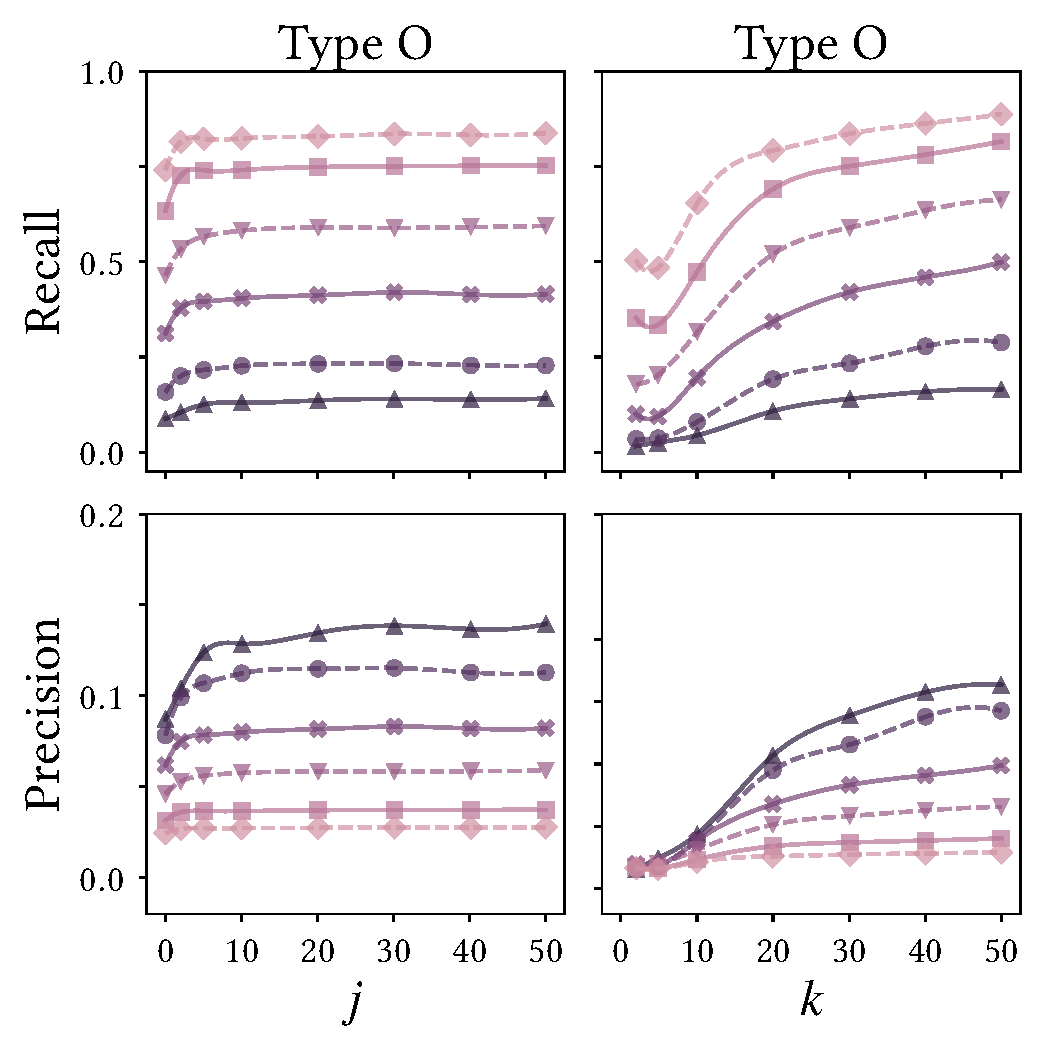
\includegraphics[width=0.49\linewidth]{part4-figures/typeA_wrt_kjp_nyt_1-compressed.pdf}
	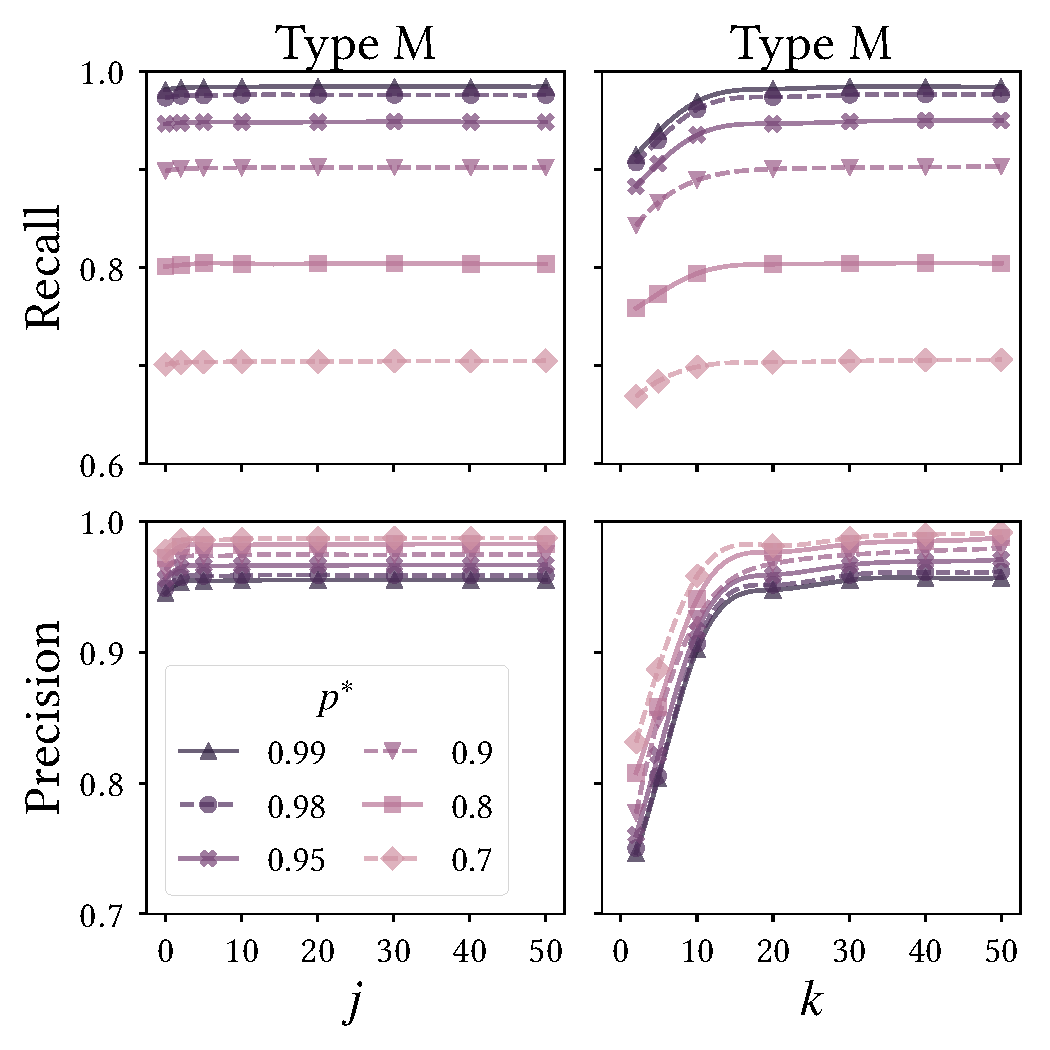
\includegraphics[width=0.49\linewidth]{part4-figures/typeB_wrt_kjp_nyt_1-compressed.pdf}
	\caption{Type O/M -- $k,j,p^*$ sensitivity, NYT-1.}
	\label{fig:typeAB_wrt_kjp}
\end{figure} 

\begin{figure}[ht]
	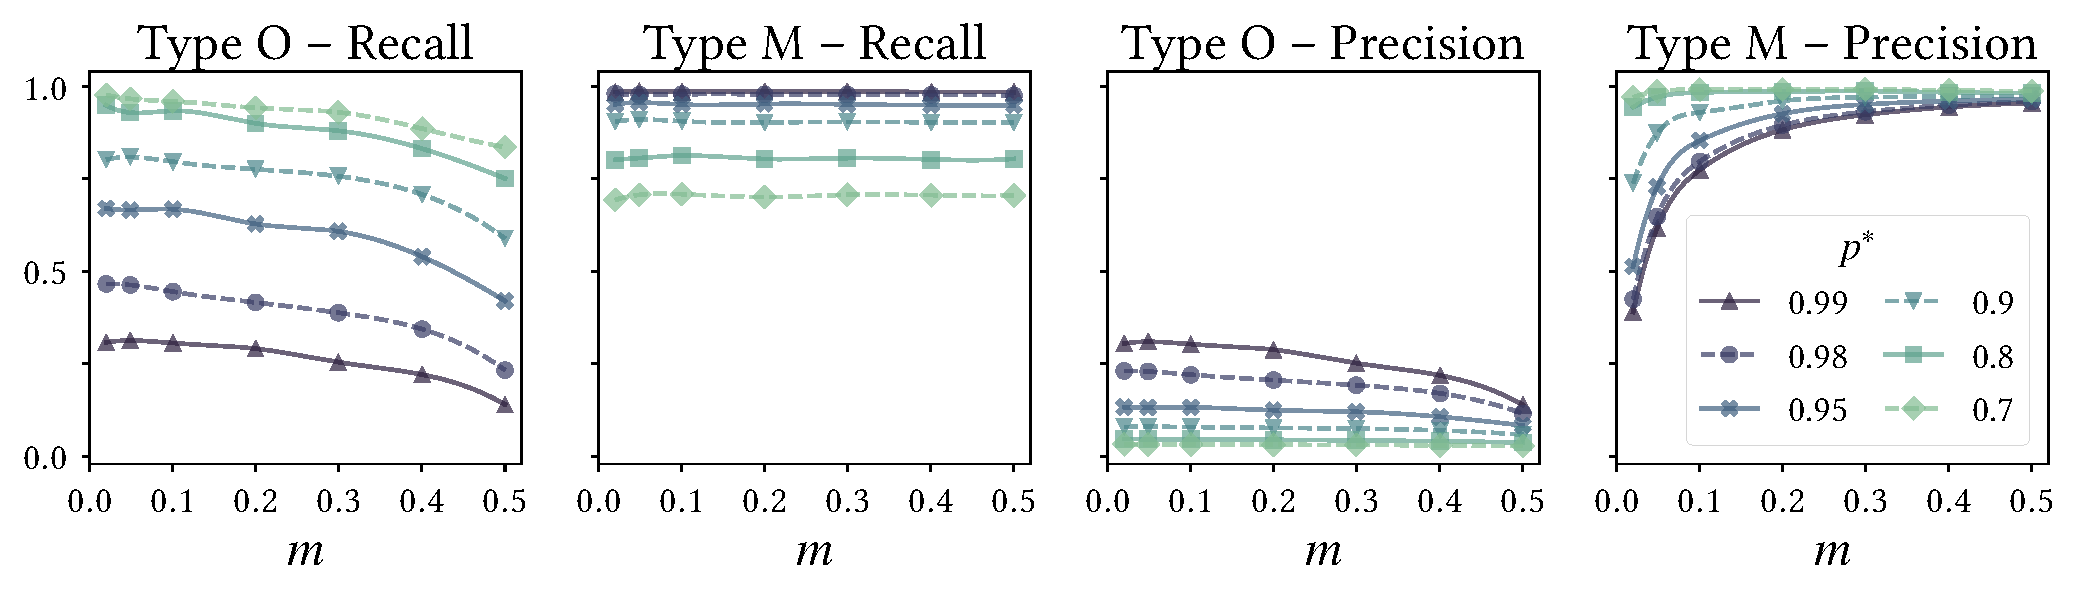
\includegraphics[width=\linewidth]{part4-figures/typeAB_wrt_pc-2-compressed.pdf}
	\caption{Type O/M -- $p^*,m$ sensitivity, NYT-1.}
	\label{fig:typeAB_wrt_pc}
\end{figure}

\subsection{Performance Comparison}

\subsubsection{Type~O}
Table \ref{result:nyt_typeA} and Table \ref{result:arxiv_typeA} list the results of our comparison against the NYT and ARXIV benchmark. First, the results of every approach are generally better against the NYT benchmark. The ARXIV benchmark is much more challenging because the corpus is composed of abstracts from computer science sub-fields, with much semantic overlap.

Then, we see from both tables that \gls{kj-NN} outperforms every competitor w.r.t.\ Type~O outlier detection. The performance in terms of recall becomes lower for smaller data sets (e.g., NYT-20 and NYT-10). For small data sets,  \gls{CVDD} and our \gls{ANCS}/\gls{k-ANCS} baselines appear competitive.  

Finally, we see that our approach handles particularly well multi-modal settings, i.e., with multiple inlier/outlier classes. 
By design, our approach cannot handle only one inlier class (e.g., ARXIV-15) --- this does not fit our scenario. When there only is a single outlier class, \gls{LOF} performs best (see ARXIV-51).
%EF: We could emphasize that LOF is sensitive to parameters. 

\begin{table} %EF: Note: Our approach actually has an unfair handicap, because the labels are noisy (but the other are fully unsupervised). To keep in mind if I ever compare CVDD
\sisetup{detect-weight,mode=text}
\renewrobustcmd{\bfseries}{\fontseries{b}\selectfont}
\renewrobustcmd{\boldmath}{}
    \centering
    \caption{Comparison w.r.t.\ our Competitors (Type O, NYT).}
    \label{result:nyt_typeA}
    \addtolength{\tabcolsep}{-2pt}
    \centering
    \footnotesize
\renewcommand{\arraystretch}{0.68}
    \begin{tabularx}{\columnwidth}{@{}XXXXXXX@{}}
\toprule
Benchmark   & Approach & \gls{AUC} & \gls{AP} & R1\% & R2\% & R5\% \\ \midrule
NYT-1   & \gls{LOF}      & 66.45 &	1.62 &	3.00 &	3.00 &	9.00 \\
        & \gls{RS-Hash}  & 46.62   & 0.87   & 0.00        & 1.00        & 1.00  \\
        & \gls{ANCS}      & 66.63   & 2.57   & 6.00        & 10.00       & 21.00 \\
        & \gls{k-ANCS}    & 83.89  &	3.65 &	3.00 &	7.00 &	19.00 	 \\
        & \gls{TONMF}    & 58.66 	& 7.30 	 & 0.00 	       & 2.00 	     & 9.00 \\
        & \gls{VMF-Q}    & 76.34   & 2.21   &  2.00          & 3.00           & 11.00  \\
        & \gls{CVDD}     & 78.47 &	7.75&	11.7 & 18.09	 & 22.34  \\
        & \gls{kj-NN} &\bfseries 92.51 &\bfseries	17.57 &\bfseries	25.00 &\bfseries	39.20 &\bfseries	61.40 \\ \midrule


NYT-2   & \gls{LOF}      & 60.66  &	2.45 &	2.00 &	2.50 &	6.00   \\   
        & \gls{RS-Hash}  & 48.05   & 1.87   & 0.50    & 1.00  &  5.50   \\
        & \gls{ANCS}      & 67.59   & 5.19   & 8.00    & 12.00 & 18.00   \\
        & \gls{k-ANCS}    & 82.51  &	5.94 &	3.00 &	5.50 &	14.50    \\    
        & \gls{TONMF}    & 54.61 	 & 1.78   & 2.50 	& 3.00 	& 9.00 	 \\           
        & \gls{VMF-Q}    & 83.67   & 6.87   & 4.00    & 11.00 & 20.00   \\
        & \gls{CVDD}     & 73.10 &	10.00 &	11.58&	14.74 &	22.11  \\
        & \gls{kj-NN}    & \bfseries 94.51 &\bfseries	42.64 &\bfseries	30.40 &\bfseries	44.50 &\bfseries	64.50   \\    \midrule

NYT-5    & \gls{LOF}     & 52.28 & 5.44  & 1.80  & 3.40  & 7.00  \\
         & \gls{RS-Hash} & 48.76 & 4.58  & 0.80  & 1.40  & 2.80  \\
         & \gls{ANCS}     & 67.67 & 11.13 & 6.60  & 9.80  & 19.20 \\
         & \gls{k-ANCS}   & 75.56 & 10.45 & 3.40  & 6.40  & 11.40 \\
         & \gls{TONMF}   & 52.95 &	1.50 &	1.40  &	2.40 &	6.40      \\
         & \gls{VMF-Q}   & 77.11 & 12.92 & 4.60  & 7.40  & 15.60 \\
         & \gls{CVDD}     & 72.81	& 18.69	 & 9.04	 &13.05	 & 21.49  \\
         & \gls{kj-NN}   &\bfseries 97.04 &\bfseries	71.69 &\bfseries	19.12 &\bfseries	36.96 &\bfseries	68.28 \\ \midrule

NYT-50   & \gls{LOF}     & 60.91 &	1.77 &	2.00 &	6.00 &	12.00 	 \\
         & \gls{RS-Hash} & 46.14 & 0.90  & 0.00  & 0.00  & 2.00  \\
         & \gls{ANCS}     & 63.94 & 4.35  & 14.00 & 16.00 & 20.00 \\
         & \gls{k-ANCS}   & 81.08 &	4.43 &	12.00 &	14.00 &	20.00 	 \\
         & \gls{TONMF}   & 61.42 & \bfseries 31.01 &	0.90 &	0.90 &	4.90  \\
         & \gls{VMF-Q}   & 85.76 & 4.00  & 6.00  & 8.00  & 22.00 \\
         & \gls{CVDD}     &76.29	& 15.89	 & 21.62 &	27.03 &	29.73 \\
         & \gls{kj-NN}   &\bfseries 93.33 &	27.76 &\bfseries	37.20 &\bfseries 	46.80 &\bfseries 	62.80 	 \\ \midrule

NYT-20   & \gls{LOF}     & 74.76 &	4.12 &	5.00 &	5.00 &	15.00 	 \\
         & \gls{RS-Hash} & 42.91 & 0.89  & 0.00  & 0.00  & 0.00  \\
         & \gls{ANCS}     & 78.52 & 5.60  & 10.00 & 15.00 & \bfseries40.00 \\
         & \gls{k-ANCS}   & 88.56  &	6.59 &	15.00  & 20.00 &	30.00 \\
         & \gls{TONMF}   & 64.94 & 6.35  & 0.00 	 & 0.00 	 & 15.00  \\
         & \gls{VMF-Q}   & 83.98 & 4.59  & 5.00  & 10.00 & 20.00 \\
         & \gls{CVDD}     & 88.83 & \bfseries 24.00 & \bfseries25.00	& \bfseries25.00 &	25.00  \\
         & \gls{kj-NN}   &\bfseries 91.42 &	6.57 &	3.00 &	11.00 &	38.00 \\ \midrule

NYT-10   & \gls{LOF}     & 77.93 & 	2.77 &	0.00 &	0.00 &	20.00 \\
         & \gls{RS-Hash} & 56.94 & 1.76  & 0.00  & 0.00  & 10.00 \\
         & \gls{ANCS}     & 83.89 & 13.65 & 30.00 & 40.00 & 40.00 \\
         & \gls{k-ANCS}   & 91.37 &	10.93 & 30.00 &	30.00 &	30.00 	 \\
         & \gls{TONMF}   & 71.13 & 29.92 &	0.00 &	0.00 &	0.00 \\
         & \gls{VMF-Q}   & 63.39 & 2.55  & 0.00  & 10.00 & 20.00 \\
         & \gls{CVDD}     & 85.13	& \bfseries44.99	& \bfseries42.86 &	\bfseries42.86	 & \bfseries42.86 \\
         & \gls{kj-NN}   & \bfseries 91.52 &	8.45 &	10.00 &	16.00 &	38.00 \\ \bottomrule
\end{tabularx}
\end{table}

\begin{table}
\sisetup{detect-weight,mode=text}
\renewrobustcmd{\bfseries}{\fontseries{b}\selectfont}
\renewrobustcmd{\boldmath}{}
    \centering
    \caption{Comparison w.r.t.\ our Competitors (Type O, ARXIV).}
    \label{result:arxiv_typeA}
    \addtolength{\tabcolsep}{-3pt}
    \centering
    \footnotesize
\renewcommand{\arraystretch}{0.35}
    \begin{tabularx}{\columnwidth}{@{}XXXXXXX@{}}
\toprule
Benchmark   & Approach & \gls{AUC} & \gls{AP} & R1\% & R2\% & R5\% \\ \midrule

ARXIV-15 & \gls{LOF}     & 63.44 &	1.78 &	0.00 &	5.13 &	7.69 	 \\
         & \gls{RS-Hash} & 54.22 & 1.17  & 2.56  & 2.56  & 2.56  \\
         & \gls{ANCS}     & 47.46 & 0.96  & 0.00  & 0.00  & 5.13  \\
         & \gls{k-ANCS}   & 67.14  &	1.98 &	0.00 &	7.69 &	10.26 \\
         & \gls{TONMF}   & 57.65 	& \bfseries7.32  &	0.00  &	7.69 &	15.38 	     \\
         & \gls{VMF-Q}   & \bfseries71.71 & 2.69  & \bfseries 5.13  & \bfseries10.26 & 15.38 \\
         & \gls{CVDD}     & 69.85	& 2.27 &	0.00 &	5.13 &	\bfseries17.95  \\
         & \gls{kj-NN}   & 54.21 & 1.17  & 0.00  & 0.00  & 0.00  \\ \midrule

ARXIV-25 & \gls{LOF}     & 68.41 & 2.17  & 4.35  & 6.52  & 13.04 \\
         & \gls{RS-Hash} & 44.21 & 0.91  & 0.00  & 0.00  & 4.35  \\
         & \gls{ANCS}     & 47.88 & 1.09  & 2.17  & 4.35  & 6.52  \\
         & \gls{k-ANCS}   & 67.87 & 2.00  & 2.17  & 4.35  & 10.87 \\
         & \gls{TONMF}   & 60.03 & \bfseries6.37 &	0.00   & 4.35 & 13.04      \\
         & \gls{VMF-Q}   & 71.71 & 2.69  & 5.13  & 10.26 & 15.38 \\
         & \gls{CVDD}     & \bfseries 74.55 & 2.19	& 2.17	& 4.35	& 8.70  \\
         & \gls{kj-NN}   & 70.64 &	5.10 &\bfseries	10.44 &\bfseries	16.52 &\bfseries	27.82 	 \\ \midrule

ARXIV-35 & \gls{LOF}     & 71.00 &	2.16 &	0.00 &	3.23 &	11.29 \\
         & \gls{RS-Hash} & 47.77 & 0.96  & 1.61  & 1.61  & 4.84  \\
         & \gls{ANCS}     & 52.94 & 1.07  & 0.00  & 0.00  & 3.23  \\
         & \gls{k-ANCS}   & 73.43 &	2.36 &	1.61 &	4.84 &	16.13 \\
         & \gls{TONMF}   & 56.90 & 1.16  & 1.61  & 3.22  & 6.45      \\
         & \gls{VMF-Q}   & 60.97 & 1.28  & 0.00  & 0.00  & 1.61  \\
         & \gls{CVDD}     & 53.89 &	1.06 &	0.00 &	0.00 &	1.61 \\
         & \gls{kj-NN}   & \bfseries73.58 &\bfseries	3.27 &\bfseries	6.45 &\bfseries	10.97 &\bfseries	20.97 	 \\ \midrule

ARXIV-45 & \gls{LOF}     & 62.99 	& 2.43 	& 2.02 	& 2.02 & 5.05  \\
         & \gls{RS-Hash} & 49.18 & 0.99  & 0.00  & 0.00  & 6.06  \\
         & \gls{ANCS}     & 51.50 & 1.32  & 1.01  & 1.01  & 2.02  \\
         & \gls{k-ANCS}   & 70.11 & 2.23  & 1.01  & 3.03  & 17.17 \\
         & \gls{TONMF}   & 57.49   & \bfseries17.23 & 0.00 	 & 0.00  & 2.02 \\
         & \gls{VMF-Q}   & 66.59 & 2.20  & 3.03  & 7.07  & 15.15 \\
         & \gls{CVDD}     & \bfseries71.32 &	2.10 &	2.02 &	4.04 &	11.11  \\
         & \gls{kj-NN}   & 69.94 &	3.28 &\bfseries	6.46&\bfseries 	9.09 &\bfseries	18.99 \\ \midrule

ARXIV-55 & \gls{LOF}     & 59.47 	& 1.47 	& 3.23 & 	3.23 &	11.29 \\
         & \gls{RS-Hash} & 49.00 & 0.94  & 0.81  & 0.81  & 3.23  \\
         & \gls{ANCS}     & 51.69 & 1.80  & 1.61  & 3.23  & 6.45  \\
         & \gls{k-ANCS}   & 67.59 &	2.25 &	3.23 &	6.45 &	14.52 	 \\
         & \gls{TONMF}   & 56.86 & 0.92  & 1.61  & 3.23  & 9.68    \\
         & \gls{VMF-Q}   & 72.99 & 2.65  & 4.84  & 8.06  & 16.94 \\
         & \gls{CVDD}     & 60.92	& 1.63	& 1.61	& 4.84	& 11.29  \\
         & \gls{kj-NN}   & \bfseries76.74 & \bfseries	3.22 & \bfseries	5.49 & \bfseries	9.84 & \bfseries	20.48 \\ \midrule

ARXIV-54 & \gls{LOF}     & 61.92 & 1.33  & 0.00  & 2.42  & 6.45  \\
         & \gls{RS-Hash} & 47.95 & 0.92  & 0.00  & 0.81  & 2.42  \\
         & \gls{ANCS}     & 50.46 & 1.01  & 0.81  & 0.81  & 3.23  \\
         & \gls{k-ANCS}   & 68.93 &	1.83 &	0.00 &	1.61 &	8.87 	  \\
         & \gls{TONMF}   & 59.46 & \bfseries5.94  & 0.00  & 0.00  & 6.45     \\
         & \gls{VMF-Q}   & 61.81 & 1.33  & 0.81  & 1.61  & 6.45  \\
         & \gls{CVDD}     & 60.30	& 1.62	& 1.61	 &5.65	& 10.48  \\
         & \gls{kj-NN}   & \bfseries76.65 &	3.85 & \bfseries	5.81 & \bfseries	10.00 & \bfseries	21.61 \\ \midrule

ARXIV-53 & \gls{LOF}     & 57.37 & 1.33  & 2.42  & 3.23  & 9.68  \\
         & \gls{RS-Hash} & 42.32 & 0.79  & 0.00  & 0.00  & 0.00  \\
         & \gls{ANCS}     & 47.55 & 0.93  & 0.81  & 1.61  & 3.23  \\
         & \gls{k-ANCS}   & 63.56 &	1.54 &	2.42 &	4.03 &	9.68  \\
         & \gls{TONMF}   & 56.12 & 4.26  & 0.00  & 1.61  & 8.06      \\
         & \gls{VMF-Q}   & 77.29 & 3.16  & 3.23  & 8.06  & 25.00 \\
         & \gls{CVDD}     & 69.28	& 1.98 &	2.42 &	4.03 &	12.90  \\
         & \gls{kj-NN}   & \bfseries79.16 & \bfseries	5.10 & \bfseries	7.74 & \bfseries	15.65 & \bfseries	32.42 	 \\ \midrule

ARXIV-52 & \gls{LOF}     & 55.58 & 1.09  & 0.81  & 0.81  & 4.84  \\
         & \gls{RS-Hash} & 52.52 & 1.08  & 0.00  & 1.61  & 5.65  \\
         & \gls{ANCS}     & 45.02 & 0.84  & 0.00  & 0.00  & 0.81  \\
         & \gls{k-ANCS}   & 66.26 &	1.61 &	0.81 &	3.23 &	8.87 \\
         & \gls{TONMF}   & 54.04  & 	2.70 &	1.61 	& 3.23  &	8.06   \\
         & \gls{VMF-Q}   & 67.57 & 2.06  & 2.42  & 7.26  & 13.71 \\
         & \gls{CVDD}     & 55.64	& 1.39	& 1.61 &	4.84 &	11.29  \\
         & \gls{kj-NN}   & \bfseries 78.10 & \bfseries	3.07 & \bfseries	3.87 & \bfseries	7.90 & \bfseries	19.35 	\\ \midrule

ARXIV-51 & \gls{LOF}     & \bfseries82.57 &\bfseries	4.50 	&\bfseries7.26  &\bfseries	14.52 &\bfseries 	25.81 \\
         & \gls{RS-Hash} & 51.22 & 1.10  & 1.61  & 4.03  & 6.45  \\
         & \gls{ANCS}     & 65.91 & 2.36  & 5.65  & 10.48 & 15.32 \\
         & \gls{k-ANCS}   & 54.19 &	1.68 &	4.03 &	7.26 &	11.29 	 \\
         & \gls{TONMF}   & 55.23  &	1.01 &	1.61 &	1.61 &	7.26   \\
         & \gls{VMF-Q}   & 62.54 & 1.54  & 1.61  & 4.84  & 8.87  \\
         & \gls{CVDD}     & 66.93	 & 2.54	 & 4.84	& 8.87 &	23.39  \\
         & \gls{kj-NN}   & 65.24 	& 2.19 &	4.68 &	7.90  & 14.36 \\ \bottomrule
\end{tabularx}
\end{table}

\subsubsection{Type M} Our approach also outperforms its competitors w.r.t.\ Type~M outliers. See Tables \ref{result:nyt_typeB} and \ref{table:arxiv_typeB}. 
\gls{RCNN} and \gls{VD-CNN} have high precision, but much lower recall. Neural networks tend to fit the data very well, including Type~M outliers. The performance decreases dramatically with smaller data sets. \gls{VD-CNN} occasionally ranks high in terms of F1-score. However, those approaches do not rank outliers, so the recall at a certain percentage (e.g., R10, R20) is equivalent to that from a list of detected outliers in random order.

\begin{table}
\sisetup{detect-weight,mode=text}
\renewrobustcmd{\bfseries}{\fontseries{b}\selectfont}
\renewrobustcmd{\boldmath}{}
    \centering
    \caption{Comparison w.r.t.\ our Competitors (Type M, NYT).}
    \label{result:nyt_typeB}
\addtolength{\tabcolsep}{-3pt}
    \centering
    \footnotesize
\renewcommand{\arraystretch}{0.45}
    \begin{tabularx}{\columnwidth}{@{}XXXXXXX@{}}
\toprule
Benchmark & Approach  & P     & R     & F1      & R10\%  & R20\%  \\ \midrule
NYT-1    & \gls{W-CNN}     & 54.38   & 86.04   & 66.64     & 27.28 & 53.51 \\
         & \gls{VD-CNN}    & 90.71   & 69.22   & 78.52     & 15.04 & 30.18 \\
          & \gls{AT-RNN}   & 67.12   & 51.88   & 58.52    & 32.92 & 51.34 \\
          & \gls{RCNN}      &\bfseries 96.02 & 9.65    & 17.54    & 9.55  & 9.55  \\
          & \gls{kj-NN}     & 95.93 &\bfseries	90.02 &\bfseries	92.88 &\bfseries	50.19 &\bfseries	90.02	 \\ \midrule
          
NYT-2    & \gls{W-CNN}     & 54.16   & 88.02 & 67.06 & 27.30 & 54.56 \\
         & \gls{VD-CNN}    & 88.99   & 69.69 & 78.17  & 14.71 & 29.61 \\
         &\gls{AT-RNN}   & 80.36   & 49.03 & 60.90 & 40.29 & 48.14 \\
         & \gls{RCNN}      & 89.60   & 5.59  & 10.52  & 5.49  & 5.49  \\
         & \gls{kj-NN}     &\bfseries 94.63 &\bfseries	91.15 &\bfseries	92.86 &\bfseries	50.74 &\bfseries	91.15 \\ \midrule
          
NYT-5   & \gls{W-CNN}     & 51.12 & 89.07 & 64.96 & 25.14 & 50.38 \\    
        & \gls{VD-CNN}    & 58.21 & 82.39 & 68.22 & 8.98  & 18.46 \\
        & \gls{AT-RNN}   & 61.71 & 70.49 & 65.81 & 31.38 & 61.62 \\
        & \gls{RCNN}      & 90.82 & 44.93 & 60.12 & 42.86 & 42.86 \\
        & \gls{kj-NN}     & \bfseries 92.43 &\bfseries	93.44 &\bfseries	92.93 &\bfseries	52.27 &\bfseries	93.44 \\ \midrule
          
NYT-50   & \gls{AT-RNN}   & 47.38 & 87.61 & 61.50 & 22.28 & 47.62 \\
          & \gls{RCNN}      & \bfseries98.58 & 55.44 & 70.97 & 49.31 & 54.95 \\
          & \gls{VD-CNN}    & 89.75 & 69.22 & 78.16 & 14.83 & 29.92 \\
          & \gls{W-CNN}     & 57.46 & 87.31 & 69.31 & 27.23 & 56.93 \\
          & \gls{kj-NN}     & 95.78 &\bfseries	90.36 &\bfseries	92.99 &\bfseries	50.22 &\bfseries	90.36 \\ \midrule
          
NYT-20   & \gls{W-CNN}     & 39.34 & \bfseries91.56 & 55.03 & 20.54 & 40.59 \\
         & \gls{VD-CNN}    & 93.50 & 81.80 & 87.26 & 15.20 & 30.81 \\
         & \gls{AT-RNN}   & 50.44 & 85.11 & 63.34 & 25.25 & 52.23 \\
         & \gls{RCNN}      & 39.63 & \bfseries91.56 & 55.32 & 20.54 & 40.59 \\
         & \gls{kj-NN}     &\bfseries 93.80 &	90.64 &\bfseries	92.19 &\bfseries	50.52 &\bfseries	90.64 \\  \midrule
          
NYT-10   & \gls{W-CNN}     & 36.12 & 88.94 & 51.38 & 16.83 & 35.15 \\
         & \gls{VD-CNN}    & 86.20 & 69.40 & 76.89  & 14.10 & 27.26 \\
         & \gls{AT-RNN}   & 36.12 & 88.94 & 51.38 & 16.83 & 35.15 \\
         & \gls{RCNN}      & 36.12 & 88.94 & 51.38 & 16.83 & 35.15 \\
         & \gls{kj-NN}     & \bfseries 88.57 &\bfseries	90.77 &\bfseries	89.65 &\bfseries	50.50 &\bfseries	89.97 \\ \bottomrule

\end{tabularx}
\end{table}

\begin{table}
\sisetup{detect-weight,mode=text}
\renewrobustcmd{\bfseries}{\fontseries{b}\selectfont}
\renewrobustcmd{\boldmath}{}
    \centering
    \caption{Comparison w.r.t.\ our Competitors (Type M, ARXIV).}
    \label{table:arxiv_typeB}
    \addtolength{\tabcolsep}{-2pt}
    \centering
    \footnotesize
\renewcommand{\arraystretch}{0.77}
    \begin{tabularx}{\columnwidth}{XXXXXXX}
\toprule
Benchmark & Approach  & P     & R     & F1      & R10\%  & R20\%  \\ \midrule
ARXIV-25    & \gls{W-CNN}     & 95.33 &	82.51 &	88.46 &	47.77 &	82.15 	 \\
         & \gls{VD-CNN}    & 72.97 &	59.71 &	65.68 &	15.52 &	31.60 	 \\
          & \gls{AT-RNN}   & 65.90 &	72.24 &	68.92 &	32.97 &	65.94 	 \\
          & \gls{RCNN}      & 96.75 &	26.01 &	41.00 &	25.90 &	25.90 \\
          & \gls{kj-NN}     & \bfseries96.09 &	\bfseries88.85 &	\bfseries92.33 &	\bfseries49.22 &	\bfseries88.85 \\ \midrule
ARXIV-35    & \gls{W-CNN}     & 54.97 &	84.40 &	66.58 &	27.45 &	54.49 	 \\
         & \gls{VD-CNN}    & 66.06 &	80.08 &	72.40 &	11.73 &	23.01 	 \\
          & \gls{AT-RNN}   & \bfseries 84.37 &	38.59 &	52.96 &	38.12 &	38.12 	 \\
          & \gls{RCNN}      & 80.21 &	25.02 &	38.14 &	24.72 &	24.72 	 \\
          & \gls{kj-NN}     & 80.04 &	\bfseries86.98  & \bfseries83.36 & \bfseries48.25 & \bfseries83.40 \\ \midrule
ARXIV-45    & \gls{W-CNN}     & 51.47 &	81.26 &	63.02 &	24.80 &	49.40 	 \\
         & \gls{VD-CNN}    & 73.68 &	72.24 &	72.95 &	10.48 &	21.00 \\
          & \gls{AT-RNN}   & \bfseries74.20 &	49.97 &	59.72 &	37.70 &	49.60 \\
          & \gls{RCNN}      & 65.49 &	26.10 &	37.32 &	25.90 &	25.90 \\
          & \gls{kj-NN}     & 70.29 &	\bfseries86.87 &	\bfseries77.70  &	\bfseries45.78  & \bfseries 76.89 \\ \midrule
ARXIV-55    & \gls{W-CNN}     & 53.62 &	87.71 &	66.55 &	27.79 &	53.66 \\
         & \gls{VD-CNN}    & \bfseries92.65 & \bfseries91.97 &	\bfseries92.31 &	12.01 &	24.08 \\
          & \gls{AT-RNN}   & 86.50 &	54.56 &	66.91 &	43.07 &	54.06 	 \\
          & \gls{RCNN}      & 83.80 &	33.87 &	48.24 &	33.56 &	33.56 	 \\
          & \gls{kj-NN}     & 70.70 &	88.23 &	78.50 &	\bfseries46.77 & \bfseries78.67 \\ \midrule
ARXIV-54    & \gls{W-CNN}     & 58.07 &	87.94 &	69.95 &	28.03 &	57.40 \\
         & \gls{VD-CNN}    & \bfseries87.22 & 	85.12 &\bfseries	86.16 &	11.38 &	22.71  \\
          & \gls{AT-RNN}   & 69.81 &	56.33 &	62.35 &	34.79 &	55.77 \\
          & \gls{RCNN}      & 58.10 &	41.09 &	48.14 &	28.98 &	40.68 \\
          & \gls{kj-NN}     & 70.38 &	\bfseries88.05 &	78.23 &	\bfseries46.83 &	\bfseries77.78 \\ \midrule
ARXIV-53    & \gls{W-CNN}     & 47.12 &	85.91 &	60.86 &	24.56 &	47.97 \\
         & \gls{VD-CNN}    & \bfseries82.78 &	82.64 &\bfseries	82.71 &	10.95 &	21.62 	 \\
          & \gls{AT-RNN}   & 58.65 &	60.31 &	59.47 &	29.22 &	58.48 \\
          & \gls{RCNN}      & 63.25 &	22.58 &	33.28 &	22.33 &	22.33 	 \\
          & \gls{kj-NN}     & 70.77 &	\bfseries88.46 &	78.63 &	\bfseries46.69 &	\bfseries78.24 \\ \midrule
ARXIV-52    & \gls{W-CNN}     & 49.10 &	84.35& 	62.07 &	24.84 &	49.12 	\\
         & \gls{VD-CNN}    & \bfseries86.92 &	\bfseries91.59 	& \bfseries89.19 &	11.49 &	22.77 \\
          & \gls{AT-RNN}   & 78.94 & 61.65 &	69.23 &	39.41 &	60.87 	 \\
          & \gls{RCNN}      & 45.24 &	27.02 &	33.83 &	22.53 &	26.67 	 \\
          & \gls{kj-NN}     & 71.08 &	88.43 &	78.81 &	\bfseries47.28 &	\bfseries78.79 \\ \midrule
ARXIV-51    & \gls{W-CNN}     & 56.00 &	\bfseries86.47 &	67.98 &	28.14 &	56.49 	 \\
         & \gls{VD-CNN}    &78.89  &	82.56 &	\bfseries80.68 &	10.24 &	20.42 	 	 	 \\
          & \gls{AT-RNN}   & 76.27 &	59.04 &	66.56 &	38.57 &	58.36 \\
          & \gls{RCNN}      & \bfseries79.67 &	25.09 &	38.16 &	24.80 &	24.80 \\ 
          & \gls{kj-NN}     & 70.91 &	88.63 &	78.79 &	\bfseries46.25 &	\bfseries78.18 \\ \bottomrule
\end{tabularx}
\end{table}

\subsubsection{Ablation Analysis}
\label{ablationanalysis}

We verify each of our design choices by comparing against the following ablations:  
\begin{itemize}[noitemsep]
    \item \textbf{A1: No self-supervision}; we set $j=0$, i.e., our approach boils down to a k-NN classifier as in Equation \ref{eq:traditional-knn}. \item \textbf{A2: No entropy}; we do not estimate the entropy of the prediction, i.e., objects can be in both outlier lists $\mathbb{O}$ and $\mathbb{M}$.
    \item \textbf{A3: No neighbourhood}; the predictions only base on the relevance of document $\gls{d}$, and not on the relevance of its neighbours, i.e., we set $\mathcal{K}(\gls{d}) = \{\gls{d}\}$. 
    \item \textbf{A4: Unweighted \gls{kj-NN}}; we do not weigh the score by the inter-document and document-phrase similarities, as explained in Section \ref{sec: Implementation}. Each neighbouring document and phrase have the same impact on the decision. 
\end{itemize}
From Table \ref{tab:ablation_nyt} and  \ref{tab:ablation_arxiv}, we can see that \gls{kj-NN} consistently outperforms every ablation on average. A2 leads to higher Type~M recall, and often high Type~O \acrshort{AUC}, but much lower Type~M precision. 
A1 and A3 yield worse results for both outlier types. A4 values are consistently below, but only by a few hundredth. 
The overall average ranks are as follows: 
\begin{itemize}[noitemsep]
    \item \textbf{\gls{kj-NN}:} 1.67, \textbf{A2:} 2.50, \textbf{A4:} 2.69, \textbf{A1:} 3.30, \textbf{A3:} 4.29
\end{itemize}
Thus, we can see that taking the neighbourhood into account improves the performance of our approach the most, followed by self-supervision. Measuring decision uncertainty and weighting by similarity, as in Equation \ref{eq:weightkjnn}, improves the performance further. 

\begin{table}[ht]
\caption{Ablation Analysis (NYT).}
\label{tab:ablation_nyt}
\sisetup{detect-weight,mode=text}
\renewrobustcmd{\bfseries}{\fontseries{b}\selectfont}
\renewrobustcmd{\boldmath}{}
\addtolength{\tabcolsep}{-2pt}
    \centering
    \footnotesize
\renewcommand{\arraystretch}{0.67}
\begin{tabularx}{\columnwidth}{XXXXXXX|c}
                  &       &  \multicolumn{2}{c|}{Type A }  &    \multicolumn{3}{c}{Type B}   &  \xrowht{8pt}  \\ \cline{3-4}\cline{5-7}
Benchmark          &    Ablation   & \gls{AUC}    & \gls{AP}    & P      & R           & F1    & Rank\xrowht{8pt}  \\  \toprule 
NYT-1    & A1    & 89.57  & 16.65 & 94.56  & 90.04       & 92.25 & 3.6  \\
          & A2    & \bfseries92.51  & \bfseries17.57 & 86.43  & \bfseries99.07       & 92.32 & 2.2  \\
          & A3    & 90.56  & 8.45  & 91.85  & 89.28       & 90.54 & 4.6  \\
          & A4    & 92.48  & 17.07 & 95.88  & 90.00       & 92.85 & 2.8  \\
          & \gls{kj-NN} & \bfseries92.51  & \bfseries17.57 & \bfseries95.93  & 90.02       & \bfseries92.88 & \bfseries1.4  \\ \midrule
NYT-2    & A1    & 93.29  & \bfseries43.23 & 93.61  & 91.23       & 92.40 & 2.6  \\
          & A2    & \bfseries94.51  & 42.64 & 83.15  & \bfseries99.32       & 90.52 & 2.6  \\
          & A3    & 91.23  & 18.62 & 90.22  & 89.89       & 90.05 & 4.8  \\
          & A4    & 94.50  & 42.12 & 94.55  & 91.07       & 92.78 & 2.8  \\
          & \gls{kj-NN} &\bfseries94.51  & 42.64 & \bfseries94.63  & 91.15       & \bfseries92.86 & \bfseries1.6  \\ \midrule
NYT-5    & A1    & 96.61  & \bfseries72.33 & 92.12  & 93.55       & 92.83 & 2.6  \\
          & A2    & \bfseries97.04  & 71.69 & 75.92  & \bfseries99.18       & 86.01 & 2.8  \\
          & A3    & 92.33  & 41.43 & 86.12  & 91.97       & 88.95 & 4.6  \\
          & A4    & \bfseries97.04  & 71.63 & 92.23  & 93.45       & 92.84 & 2.4  \\
          & \gls{kj-NN} & \bfseries97.04  & 71.69 & \bfseries92.43  & 93.44       & \bfseries92.93 & \bfseries1.8  \\ \midrule
NYT-50   & A1    & 91.20  & 27.29 & 94.20  & 90.36       & 92.24 & 3.2  \\
          & A2    & \bfseries93.33  & \bfseries27.76 & 85.40  & \bfseries99.34       & 91.84 & 2.4  \\
          & A3    & 90.78  & 13.34 & 92.68  & 89.11       & 90.86 & 4.8  \\
          & A4    & 93.30  & 27.44 & 95.64  & 90.34       & 92.91 & 2.8  \\
          & \gls{kj-NN} & \bfseries93.33  & \bfseries27.76 & \bfseries95.78  & 90.36       & \bfseries92.99 & \bfseries1.2  \\  \midrule
NYT-20   & A1    & 89.01  & 5.94  & 93.10  & 90.29       & 91.67 & 4.0    \\
          & A2    & \bfseries91.42  & 6.57  & 83.56  & \bfseries98.90       & 90.58 & 2.6  \\
          & A3    & 89.93  & \bfseries9.45  & 91.19  & 87.44       & 89.27 & 3.8  \\
          & A4    & \bfseries91.42  & 6.51  & 93.60  & 90.49       & 92.02 & 2.2    \\
          & \gls{kj-NN} & \bfseries91.42  & 6.57  & \bfseries93.80  & 90.64       & \bfseries92.19 & \bfseries1.4  \\ \midrule
NYT-10   & A1    & 91.25  & 8.05  & 88.18  & 90.47       & 89.31 & 3.6  \\
          & A2    & \bfseries91.52  & 8.45  & 80.98  & \bfseries98.50       & 88.88 & 2.6  \\
          & A3    & 89.65  & 14.06 & 87.30  & 85.17       & 86.20 & 4.6  \\
          & A4    & 91.23  & \bfseries8.49  & 88.19  & 90.57       & 89.36 & 2.4  \\
          & \gls{kj-NN} & \bfseries91.52  & 8.45  & \bfseries88.57  & 90.77       & \bfseries89.65 & \bfseries1.4  \\ 
 \bottomrule
\end{tabularx}
\end{table} 

\begin{table}
	\caption{Ablation Analysis (ARXIV).}
	\label{tab:ablation_arxiv}
	\sisetup{detect-weight,mode=text}
	\renewrobustcmd{\bfseries}{\fontseries{b}\selectfont}
	\renewrobustcmd{\boldmath}{}
	\addtolength{\tabcolsep}{-2pt}
	\centering
	\footnotesize
	\renewcommand{\arraystretch}{0.55}
	\begin{tabularx}{\columnwidth}{XXXXXXX|c}
		&       &  \multicolumn{2}{c|}{Type A }  &    \multicolumn{3}{c}{Type B}   &  \xrowht{8pt}  \\ \cline{3-4}\cline{5-7}
		Benchmark          &    Ablation   & \gls{AUC}    & \gls{AP}    & P      & R           & F1    & Rank\xrowht{8pt}  \\  \toprule 
		ARXIV-25 & A1    & 67.75  & 3.70  & 95.01  & 88.93       & 91.87 & 4.4  \\
		& A2    & 70.64  & 5.10  & 91.22  & \bfseries98.17       & \bfseries94.56 & 2.2  \\
		& A3    & \bfseries81.23  & \bfseries5.93  & \bfseries97.30  & 88.16       & 92.50 & \bfseries2.0    \\
		& A4    & 70.48  & 5.09  & 96.10  & 88.98       & 92.40 & 3.0    \\
		& \gls{kj-NN} & 70.64  & 5.10  & 96.09  & 88.85       & 92.33 & 3.0    \\  \midrule
		ARXIV-35 & A1    & 71.98  & 3.02  & 80.03  & 87.14       & \bfseries83.43 & 2.8  \\
		& A2    & 73.58  & \bfseries3.27  & 72.75  & \bfseries95.60       & 82.62 & 2.4  \\
		& A3    & \bfseries74.14  & 2.72  & 71.60  & 84.32       & 77.44 & 4.2  \\
		& A4    & 73.54  & \bfseries3.27  & 79.92  & 86.99       & 83.30 & 2.8  \\
		& \gls{kj-NN} & 73.58  & \bfseries3.27  & \bfseries80.04  & 86.98       & 83.36 & \bfseries2.0    \\ \midrule
		ARXIV-45 & A1    & 69.42  & 2.96  & 70.02  & 86.64       & 77.45 & 4.0    \\
		& A2    & 69.94  & \bfseries3.28  & 63.93  & \bfseries95.41       & 76.56 & 2.6  \\
		& A3    & \bfseries71.56  & 3.17  & 65.43  & 84.83       & 73.87 & 3.8  \\
		& A4    & 69.88  & 3.27  & 70.09  & 86.88       & 77.59 & 2.6  \\
		& \gls{kj-NN} & 69.94  & \bfseries3.28  & \bfseries70.29  & 86.87       & \bfseries77.70 & \bfseries1.6  \\ \midrule
		ARXIV-55 & A1    & 75.84  & 3.07  & 70.33  & 88.24       & 78.27 & 3.2  \\
		& A2    & \bfseries76.74  & \bfseries3.22  & 63.78  & \bfseries96.82       & 76.90 & 2.4  \\
		& A3    & 72.31  & 2.24  & 66.06  & 87.02       & 75.10 & 4.8  \\
		& A4    & 76.60  & 3.18  & 70.49  & 88.19       & 78.35 & 2.8  \\
		& \gls{kj-NN} & \bfseries76.74  & \bfseries3.22  & \bfseries70.70  & 88.23       & \bfseries78.50 & \bfseries1.4  \\ \midrule
		ARXIV-54 & A1    & 75.54  & 3.63  & 70.19  & 87.95       & 78.07 & 3.6  \\
		& A2    & \bfseries76.65  & \bfseries3.85  & 63.38  & \bfseries96.94       & 76.65 & 2.4  \\
		& A3    & 76.33  & 3.40  & 66.09  & 86.68       & 75.00 & 4.6  \\
		& A4    & 76.54  & 3.82  & 70.19  & 88.01       & 78.10 & 2.6  \\
		& \gls{kj-NN} & \bfseries76.65  & \bfseries3.85  & \bfseries70.38  & 88.05       & \bfseries78.23 & \bfseries1.2  \\ \midrule
		ARXIV-53 & A1    & 78.55  & 4.91  & 70.58  & 88.35       & 78.47 & 3.6  \\
		& A2    & \bfseries79.16  & \bfseries5.10  & 63.54  & \bfseries96.75       & 76.71 & 2.4  \\
		& A3    & 76.48  & 3.22  & 65.89  & 86.98       & 74.98 & 4.8  \\
		& A4    & 79.04  & 5.08  & 70.65  & 88.51       & \bfseries78.58 & 2.4  \\
		& \gls{kj-NN} & \bfseries79.16  & \bfseries5.10  & \bfseries70.77  & 88.46       & 78.63 & \bfseries1.4  \\ \midrule
		ARXIV-52 & A1    & 77.44  & \bfseries3.39  & 70.86  & 88.53       & 78.71 & 2.4  \\
		& A2    & \bfseries78.10  & 3.07  & 63.76  & \bfseries96.73       & 76.85 & 2.6  \\
		& A3    & 69.53  & 1.56  & 65.85  & 86.51       & 74.78 & 4.4  \\
		& A4    & 77.93  & 3.03  & 70.90  & 88.45       & 78.71 & 3.0    \\
		& \gls{kj-NN} & \bfseries78.10  & 3.07  & \bfseries71.08  & 88.43       & \bfseries78.81 & \bfseries2.0    \\ \midrule
		ARXIV-51  & A1    & \bfseries68.41  & \bfseries3.03  & 70.76  & 88.33       & 78.58 & 2.6  \\
		& A2    & 65.24  & 2.19  & 63.81  & \bfseries96.89       & 76.94 & 2.8  \\
		& A3    & 57.35  & 1.12  & 65.83  & 86.86       & 74.90 & 4.2  \\
		& A4    & 64.76  & 2.11  & 70.80  & 88.68       & 78.74 & 3.0    \\
		& \gls{kj-NN} & 65.24  & 2.19  & \bfseries70.91  & 88.63       & \bfseries78.79 & \bfseries2.0    \\ \bottomrule
	\end{tabularx}
\end{table} 

\begin{figure}
	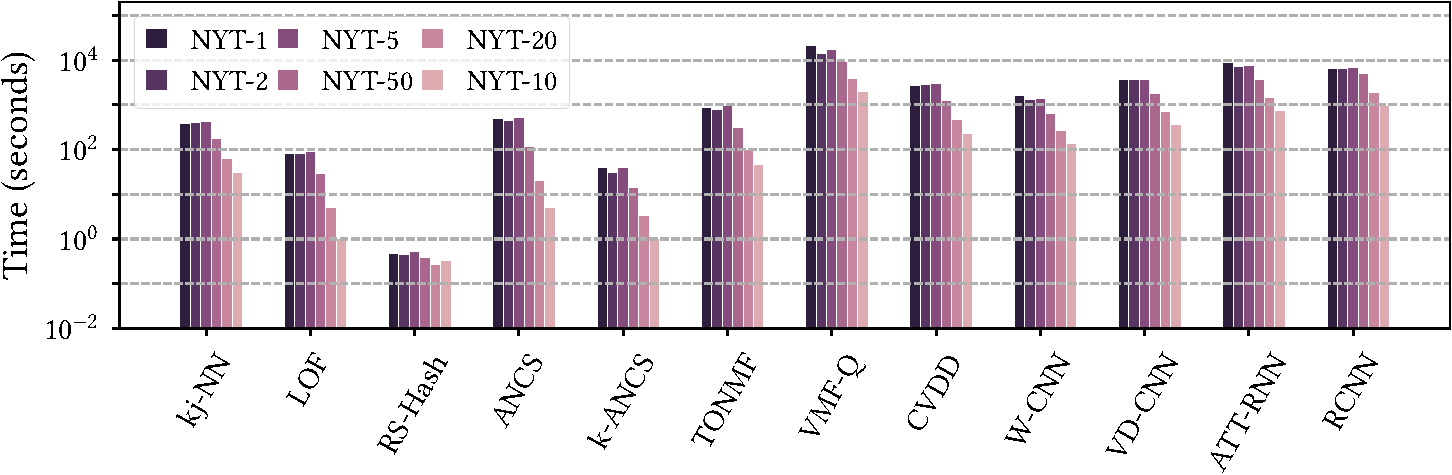
\includegraphics[width=\linewidth]{part4-figures/runtime-3-crop-compressed.pdf}
	\caption{Execution time of each approach.}
	\label{fig:runtime}
\end{figure} %EF: I think I am actually neglecting the step to compute representativeness (it is the most expensive... -> But could be done in a way that is more efficient)

\subsubsection{Execution Time}
Figure \ref{fig:runtime} graphs the execution time for each approach. We neglect the common preprocessing time for each of them and report the sum of training and testing time. \gls{RS-Hash} is extremely fast, but as we saw the performance is not better than guessing. \gls{LOF} and \gls{k-ANCS}, which leverage index support, are relatively fast. 
Our method, \gls{kj-NN}, is only slightly slower than \gls{LOF} but seems to scale better (observe the difference in execution time between NYT-1 and NYT-10). The other methods appear slower. 

\subsection{Interpretation}

The design of our method gives way to interpretable results. To find similar documents, we can simply perform a nearest-neighbour search in the embedding space. We find in turn the most representative phrases for a given outlier $\gls{d}_{\textit{out}}$ via a similar approach as in preprocessing (see Section~\ref{sec:kjNNframework}), 
with this time only two classes: an outlier class $\gls{c}_{\textit{out}}$ containing the $k$-neighbourhood of document $\gls{d}$, i.e., $\mathcal{K}(\gls{d}) \cup  \gls{d}$ and a class $\gls{c}_{\textit{in}}$ containing the rest of the documents in the corpus. 

Figure \ref{fig:examples} shows the two top-ranked Type~O and Type~M outliers we found in NYT-1, along with the most representative phrases and excerpts from the most similar documents. 

It is interesting to see that the three nearest neighbours of the Type~O outlier either relate to building construction projects or political decisions in education (or both). 
Actually, the ground truth label `\textit{Education}' even appears at position five within the most representative phrases --- a useful information in practice. 

With the Type~M outlier, the nearest documents all relate to science and business in some way, and the top phrases (energy, fuel, \dots) strongly relate to their specific topic. 

We then run our approach on the ARXIV benchmark with all the ten classes. Figure \ref{fig:examples_arxiv} shows the top-ranked outliers. The Type~O outliers are indeed abnormal: they are not paper abstracts, so one should remove them from the corpus. 
The Type~M outlier is from \cite{DBLP:journals/corr/abs-1107-3663}. The authors chose to publish this article in the category \textit{cs.AI} (Artificial Intelligence), but our approach suggests that it should be under \textit{cs.CL} (Computation and Language). Intuitively, this makes sense, given the general topic of the abstract and the most representative phrases. 

\begin{figure*}
	\includegraphics[width=\linewidth]{part4-figures/examples-Large-compressed.pdf}
	\caption{Interpretation of Type O/M outliers (NYT-1 benchmark).}
	\label{fig:examples}
\end{figure*} 
%EF: IDEA: Maybe highly words which are representative with some coloring scheme 

\begin{figure*}
	\includegraphics[width=\linewidth]{part4-figures/examples_ARXIV-Large-compressed.pdf}
	\caption{Interpretation of Type O/M outliers (ARXIV benchmark).}
	\label{fig:examples_arxiv}
\end{figure*}
% EF: IDEA: Show the distribution of outliers in the ranking 

\section{Discussion}

We have studied the detection of text outliers in document directories. This task is challenging because text outliers are manifold, domain-specific, and the task is unsupervised. 

We observe that such outliers fall into two types: out-of-distribution (Type~O) and misclassified (Type~M) documents. We are first to propose an approach that (i) detects text outliers from multiple folders and (ii) effectively distinguishes between both outlier types. Our algorithm, \gls{kj-NN}, leverages self-supervision signals mined from an initial but imperfect classification. Interestingly, our experiments show that detecting both outlier types simultaneously leads to better performance % for each type 
than with existing approaches, which only deal with one type. Our method also yields interpretable results, by finding adequate alternative names for folders and by describing the particular semantics of text outliers. 

This chapter only addressed text outlier detection in the static setting, while text can also be seen as a stream of information. An interesting future work would be to combine it with our other methods, such as \acrshort{MCDE} (Chapter \ref{chapter:MCDE}) and \acrshort{S-MAB} (Chapter \ref{chapter:S-MAB}), similarly as in Chapter \ref{chapter:subspacesearch}. Doing so would facilitate Data Mining in massive streams of textual information, such as news feeds or twitter data. Text outlier detection in such a setting is an interesting application of Knowledge Discovery in high-dimensional data streams. 

%Using our results may increase the quality of large text archives by much. %EF: Maybe also assist annotators / improve user experience
%EF: We could also say that it could be useful as a recommendation system.  